\begin{beginningnote}
    Si tenga presente che alcuni termini utilizzati nel documento riportano la lettera \textbf{G} in apice, allo scopo di evidenziare le parole che assumono uno specifico significato nell'ambito del progetto. Per comprenderle in maniera corretta, si rimanda il lettore al documento ``Glossario", che contiene un elenco completo di tutte le terminologie utilizzate con relative definizioni, allo scopo di costruire un linguaggio uniforme che possa migliorare la comunicazione tra i componenti interni al gruppo e gli stakeholders\textsuperscript{G} esterni.   %inserire corsivo per ogni termine del glossario?
\end{beginningnote}

%unire scopo delcoumento e il progetto in un unica sezione  (e.g. introduzione) con due sottosezioni?
%%%%%%%%%%%%%%%%%%%%%%%%%%%%%%%%%%%
% SCOPO DEL DOCUMENTO
%%%%%%%%%%%%%%%%%%%%%%%%%%%%%%%%%%%

\section{Introduzione}

\subsection{Scopo del documento}\label{sec:scopo_del_documento}
\par Questo documento definisce come le attività di controllo della qualità saranno gestite durante il ciclo di vita del prodotto software. Include dettagli sui processi e standard da seguire per assicurare che il prodotto finale rispetti i requisiti di qualità specificati. Questo piano è fondamentale per garantire che il software sviluppato sia di alta qualità e soddisfi le aspettative dei clienti e degli stakeholder. Al suo interno contiene le metriche per misurare il livello di qualità di progetto in fase di sviluppo, in modo da poter migliorare alcune procedure se giudicate non conformi alle aspettative. Si prevede che il documento abbia natura incrementale, perché le metriche potrebbero essere aggiornate o riadattate in corso di progetto, a seconda delle esigenze e delle richieste da parte del committente.
\par Nel corso di progetto, l'accertamento della qualità sarà documentato allegando al documento le misurazioni delle attività di verifica con le metriche descritte.

%%%%%%%%%%%%%%%%%%%%%%%%%%%%%%%%%%%
% IL PROGETTO
%%%%%%%%%%%%%%%%%%%%%%%%%%%%%%%%%%%
\subsection{Il progetto}\label{sec:il_progetto}
\par Il progetto nasce nell'ambito dei \textbf{sistemi gestionali di magazzino}, meglio noti con il termine inglese di \textit{Warehouse Management Systems} (WMS), con l'obiettivo di risolvere una serie di problematiche derivanti dalle soluzioni tradizionali tuttora presenti sul mercato.
\par Il focus principale sarà migliorare la user experience, tramite la realizzazione di un applicativo che proponga all'utente un'interazione con il magazzino in un ambiente di lavoro 3D: questa soluzione, rispetto ai tradizionali sistemi 2D, garantirebbe una maggiore comprensione degli spazi, proponendo una visualizzazione più intuitiva e familiare del magazzino all'utente che, di conseguenza, sarà in grado di prendere decisioni organizzative più informate ed efficienti, ottimizzando i processi di logistica.
\par Per raggiungere questo obiettivo, l'ambiente di lavoro non può essere una semplice visualizzazione del magazzino. L'utente dovrà infatti poter:
\begin{itemize}
    \item Navigare l'ambiente 3D;
    \item Progettare la scaffalatura e modificarla nel tempo;
    \item Inserire, spostare e rimuovere prodotti negli scaffali.
\end{itemize}
Il progetto deve concretizzarsi nella realizzazione di una web app fruibile agli impiegati d'ufficio ed incentrata sulla visualizzazione 3D del magazzino.
\par Per visionare il capitolato\textsuperscript{G} e la documentazione del gruppo, si veda la sezione \hyperref[sec:riferimenti_esterni]{Riferimenti Esterni} del documento.

\newpage

%%%%%%%%%%%%%%%%%%%%%%%%%%%%%%%%%%%
% QUALITA' DI PROCESSO
%%%%%%%%%%%%%%%%%%%%%%%%%%%%%%%%%%%
\section{Obiettivi metrici di qualità}\label{sec:obiettivi_metrici}
In questa sezione si presentano i valori accettabili e ideali delle metriche, insieme ad una breve descrizione delle stesse. Le metriche descritte nel documento saranno identificate univocamente tramite un codice standardizzato secondo quanto definito nelle \textit{Norme di Progetto}, reperibili nella sezione \hyperref[sec:riferimenti_esterni]{Riferimenti Esterni} del documento.

\subsection{Qualità di processo}\label{sec:qualita_di_processo}
Questa sezione è dedicata alle metriche atte a misurare la qualità dei processi nel corso del progetto didattico, qui descritti seguendo lo standard \textbf{ISO/IEC 12207}, reperibile nella sezione \hyperref[sec:riferimenti_esterni]{Riferimenti Esterni} del documento. 
\subsubsection{Processi primari}
\paragraph{Fornitura}
Uno dei compiti principali del processo di fornitura è la gestione delle procedure e delle risorse necessarie a garantire il raggiungimento degli obiettivi di progetto. Per questo motivo, le metriche di qualità adottate in questo processo hanno lo scopo di misurare come il progetto si sta muovendo rispetto alla sua pianificazione originaria, in termini di costi previsti in partenza rispetto ai costi effettivi nel corso di progetto.
\par Risulta subito evidente il fatto che delle semplici metriche di monitoraggio dei tempi non sono abbastanza per comprendere lo stato effettivo del progetto (molte ore di lavoro non significano sempre che il prodotto da realizzare è a buon punto) e per questo non possono garantire un buon livello di qualità. Per questo motivo, il gruppo ha scelto di utilizzare le metriche proposte dal metodo \textbf{Earned Value}, che si propone di misurare la quantità di lavoro effettivamente eseguito su un progetto.
\par Gli acronimi utilizzati nelle metriche faranno riferimento a quelli proposti dallo standard, reperibili al link sulle metriche di progetto nella sezione \hyperref[sec:riferimenti_esterni]{Riferimenti Esterni}. Per una lettura più immediata del documento si riportano i termini principali:
\begin{table}[h!]
\centering
\def\arraystretch{1.5}
\begin{tabular}{ |m{2cm}|m{4cm}|m{8cm}| }
\hline
\rowcolor{lightgray!30}
\textbf{Acronimo} & \textbf{Nome} & \textbf{Significato}\\
\hline
\textbf{PV} & Planned Value & Costo pianificato per realizzare le attività di progetto alla data corrente.\\
\hline
\textbf{AC} & Actual Cost & Costo effettivamente sostenuto alla data corrente.\\
\hline
\textbf{EV} & Earned Value & Valore delle attività realizzate alla data corrente.\\
\hline
\textbf{BAC} & Budget at Completion & Indica il valore iniziale previsto per la realizzazione del progetto.\\
\hline
\textbf{ETC} & Estimate to Complete & Valore stimato per la realizzazione delle rimanenti attività necessarie al completamento del progetto.\\
\hline
\textbf{EAC} & Estimated at Completion & Indica la revisione del BAC rispetto allo stato corrente del progetto (EAC = AC + ETC).\\
\hline
\textbf{CV} & Cost Variance & Calcola il valore del costo realmente maturato rispetto al costo effettivo (CV = EV - AC).\\
\hline
\textbf{SV} & Schedule Variance & Calcola le tempistiche effettive (se si è in anticipo o ritardo) rispetto alla schedulazione delle attività pianificate (SV = EV - PV).\\
\hline
\textbf{BV} & Budget Variance & Indica se alla data corrente si è speso di più o di meno rispetto a quanto previsto (BV = PV - AC).\\
\hline

\end{tabular}
\caption{Acronimi per le metriche del processo di Fornitura}
\end{table}

\newpage
Le metriche sono stabilite di conseguenza:
\begin{table}[h!]
\rowcolors{2}{lightgray!30}{white}
\centering
\def\arraystretch{1.5}
\begin{tabular}{ |>{\centering\arraybackslash}m{2.5cm}|>{\centering\arraybackslash}m{5.5cm}|>{\centering\arraybackslash}m{3cm}|>{\centering\arraybackslash}m{3cm}| }
\hline
\rowcolor{black}
\textbf{\color{white} Codice} & \textbf{\color{white} Descrizione} & \textbf{\color{white} Valore accettabile} & \textbf{\color{white} Valore ottimale}\\
\hline
MPC1-EAC & Si vuole che il costo attuale sia quanto più possibile in linea con quello pianificato originariamente & Errore massimo del $\pm 5$\% rispetto a BAC & = BAC \\
\hline
MPC2-CV & Si vuole che il valore delle attività completate (EV) sia corrispondente o maggiore del costo sostenuto (AC) & $\geq$ -10\% & $\geq$ 0 \\
\hline
MPC3-SV & Si vuole che il progetto produca con maggiore o uguale velocità rispetto a quanto pianificato & $\geq$ -10\% & $\geq$ 0 \\
\hline
MPC4-BV & Si vuole che i costi previsti nella pianificazione iniziale corrispondano a quelli effettivi & Errore massimo del $\pm 10$\% & 0 \\
\hline
MPC5-PV & I costi pianificati per le attività di progetto non devono sforare i costi originariamente pianificati & - & La somma dei costi di volta in volta deve essere $\leq$ BAC \\
\hline
MPC6-AC & I costi effettivi per le attività di progetto non devono sforare i costi pianificati nella revisione del BAC & - & La somma dei costi di volta in volta deve essere $\leq$ EAC \\
\hline
MPC7-EV & Il valore effettivo per le attività di progetto non deve sforare i costi pianificati nella revisione del BAC & - & La somma dei costi di volta in volta deve essere $\leq$ EAC \\
\hline
\end{tabular}
\caption{Metriche del processo di Fornitura}
\end{table}

\paragraph{Sviluppo}
Il processo di sviluppo definisce i compiti e le attività che il gruppo deve svolgere per la
realizzazione del prodotto software concorde con le esigenze del proponente ed, in particolare, si occupa delle attività di analisi dei requisiti, progettazione e codifica. Le metriche di qualità individuate per questo processo sono relative soprattutto alle ultime due attività.
\subparagraph{Progettazione.} Per assicurare qualità nella fase di progettazione si è ritenuto importante utilizzare le metriche di \textbf{Structural fan-in} e \textbf{fan-out}, applicate alle procedure con i seguenti acronimi:
\begin{table}[h!]
\centering
\def\arraystretch{1.5}
\begin{tabular}{ |m{2cm}|m{4cm}|m{8cm}| }
\hline
\rowcolor{lightgray!30}
\textbf{Acronimo} & \textbf{Nome} & \textbf{Significato}\\
\hline
\textbf{SFINp} & Structural fan-in (procedure) & Numero di procedure che chiamano una specifica procedura.\\
\hline
\textbf{SFOUTp} & Structural fan-out (procedure) & Numero di procedure che una specifica procedura chiama.\\
\hline
\end{tabular}
\caption{Acronimi per le metriche del processo di Sviluppo (Progettazione)}
\end{table}

\newpage
Le regole da applicare alle metriche sono dunque le seguenti:
\begin{table}[h!]
\rowcolors{2}{lightgray!30}{white}
\centering
\def\arraystretch{1.5}
\begin{tabular}{ |>{\centering\arraybackslash}m{4cm}|>{\centering\arraybackslash}m{5.5cm}|>{\centering\arraybackslash}m{5cm}| }
\hline
\rowcolor{black}
\textbf{\color{white} Codice} & \textbf{\color{white} Descrizione} & \textbf{\color{white} Valore desiderabile}\\
\hline
MPC8-SFINp & Si vuole che le procedure progettate vengano riutilizzate & Alto (riutilizzo di codice) \\
\hline
MPC9-SFOUTp & Si vuole che le procedure non siano fortemente accoppiate fra loro & Basso (bassa dipendenza tra procedure) \\
\hline
\end{tabular}
\caption{Metriche del processo di Sviluppo (Progettazione)}
\end{table}


\subparagraph{Codifica.}
Con l'attività di codifica, i programmatori si impegnano a concretizzare quanto prodotto con l'attività di progettazione attraverso la programmazione del software vero e proprio.
Lo scopo è quello di ottenere un prodotto software che rispetti i requisti e le richieste concordati con il proponente e che ne garantisca la qualità. Per raggiungere questi obiettivi si utilizzano metriche che cercano di limitare gli errori introdotti nel codice, in particolare:
\begin{table}[h!]
\centering
\def\arraystretch{1.5}
\begin{tabular}{ |m{2cm}|m{2.5cm}|m{9.5cm}| }
\hline
\rowcolor{lightgray!30}
\textbf{Acronimo} & \textbf{Nome} & \textbf{Significato}\\
\hline
\textbf{CCH} & Code churn & Indica il numero di modifiche, aggiunte e cancellazioni apportate nel tempo ad una certa area di codice, in particolare nell'ambito di progetto, si intende modifiche apportate ad una procedura. Più sono le modifiche, più aumenta il rischio di introdurre errori nel codice. Un alto valore di nuove linee di codice potrebbe anche indicare basso riutilizzo di codice.\\
\hline
\textbf{NB} & Number of bugs & Indica il numero di bug ed errori presenti nel software.\\
\hline
\textbf{CC} & Cyclomatic complexity & Misura la complessità del codice calcolando il numero di percorsi indipendenti (contando cioè il numero di ``decisioni prese" nel codice sorgente). Un alto valore di complessità ciclomatica\textsuperscript{G} indica codice difficile da comprendere, mantenere e testare.\\
\hline
\end{tabular}
\caption{Acronimi per le metriche del processo di Sviluppo (Codifica)}
\end{table}
\par Le regole di qualità sono applicate alle metriche nel seguente modo:
\begin{table}[h!]
\rowcolors{2}{lightgray!30}{white}
\centering
\def\arraystretch{1.5}
\begin{tabular}{ |>{\centering\arraybackslash}m{2.5cm}|>{\centering\arraybackslash}m{5.5cm}|>{\centering\arraybackslash}m{3cm}|>{\centering\arraybackslash}m{3cm}| }
\hline
\rowcolor{black}
\textbf{\color{white} Codice} & \textbf{\color{white} Descrizione} & \textbf{\color{white} Valore accettabile} & \textbf{\color{white} Valore ottimale}\\
\hline
MPC10-CCH & Il numero di modifiche apportate alla singola procedura deve essere quanto più basso possibile & Massimo 20\% di modifiche sul codice totale della procedura & 0 \\
\hline
MPC11-NB & Si vuole che il numero di bug ed errori nel codice sia quanto più basso possibile & $\leq$ 5 & 0 \\
\hline
MPC12-CC & Il codice deve essere mantenuto semplice, facilitando comprensione, manutenzione e test & $\leq$ 15 & $\leq$ 10 \\
\hline
\end{tabular}
\caption{Metriche del processo di Sviluppo (Codifica)}
\end{table}

\subsubsection{Processi di supporto}
\paragraph{Documentazione}
La documentazione prodotta nel corso del progetto deve essere un valido supporto al gruppo e agli stakeholders per comprendere meglio il codice prodotto, le decisioni prese e la gestione organizzativa. Per questo motivo, le metriche di qualità sulla documentazione si concentrano sulla leggibilità e sul controllo degli errori ortografici. Le metriche in questione sono le seguenti:
\begin{table}[h!]
\centering
\def\arraystretch{1.5}
\begin{tabular}{ |m{2cm}|m{4.5cm}|m{7.5cm}| }
\hline
\rowcolor{lightgray!30}
\textbf{Acronimo} & \textbf{Nome} & \textbf{Significato}\\
\hline
\textbf{EOD} & Errori ortografici per documento & Indica il numero di errori ortografici individuati per documento.\\
\hline
\textbf{IG} & Indice Gulpease & Calcola la leggibilità di un testo in lingua italiana prendendo in considerazione la lunghezza della parola e la lunghezza della frase rispetto al numero di lettere. 
\begin{center}
    $89 + \ddfrac{300 * (num.\: frasi) - 10 * (num.\: lettere)}{(num.\: parole)} $
\end{center}\\
\hline
\end{tabular}
\caption{Acronimi per le metriche del processo di Documentazione}
\end{table}
\par Le regole di qualità sono applicate alle metriche nel seguente modo:
\begin{table}[h!]
\rowcolors{2}{lightgray!30}{white}
\centering
\def\arraystretch{1.5}
\begin{tabular}{ |>{\centering\arraybackslash}m{2.5cm}|>{\centering\arraybackslash}m{5.5cm}|>{\centering\arraybackslash}m{3cm}|>{\centering\arraybackslash}m{3cm}| }
\hline
\rowcolor{black}
\textbf{\color{white} Codice} & \textbf{\color{white} Descrizione} & \textbf{\color{white} Valore accettabile} & \textbf{\color{white} Valore ottimale}\\
\hline
MPC13-EOD & Si vogliono meno errori ortografici possibili per ciascun documento & $\leq 5$ & 0 \\
\hline
MPC14-IG & La documentazione deve essere di facile lettura & 30-100 & 40-100 \\
\hline
\end{tabular}
\caption{Metriche del processo di Documentazione}
\end{table}

\paragraph{Accertamento della qualità}
Lo scopo dell'accertamento della qualità è garantire che i processi e il prodotto siano conformi alle attese e soddisfino al meglio le richieste del proponente. A tal fine e per avere una valutazione oggettiva e quantificabile della qualità, si fa riferimento al presente \textit{Piano di Qualifica}, che riporta le metriche di qualità adottate dal gruppo nell'ambito del progetto.
\par Diventa quindi essenziale il soddisfacimento delle metriche preposte:
\begin{table}[h!]
\centering
\def\arraystretch{1.5}
\begin{tabular}{ |m{2cm}|m{3.5cm}|m{8.5cm}| }
\hline
\rowcolor{lightgray!30}
\textbf{Acronimo} & \textbf{Nome} & \textbf{Significato}\\
\hline
\textbf{MS} & Metriche soddisfatte & Indica la percentuale di metriche di qualità soddisfatte rispetto al totale delle metriche preposte.\\
\hline
\end{tabular}
\caption{Acronimi per le metriche del processo di Accertamento della qualità}
\end{table}
\par Con le seguenti regole:
\begin{table}[h!]
\rowcolors{2}{lightgray!30}{white}
\centering
\def\arraystretch{1.5}
\begin{tabular}{ |>{\centering\arraybackslash}m{2.5cm}|>{\centering\arraybackslash}m{5.5cm}|>{\centering\arraybackslash}m{3cm}|>{\centering\arraybackslash}m{3cm}| }
\hline
\rowcolor{black}
\textbf{\color{white} Codice} & \textbf{\color{white} Descrizione} & \textbf{\color{white} Valore accettabile} & \textbf{\color{white} Valore ottimale}\\
\hline
MPC15-MS & Il numero di metriche di qualità soddisfatte deve essere molto alto & 90\% & 100\% \\
\hline
\end{tabular}
\caption{Metriche del processo di Accertamento della qualità}
\end{table}

\newpage
\paragraph{Verifica}
Il processo di verifica ha lo scopo di determinare se i prodotti dei processi durante il corso del progetto rispettano i requisiti preposti. In particolare, si vuole enfatizzare la correttezza del codice prodotto attraverso le seguenti metriche:
\begin{table}[h!]
\centering
\def\arraystretch{1.5}
\begin{tabular}{ |m{2cm}|m{3.5cm}|m{8.5cm}| }
\hline
\rowcolor{lightgray!30}
\textbf{Acronimo} & \textbf{Nome} & \textbf{Significato}\\
\hline
\textbf{CCV} & Code coverage & Misura la quantità di codice (in percentuale) coperta dai test rispetto al totale del codice sorgente.\\
\hline
\textbf{TP} & Test passati & Misura la quantità di test (in percentuale) eseguiti con successo.\\
\hline
\end{tabular}
\caption{Acronimi per le metriche del processo di Verifica}
\end{table}
\par Con le seguenti regole:
\begin{table}[h!]
\rowcolors{2}{lightgray!30}{white}
\centering
\def\arraystretch{1.5}
\begin{tabular}{ |>{\centering\arraybackslash}m{2.5cm}|>{\centering\arraybackslash}m{5.5cm}|>{\centering\arraybackslash}m{3cm}|>{\centering\arraybackslash}m{3cm}| }
\hline
\rowcolor{black}
\textbf{\color{white} Codice} & \textbf{\color{white} Descrizione} & \textbf{\color{white} Valore accettabile} & \textbf{\color{white} Valore ottimale}\\
\hline
MPC16-CCV & Si vuole che la percentuale di codice coperta da test sia molto alta & $\geq$ 90\% & 100\% \\
\hline
MPC17-TP & Si vuole che tutti i test siano eseguiti con successo & 100\% & 100\% \\
\hline
\end{tabular}
\caption{Metriche del processo di Verifica}
\end{table}
\newpage

\subsection{Qualità di prodotto}
L'obiettivo delle metriche definite in questa sezione è controllare la qualità del prodotto realizzato nel corso del progetto. Per questa ragione, diventa importante assicurarsi che il prodotto sia conforme alle richieste del proponente e che possieda le caratteristiche proprie di un software di qualità.
\subsubsection{Customer needs}
Si definiscono le seguenti metriche:
\begin{table}[h!]
\centering
\def\arraystretch{1.5}
\begin{tabular}{ |m{2cm}|m{5.5cm}|m{6.5cm}| }
\hline
\rowcolor{lightgray!30}
\textbf{Acronimo} & \textbf{Nome} & \textbf{Significato}\\
\hline
\textbf{ROB} & Copertura dei requisiti obbligatori & Indica il valore (in percentuale) di requisiti obbligatori che il prodotto soddisfa.\\
\hline
\textbf{RDE} & Copertura dei requisiti desiderabili & Indica il valore (in percentuale) di requisiti desiderabili che il prodotto soddisfa.\\
\hline
\end{tabular}
\caption{Acronimi per le metriche riguardanti i Customer needs}
\end{table}
\par Con le seguenti regole:
\begin{table}[h!]
\rowcolors{2}{lightgray!30}{white}
\centering
\def\arraystretch{1.5}
\begin{tabular}{ |>{\centering\arraybackslash}m{2.5cm}|>{\centering\arraybackslash}m{5.5cm}|>{\centering\arraybackslash}m{3cm}|>{\centering\arraybackslash}m{3cm}| }
\hline
\rowcolor{black}
\textbf{\color{white} Codice} & \textbf{\color{white} Descrizione} & \textbf{\color{white} Valore accettabile} & \textbf{\color{white} Valore ottimale}\\
\hline
MPD1-ROB & I requisiti obbligatori devono essere tutti soddisfatti & 100\% & 100\% \\
\hline
MPD2-RDE & I requisiti desiderabili devono essere soddisfatti in buona parte & 70\% & 100\% \\
\hline
\end{tabular}
\caption{Metriche riguardanti i Customer needs}
\end{table}

\subsubsection{Efficienza}
Si definiscono le seguenti metriche:
\begin{table}[h!]
\centering
\def\arraystretch{1.5}
\begin{tabular}{ |m{2cm}|m{5.5cm}|m{6.5cm}| }
\hline
\rowcolor{lightgray!30}
\textbf{Acronimo} & \textbf{Nome} & \textbf{Significato}\\
\hline
\textbf{ART} & Average response time & Misura il tempo medio che il prodotto software impiega per rispondere agli input forniti dall'utente.\\
\hline
\end{tabular}
\caption{Acronimi per le metriche riguardanti l'Efficienza}
\end{table}
\par Con le seguenti regole:
\begin{table}[h!]
\rowcolors{2}{lightgray!30}{white}
\centering
\def\arraystretch{1.5}
\begin{tabular}{ |>{\centering\arraybackslash}m{2.5cm}|>{\centering\arraybackslash}m{5.5cm}|>{\centering\arraybackslash}m{3cm}|>{\centering\arraybackslash}m{3cm}| }
\hline
\rowcolor{black}
\textbf{\color{white} Codice} & \textbf{\color{white} Descrizione} & \textbf{\color{white} Valore accettabile} & \textbf{\color{white} Valore ottimale}\\
\hline
MPD3-ART & Il prodotto deve essere veloce nel tempo di risposta & $<$ 3 sec. & $\leq$ 1 sec. \\
\hline
\end{tabular}
\caption{Metriche riguardanti l'Efficienza}
\end{table}

\subsubsection{Usabilità}
\par Si definiscono le seguenti metriche:
\begin{table}[h!]
\centering
\def\arraystretch{1.5}
\begin{tabular}{ |m{2cm}|m{5.5cm}|m{6.5cm}| }
\hline
\rowcolor{lightgray!30}
\textbf{Acronimo} & \textbf{Nome} & \textbf{Significato}\\
\hline
\textbf{PC} & Profondità di click per operazione & Misura il numero di click che l'utente deve fare per raggiungere un determinato obiettivo. Un numero troppo alto provoca frustrazione e difficoltà di utilizzo.\\
\hline
\textbf{CFO} & Comprensibilità funzioni offerte & Misura la quantità (in percentuale) di funzioni offerte che l'utente riesce ad individuare ed utilizzare con facilità.\\
\hline
\end{tabular}
\caption{Acronimi per le metriche riguardanti l'Usabilità}
\end{table}
\newpage
\par Con le seguenti regole:
\begin{table}[h!]
\rowcolors{2}{lightgray!30}{white}
\centering
\def\arraystretch{1.5}
\begin{tabular}{ |>{\centering\arraybackslash}m{2.5cm}|>{\centering\arraybackslash}m{5.5cm}|>{\centering\arraybackslash}m{3cm}|>{\centering\arraybackslash}m{3cm}| }
\hline
\rowcolor{black}
\textbf{\color{white} Codice} & \textbf{\color{white} Descrizione} & \textbf{\color{white} Valore accettabile} & \textbf{\color{white} Valore ottimale}\\
\hline
MPD4-PC & L'utente deve essere facilitato nell'interazione con il prodotto software & $\leq$ 7 & $\leq$ 5 \\
\hline
MPD5-CFO & L'utente deve comprendere facilmente quali sono e come si comportano le funzioni offerte & $\geq$ 90\% & 100\% \\
\hline
\end{tabular}
\caption{Metriche riguardanti l'Usabilità}
\end{table}

\subsubsection{Portabilità su altre piattaforme}
Su richiesta del committente, il software prodotto deve essere una Web Application. Come tale, risulta essenziale assicurarsi che il prodotto sia utilizzabile tramite tutti i browser maggiormente utilizzati nel mercato.
\par Le applicazioni che sono state considerate sono:
\begin{itemize}
    \item Google Chrome,
    \item Mozilla Firefox,
    \item Microsoft Edge,
    \item Safari,
    \item Opera.
\end{itemize}
Si definiscono dunque le seguenti metriche:
\begin{table}[h!]
\centering
\def\arraystretch{1.5}
\begin{tabular}{ |m{2cm}|m{5.5cm}|m{6.5cm}| }
\hline
\rowcolor{lightgray!30}
\textbf{Acronimo} & \textbf{Nome} & \textbf{Significato}\\
\hline
\textbf{PPT} & Portabilità su piattaforme & Indica la percentuale di piattaforme (tra quelle prese in considerazione) su cui il prodotto software è utilizzabile.\\
\hline
\end{tabular}
\caption{Acronimi per le metriche riguardanti la Portabilità su piattaforme}
\end{table}
\par Con le seguenti regole:
\begin{table}[h!]
\rowcolors{2}{lightgray!30}{white}
\centering
\def\arraystretch{1.5}
\begin{tabular}{ |>{\centering\arraybackslash}m{2.5cm}|>{\centering\arraybackslash}m{5.5cm}|>{\centering\arraybackslash}m{3cm}|>{\centering\arraybackslash}m{3cm}| }
\hline
\rowcolor{black}
\textbf{\color{white} Codice} & \textbf{\color{white} Descrizione} & \textbf{\color{white} Valore accettabile} & \textbf{\color{white} Valore ottimale}\\
\hline
MPD6-PPT & Il prodotto deve essere utilizzabile su tutti i browser principali. & 100\% & 100\% \\
\hline
\end{tabular}
\caption{Metriche riguardanti la Portabilità su piattaforme}
\end{table}

\newpage
\section{Specifica dei test}\label{sec:test}
\par Questa sezione è dedicata alla descrizione dei vari tipi di test che verranno effettuati per assicurare la qualità e l'affidabilità del software.
I test utili all’interno di un progetto sono:
\begin{itemize}
    \item \textbf{Test di unità};
    \item \textbf{Test di integrazione};
    \item \textbf{Test di sistema};
    %\item \textbf{Test di regressione};
    \item \textbf{Test di accettazione}.
\end{itemize}
I test descritti nel documento saranno identificati univocamente tramite un codice standardizzato secondo quanto definito nelle \textit{Norme di Progetto}. Inoltre, si noti che nella descrizione dei test saranno presenti riferimenti a classi, procedure e componenti meglio descritti nel documento di \textit{Specifica Tecnica}.
Tali documenti sono reperibili nella sezione \hyperref[sec:riferimenti_esterni]{Riferimenti Esterni} del documento.
\\ 
I test verranno elencati riportando lo stato, che può essere:
\begin{itemize}
    \item \textbf{NI}: se il test non è stato ancora implementato;
    \item \textbf{S}: se il test è stato implementato ed ha avuto esito positivo, i.e. test superato;
    \item \textbf{NS}: se il test è stato implementato ed ha avuto esito negativo, i.e. test non superato.    
\end{itemize}

\subsection{Test di Unità}
\par I test di unità sono di basso livello e mirano a testare le singole unità dell'applicativo software in isolamento. Il concetto di unità si fa corrispondere generalmente alle funzioni per la programmazione procedurale, oppure a metodi e classi per la programmazione ad oggetti.
\par Sono i più economici da implementare, possono essere scritti più velocemente rispetto agli altri e generalmente vengono eseguiti in maniera automatica (rendendo veloce anche la loro esecuzione e ripetizione). Inoltre, permettono di individuare un problema in maniera più immediata, evitando che si propaghi nel software.
\vspace{0.5cm} \\ Le tabelle che seguono mostrano il registro dei test effettuati, organizzati per come si prevede di suddividere la realizzazione dell'applicativo (e cioè per feature\textsuperscript{G}), con una breve valutazione e retrospettiva per ciascuna feature.

\subsubsection{Feature model}
\renewcommand{\arraystretch}{1.5}
\rowcolors{2}{gray!10!}{white}
\begin{xltabular}{0.9\textwidth}{X | p{0.6\textwidth} | p{0.1\textwidth} }
    \rowcolor{black}
    \textbf{\color{white} Test} & \textbf{\color{white} Descrizione} & \textbf{\color{white} Stato}\\ 
    \hline
    \endhead
    \caption{Tabella dei test di unità per feature/model} 
    \label{tab:test_sistema}
    \endlastfoot
    %%%%%%%%%%%% Product
    TU-1 & Product deve essere implementato correttamente & S\\
    TU-1.1 & Product deve ritornare il nome corretto & S\\
    TU-1.2 & Product deve ritornare il colore corretto & S\\
    TU-1.3 & Product deve ritornare l'id corretto & S\\
    TU-1.4 & Product deve impostare un nuovo nome in maniera corretta & S\\
    TU-1.5 & Product deve impostare un nuovo colore in maniera corretta & S\\

    %%%%%%%%%%%% Bin
    TU-2 & Bin\textsuperscript{G} deve essere implementato correttamente & S\\
    TU-2.1 & Bin deve avere il productId di default uguale a null & S\\
    TU-2.2 & Bin deve avere lo stato di default uguale a EMPTY & S\\
    TU-2.3 & Bin deve ritornare l'id corretto & S\\
    TU-2.4 & Bin deve ritornare il productId corretto & S\\
    TU-2.5 & Bin deve ritornare lo stato corretto & S\\
    TU-2.6 & Bin deve impostare un nuovo productId in maniera corretta & S\\
    TU-2.7 & Bin deve impostare un nuovo stato in maniera corretta & S\\
    TU-2.8 & binState deve avere la proprietà EMPTY & S\\
    TU-2.9 & binState deve avere la proprietà OUTGOING & S\\
    TU-2.10 & binState deve avere la proprietà INCOMING & S\\
    TU-2.11 & binState deve avere la proprietà STILL & S\\
    
    %%%%%%%%%%%% Shelf
    TU-3 & Shelf deve essere implementato correttamente & S\\
    TU-3.1 & Shelf deve ritornare il nome corretto & S\\
    TU-3.2 & Shelf deve ritornare la binSize corretta & S\\
    TU-3.3 & Shelf deve ritornare la larghezza corretta & S\\
    TU-3.4 & Shelf deve ritornare l'altezza corretta & S\\
    TU-3.5 & Shelf deve ritornare la posizione corretta & S\\
    TU-3.6 & Shelf deve ritornare isFlipped corretto & S\\
    TU-3.7 & Shelf deve ritornare l'id corretto & S\\
    TU-3.8 & Shelf deve impostare un nuovo nome in maniera corretta & S\\
    TU-3.9 & Shelf deve impostare una nuova binSize in maniera corretta & S\\
    TU-3.10 & Shelf deve impostare una nuova altezza in maniera corretta & S\\
    TU-3.11 & Shelf deve impostare una nuova larghezza in maniera corretta & S\\
    TU-3.12 & Shelf deve impostare una nuova posizione in maniera corretta & S\\
    TU-3.13 & Shelf deve impostare un nuovo isFlipped in maniera corretta & S\\
    TU-3.14 & I bin di Shelf devono essere di tipo Bin & S\\
    TU-3.15 & I bin di Shelf devono avere un numero di colonne pari alla larghezza di Shelf & S\\
    TU-3.16 & I bin di Shelf devono avere un numero di righe pari all'altezza di Shelf & S\\
    TU-3.17 & I bin di Shelf devono avere id unici & S\\
    TU-3.18 & I bin di Shelf devono aumentare all'aumentare della larghezza di Shelf & S\\
    TU-3.19 & I bin di Shelf devono aumentare all'aumentare dell'altezza di Shelf & S\\
    TU-3.20 & I bin di Shelf devono diminuire alla diminuzione della larghezza di Shelf & S\\
    TU-3.21 & I bin di Shelf devono diminuire alla diminuzione della lunghezza di Shelf & S\\
    TU-3.22 & La larghezza di Shelf non deve diminuire se i bin coinvolti sono non-vuoti & S\\
    TU-3.23 & L'altezza di Shelf non deve diminuire se i bin coinvolti sono non-vuoti & S\\
    TU-3.24 & I bin di Shelf possono essere impostati solo da scaffalature della stessa dimensione & S\\
    TU-3.25 & I bin di Shelf devono avere l'id che corrisponde a shelf.id+i+j dove i e j sono indici della matrice & S\\
    TU-3.26 & I bin di una Shelf con id personalizzato devono avere l'id che corrisponde a shelf.id+i+j dove i e j sono indici della matrice & S\\
    TU-3.27 & I bin di Shelf devono essere impostati in maniera corretta & S\\
    TU-3.28 & ShelfError deve ritornare il messaggio corretto & S\\

    %%%%%%%%%%%% Movement
    TU-4 & Movement deve essere implementato correttamente & S\\
    TU-4.1 & Movement deve ritornare il corretto fromId & S\\
    TU-4.2 & Movement deve ritornare il corretto fromRow & S\\
    TU-4.3 & Movement deve ritornare il corretto fromCol & S\\
    TU-4.4 & Movement deve ritornare il corretto toId & S\\
    TU-4.5 & Movement deve ritornare il corretto toRow & S\\
    TU-4.6 & Movement deve ritornare il corretto toCol & S\\
    TU-4.7 & Movement deve ritornare il corretto id & S\\
    TU-4.8 & Movement deve impostare un nuovo fromId in maniera corretta & S\\
    TU-4.9 & Movement deve impostare un nuovo fromRow in maniera corretta & S\\
    TU-4.10 & Movement deve impostare un nuovo fromCol in maniera corretta & S\\
    TU-4.11 & Movement deve impostare un nuovo toId in maniera corretta & S\\
    TU-4.12 & Movement deve impostare un nuovo toRow in maniera corretta & S\\
    TU-4.13 & Movement deve impostare un nuovo toCol in maniera corretta & S\\

    %%%%%%%%%%%% whsSlice
    TU-5 & whsSlice deve essere implementato correttamente & S\\
    TU-5.1 & whsSlice deve impostare un nuovo nome del magazzino in maniera corretta & S\\
    TU-5.2 & whsSlice non deve impostare il nome del magazzino se la lunghezza è $>$ 20, deve invece impostare un errore & S\\
    TU-5.3 & whsSlice non deve impostare il nome del magazzino se i caratteri sono diversi da lettere, numeri e underscore, deve invece impostare un errore & S\\
    TU-5.4 & whsSlice non deve impostare il nome del magazzino se il nome è vuoto, deve invece impostare un errore & S\\
    TU-5.5 & whsSlice deve impostare il poligono del magazzino in maniera corretta & S\\
    TU-5.6 & whsSlice non deve impostare il poligono del magazzino se la lunghezza dei punti è $<$ 3, deve invece impostare un errore & S\\
    TU-5.7 & whsSlice non deve impostare il poligono del magazzino se la profondità è $>$ 1000, deve invece impostare un errore & S\\
    TU-5.8 & whsSlice non deve impostare il poligono del magazzino se la larghezza è $>$ 1000, deve invece impostare un errore & S\\
    TU-5.9 & whsSlice non deve impostare il poligono del magazzino se l'altezza è $>$ 50, deve invece impostare un errore & S\\
    TU-5.10 & whsSlice non deve impostare il poligono del magazzino se la larghezza è $<$ 0.01, deve invece impostare un errore & S\\
    TU-5.11 & whsSlice non deve impostare il poligono del magazzino se la profondità è $<$ 0.01, deve invece impostare un errore & S\\
    TU-5.12 & whsSlice non deve impostare il poligono del magazzino se l'altezza è $<$ 0.01, deve invece impostare un errore & S\\
    TU-5.13 & whsSlice deve impostare la base rettangolare del magazzino in maniera corretta & S\\
    TU-5.14 & whsSlice non deve impostare la base rettangolare del magazzino se la larghezza è vuota, deve invece impostare un errore & S\\
    TU-5.15 & whsSlice non deve impostare la base rettangolare del magazzino se la profondità è vuota, deve invece impostare un errore & S\\
    TU-5.16 & whsSlice non deve impostare la base rettangolare del magazzino se l'altezza è vuota, deve invece impostare un errore & S\\
    TU-5.17 & whsSlice non deve impostare la base rettangolare del magazzino se la larghezza è $>$ 1000, deve invece impostare un errore & S\\
    TU-5.18 & whsSlice non deve impostare la base rettangolare del magazzino se la profondità è $>$ 1000, deve invece impostare un errore & S\\
    TU-5.19 & whsSlice non deve impostare la base rettangolare del magazzino se l'altezza è $>$ 50, deve invece impostare un errore & S\\
    TU-5.20 & whsSlice non deve impostare la base rettangolare del magazzino se la larghezza è $<$ 0.01, deve invece impostare un errore & S\\
    TU-5.21 & whsSlice non deve impostare la base rettangolare del magazzino se la profondità è $<$ 0.01, deve invece impostare un errore & S\\
    TU-5.22 & whsSlice non deve impostare la base rettangolare del magazzino se l'altezza è $<$ 0.01, deve invece impostare un errore & S\\
    
    %%%%%%%%%%%% productsSlice
    TU-6 & productsSlice deve essere implementato correttamente & S\\
    TU-6.1 & productsSlice deve impostare l'elenco dei prodotti in maniera corretta & S\\
    TU-6.2 & productsSlice non deve impostare l'elenco dei prodotti se ci sono nomi duplicati, deve invece impostare un errore & S\\
    TU-6.3 & productsSlice non deve impostare l'elenco dei prodotti se ci sono id duplicati, deve invece impostare un errore & S\\
    TU-6.4 & productsSlice deve aggiungere un nuovo prodotto in maniera corretta & S\\
    TU-6.5 & productsSlice non deve aggiungere un nuovo prodotto se il nome esiste già, deve invece impostare un errore & S\\
    TU-6.6 & productsSlice deve rimuovere un prodotto in maniera corretta & S\\
    TU-6.7 & productsSlice deve aggiornare il nome di un prodotto in maniera corretta & S\\
    TU-6.8 & productsSlice non deve aggiornare il nome di un prodotto se esiste già,
    deve invece impostare un errore & S\\
    TU-6.9 & productsSlice deve aggiornare il colore di un prodotto in maniera corretta & S\\
    TU-6.10 & productsSlice deve svuotare le scaffalature quando rimuove un prodotto & S\\

    %%%%%%%%%%%% shelvesSlice
    TU-7 & shelvesSlice deve essere implementato correttamente & S\\
    TU-7.1 & shelvesSlice deve impostare l'elenco delle scaffalature in maniera corretta & S\\
    TU-7.2 & shelvesSlice non deve impostare l'elenco delle scaffalature se ci sono nomi duplicati, deve invece impostare un errore & S\\
    TU-7.3 & shelvesSlice non deve impostare l'elenco delle scaffalature se ci sono id duplicati, deve invece impostare un errore & S\\
    TU-7.4 & shelvesSlice deve aggiungere una nuova scaffalatura in maniera corretta & S\\
    TU-7.5 & shelvesSlice non deve aggiungere una nuova scaffalatura se l'altezza è maggiore dell'altezza del magazzino, deve invece impostare un errore & S\\
    TU-7.6 & shelvesSlice non deve aggiungere una nuova scaffalatura se il nome esiste già, deve invece impostare un errore & S\\
    TU-7.7 & shelvesSlice deve inserire un prodotto in maniera corretta in un bin vuoto & S\\
    TU-7.8 & shelvesSlice deve impostare lo stato a STILL quando inserisce un prodotto in un bin vuoto & S\\
    TU-7.9 & shelvesSlice non deve inserire un prodotto in un bin non-vuoto & S\\
    TU-7.10 & shelvesSlice deve rimuovere una scaffalatura in maniera corretta & S\\
    TU-7.11 & shelvesSlice deve rimuovere una scaffalatura solo se ha tutti i  bin vuoti & S\\
    TU-7.12 & shelvesSlice deve aggiornare il nome della scaffalatura in maniera corretta & S\\
    TU-7.13 & shelvesSlice non deve aggiornare il nome della scaffalatura se esiste già, deve invece impostare un errore & S\\
    TU-7.14 & shelvesSlice deve aggiornare la binSize della scaffalatura sin maniera corretta& S\\
    TU-7.15 & shelvesSlice deve aggiornare la larghezza della scaffalatura in maniera corretta & S\\
    TU-7.16 & shelvesSlice deve aggiornare l'altezza della scaffalatura in maniera corretta & S\\
    TU-7.17 & shelvesSlice non deve aggiornare l'altezza della scaffalatura se è maggiore dell'altezza del magazzino, deve invece impostare un errore & S\\
    TU-7.18 & shelvesSlice deve impostare un errore nella riduzione dell'altezza della scaffalatura se i bin sono non vuoti & S\\
    TU-7.19 & shelvesSlice deve impostare un errore nella riduzione della larghezza della scaffalatura se i bin sono non vuoti & S\\
    TU-7.20 & shelvesSlice deve aggiornare la posizione della scaffalatura in maniera corretta & S\\
    TU-7.21 & shelvesSlice non deve aggiornare la posizione della scaffalatura se fuori dal magazzino, deve invece impostare un errore & S\\
    TU-7.22 & shelvesSlice non deve aggiornare la posizione della scaffalatura se c'è un'intersezione, deve invece impostare un errore & S\\
    TU-7.23 & shelvesSlice deve aggiornare isFlipped della scaffalatura in maniera corretta & S\\
    TU-7.24 & shelvesSlice deve aggiornare lo stato del bin in maniera corretta & S\\
    TU-7.25 & shelvesSlice deve rimuovere un prodotto in maniera corretta & S\\
    TU-7.26 & shelvesSlice deve svuotare il bin quando rimuove un prodotto & S\\
    TU-7.27 & shelvesSlice deve poter ritornare i bin contenenti uno specifico prodotto & S\\  
    
    %%%%%%%%%%%% interactionsSlice
    TU-8 & interactionsSlice deve essere implementato correttamente & S\\
    TU-8.1 & interactionsSlice deve impostare gli id degli oggetti che si intersecano in maniera corretta & S\\
    TU-8.2 & interactionsSlice deve impostare la scaffalatura in movimentazione in maniera corretta & S\\
    TU-8.3 & interactionsSlice deve impostare la scaffalatura selezionata in maniera corretta & S\\
    TU-8.4 & La selezione di una scaffalatura deve deselezionare il bin & S\\
    TU-8.5 & La selezione di una scaffalatura deve deselezionare il prodotto & S\\
    TU-8.6 & interactionsSlice deve impostare il prodotto selezionato in maniera corretta & S\\
    TU-8.7 & La selezione di un prodotto deve deselezionare il bin & S\\
    TU-8.8 & La selezione di un prodotto deve deselezionare la scaffalatura & S\\
    TU-8.9 & interactionsSlice deve impostare il bin selezionato in maniera corretta & S\\
    TU-8.10 & La selezione di un bin deve deselezionare il prodotto & S\\
    TU-8.11 & La selezione di un bin deve deselezionare la scaffalatura & S\\
    TU-8.12 & interactionsSlice deve impostare le movimentazioni in maniera corretta & S\\
    TU-8.13 & interactionsSlice deve ordinare una movimentazione in maniera corretta & S\\
    TU-8.14 & interactionsSlice deve ordinare una movimentazione solo se il bin di destinazione è vuoto, altrimenti deve impostare un errore & S\\
    TU-8.15 & interactionsSlice deve ordinare una movimentazione solo se il bin di partenza è STILL, deve altrimenti impostare un errore & S\\
    TU-8.16 & interactionsSlice deve poter rimuovere i movimenti che partono da uno specifico bin e chiedere la rimozione del prodotto INCOMING dal bin di arrivo & S\\
    TU-8.17 & interactionsSlice deve poter rimuovere i movimenti che arrivano ad uno specifico bin e chiedere la rimozione del prodotto OUTGOING dal bin di partenza & S\\
   
    %%%%%%%%%%%% errorSlice
    TU-9 & errorSlice deve essere implementato correttamente & S\\
    TU-9.1 & errorSlice deve impostare il messaggio in maniera corretta & S\\
    TU-9.2 & errorSlice deve poter cancellare il messaggio in maniera corretta & S\\
\end{xltabular}

\noindent I test realizzati in questa feature sono da considerarsi di alta importanza perché verificano il funzionamento delle classi che modellano gli oggetti utilizzati in tutte le funzionalità dell'applicativo e la logica di business.
\vspace{0.2cm} \\ \textbf{Considerazioni PB}: Questi test sono risultati particolarmente utili per evidenziare alcune casistiche non previste nella scrittura dei metodi e funzioni e per correggerne il comportamento. Alcuni metodi, in particolare quelli di Shelf, modificavano i dati della scaffalatura senza adattare la matrice di Bin alle nuove modifiche: tramite questi test è stato possibile individuare e risolvere il problema. Nella verifica delle funzioni dello store, invece, i test sono serviti a comprendere meglio quali controlli effettuare sui parametri in input, per evitare errori di tipo o comportamenti indesiderati.


\subsubsection{Feature setup}
\renewcommand{\arraystretch}{1.5}
\rowcolors{2}{gray!10!}{white}
\begin{xltabular}{0.9\textwidth}{X | p{0.6\textwidth} | p{0.1\textwidth} }
    \rowcolor{black}
    \textbf{\color{white} Test} & \textbf{\color{white} Descrizione} & \textbf{\color{white} Stato}\\ 
    \hline
    \endhead
    \caption{Tabella dei test di unità per feature/setup} 
    \label{tab:test_sistema}
    \endlastfoot
    %%%%%%%%%%%% ErrorModal
    TU-12 & ErrorModal deve essere implementato correttamente & S\\
    TU-12.1 & Il render della componente ErrorModal deve essere implementato correttamente & S\\
    TU-12.1.1 & ErrorModal deve mostrare il contenuto dell'errore & S\\
    TU-12.1.2 & ErrorModal deve informare l'utente che si è verificato un errore & S\\
    
    %%%%%%%%%%%% WhsSetupFromInput
    TU-13 & WhsSetupFromInput deve essere implementato correttamente & S\\
    TU-13.1 & Il render degli input della componente WhsSetupFromInput deve essere implementato correttamente & S\\
    TU-13.1.1 & WhsSetupFromInput deve avere un input nome & S\\
    TU-13.1.2 & WhsSetupFromInput deve avere un input altezza & S\\
    TU-13.1.3 & WhsSetupFromInput deve avere un input larghezza & S\\
    TU-13.1.4 & WhsSetupFromInput deve avere un input profondità & S\\
    TU-13.1.5 & WhsSetupFromInput deve avere un input per il file SVG & S\\
    TU-13.1.6 & WhsSetupFromInput deve avere un bottone per inviare i dati & S\\
    TU-13.2 & La logica di input del file della componente WhsSetupFromInput deve essere implementata correttamente & S\\
    TU-13.2.1 & WhsSetupFromInput non deve accettare file non-SVG & S\\
    TU-13.2.2 & WhsSetupFromInput deve accettare file SVG & S\\
    TU-13.2.3 & WhsSetupFromInput deve mostrare errore per file di tipo non-SVG & S\\
    TU-13.2.4 & WhsSetupFromInput deve disabilitare gli input per larghezza e profondità se è stato caricato un file SVG & S\\
    TU-13.3 & La logica di invio dei dati una volta inseriti i parametri necessari deve essere implementata correttamente & S\\
    TU-13.3.1 & WhsSetupFromInput deve chiamare setWarehouse al submit se il nome, l'altezza e il file SVG sono stati inseriti & S\\
    TU-13.3.2 & WhsSetupFromInput deve chiamare setWarehouse al submit se il nome, l'altezza, la profondità e la larghezza sono stati inseriti & S\\
    TU-13.3.3 & WhsSetupFromInput non deve chiamare setWarehouse al submit se alcuni parametri sono mancanti & S\\
    TU-13.3.4 & WhsSetupFromInput non deve chiamare setWarehouse al submit se il formato del file SVG non è valido & S\\

    %%%%%%%%%%%% WhsSetupFromJson
    TU-14 & WhsSetupFromJson deve essere implementato correttamente & S\\
    TU-14.1 & Il render degli input della componente WhsSetupFromJson deve essere implementato correttamente & S\\
    TU-14.1.1 & WhsSetupFromJson deve avere un input per l'upload di file JSON & S\\
    TU-14.1.2 & WhsSetupFromJson deve avere un bottone per inviare i dati & S\\
    TU-14.2 & La logica di input del file deve essere implementata correttamente  & S\\
    TU-14.2.1 & WhsSetupFromJson non deve accettare file del tipo non-JSON & S\\
    TU-14.2.2 & WhsSetupFromJson deve accettare file del tipo JSON & S\\
    TU-14.2.3 & WhsSetupFromJson deve mostrare errore per file di tipo non-JSON & S\\
    TU-14.3 & La logica di invio del file inserito deve essere implementato correttamente  & S\\
    TU-14.3.1 & WhsSetupFromJson deve chiamare setWarehouse al submit se il file è stato inserito & S\\
    TU-14.3.2 & WhsSetupFromJson non deve chiamare setWarehouse al submit se il file non è stato inserito & S\\
    TU-14.3.3 & WhsSetupFromJson non deve chiamare setWarehouse al submit se il formato del file JSON non è valido & S\\

    %%%%%%%%%%%% jsonParser API
    TU-10 & jsonParser (API) deve essere implementato correttamente & S\\
    TU-10.1 & jsonParser (API) deve ritornare errore falso se il JSON nella richiesta è corretto & S\\
    TU-10.2 & jsonParser (API) deve ritornare errore vero se il JSON nella richiesta ha dei dati mancanti & S\\
    TU-10.3 & jsonParser (API) ritorna errore vero se il JSON nella richiesta ha un errore di tipo (i prodotti devono essere un array) & S\\
    TU-10.4 & jsonParser (API) ritorna errore vero se il JSON nella richiesta ha un errore di tipo (i punti del magazzino devono essere oggetti) & S\\
    TU-10.5 & jsonParser (API) ritorna errore vero se il JSON nella richiesta ha un errore di tipo (sugli oggetti prodotto) & S\\
    TU-10.6 & jsonParser (API) ritorna errore vero se il JSON nella richiesta ha un errore di tipo (sugli oggetti scaffalatura) & S\\
    TU-10.7 & jsonParser (API) ritorna errore vero se il JSON nella richiesta ha un errore di tipo (sugli oggetti bin) & S\\
    
    %%%%%%%%%%%% svgParser API
    TU-11 & svgParser (API) deve essere implementato correttamente & S\\
    TU-11.1 & svgParser (API) deve ritornare errore falso se l'SVG nella richiesta è corretto & S\\
    TU-11.2 & svgParser (API) deve ritornare errore vero se l'SVG nella richiesta è in un formato non valido & S\\
\end{xltabular}

\noindent I test realizzati in questa feature verificano principalmente il corretto comportamento delle componenti grafiche che gestiscono il setup del magazzino. Come tali, è importante verificare che visualizzino tutti gli elementi necessari per realizzare il setup e che guidino l'utente nella realizzazione.
\vspace{0.2cm} \\ \textbf{Considerazioni PB}: Questi test sono risultati utili per verificare soprattutto le caratteristiche di accessibilità dei form nelle componenti, cioè per verificare che l'utente avesse a disposizione tutte le informazioni necessarie per capire come realizzare il setup.


\subsubsection{Feature actions}
\renewcommand{\arraystretch}{1.5}
\rowcolors{2}{gray!10!}{white}
\begin{xltabular}{0.9\textwidth}{X | p{0.6\textwidth} | p{0.1\textwidth} }
    \rowcolor{black}
    \textbf{\color{white} Test} & \textbf{\color{white} Descrizione} & \textbf{\color{white} Stato}\\ 
    \hline
    \endhead
    \caption{Tabella dei test di unità per feature/actions} 
    \label{tab:test_sistema}
    \endlastfoot

%%%%%%%%%%%% Tools
    TU-15 & Tools deve essere implementato correttamente & S\\
    TU-15.1 & Il render dei bottoni della componente Tools deve essere implementato correttamente & S\\
    TU-15.1.1 & Tools deve mostrare il bottone per la lista di movimentazioni & S\\
    TU-15.1.2 & Tools deve mostrare il bottone l'aggiunta di elementi nel magazzino & S\\
    TU-15.1.3 & Tools deve mostrare il bottone l'inserimento di scaffalature al click del bottone di aggiunta & S\\
    TU-15.1.4 & Tools deve mostrare il bottone l'inserimento di prodotti al click del bottone di aggiunta & S\\
    TU-15.2 & La logica dei bottoni della componente Tools deve essere implementata correttamente & S\\
    TU-15.2.1 & Tools deve chiamare openMovementView al click sul bottone per la lista di movimentazioni & S\\
    TU-15.2.2 & Tools deve chiamare openShelfDrawer al click sul bottone per l'inserimento di scaffalature & S\\
    TU-15.2.3 & Tools deve chiamare openProductDrawer al click sul bottone per l'inserimento di prodotti & S\\

    %%%%%%%%%%%% BinCard
    TU-16 & BinCard deve essere implementato correttamente & S\\
    TU-16.1 & Il render delle informazioni del bin deve essere implementato correttamente & S\\
    TU-16.1.1 & BinCard deve mostrare l'id del bin & S\\
    TU-16.1.2 & BinCard deve mostrare lo stato del bin & S\\
    TU-16.1.3 & BinCard deve mostrare il prodotto contenuto nel bin & S\\
    TU-16.1.4 & BinCard deve informare che non c'è nessun prodotto se il bin è vuoto & S\\
    TU-16.2 & Il render delle componenti per l'interazione utente su BinCard deve essere implementato correttamente & S\\
    TU-16.2.1 & BinCard deve mostrare il bottone per rimuovere il prodotto & S\\
    TU-16.2.2 & BinCard deve mostrare il bottone per muovere il prodotto & S\\
    TU-16.3 & La logica per l'interazione utente di BinCard deve essere implementata correttamente & S\\
    TU-16.3.1 & BinCard deve chiamare handleRemoveFromBin al click sul bottone per rimuovere il prodotto & S\\
    TU-16.3.2 & BinCard non deve chiamare handleRemoveFromBin al click sul bottone per rimuovere il prodotto se il bin è vuoto, deve invece impostare un errore & S\\
    TU-16.3.3 & BinCard deve chiamare handleProductMovement al click sul bottone per muovere il prodotto & S\\
    TU-16.3.4 & BinCard non deve chiamare handleProductMovement al click sul bottone per muovere il prodotto se il bin è vuoto, deve invece impostare un errore & S\\

    %%%%%%%%%%%% ShelfCard
    TU-17 & ShelfCard deve essere implementato correttamente & S\\
    TU-17.1 & Il render delle informazioni della scaffalatura deve essere implementato correttamente & S\\
    TU-17.1.1 & ShelfCard deve mostrare il nome della scaffalatura & S\\
    TU-17.1.2 & ShelfCard deve mostrare le dimensioni della scaffalatura & S\\
    TU-17.1.3 & ShelfCard deve mostrare la binSize della scaffalatura & S\\
    TU-17.2 & Il render delle componenti per l'interazione utente su ShelfCard deve essere implementato correttamente & S\\
    TU-17.2.1 & ShelfCard deve mostrare il bottone per rimuovere la scaffalatura & S\\
    TU-17.2.2 & ShelfCard deve mostrare il bottone per modificare la scaffalatura & S\\
    TU-17.3 & La logica per l'interazione utente di ShelfCard deve essere implementata correttamente & S\\
    TU-17.3.1 & ShelfCard deve chiamare handleShelfDelete al click sul bottone per rimuovere la scaffalatura & S\\
    TU-17.3.2 & ShelfCard deve chiamare handleShelfEdit al click sul bottone per modificare la scaffalatura & S\\

    %%%%%%%%%%%% ShelfConfigurator
    TU-18 & ShelfConfigurator deve essere implementato correttamente & S\\
    TU-18.1 & Il render delle componenti di ShelfConfigurator deve essere implementato correttamente & S\\
    TU-18.1.1 & ShelfConfigurator deve mostrare il testo ``aggiungi scaffalatura" allo step 0 se modShelf è vuoto & S\\
    TU-18.1.2 & ShelfConfigurator deve mostrare il testo ``modifica scaffalatura" allo step 0 se modShelf non è vuoto & S\\
    TU-18.1.3 & ShelfConfigurator deve mostrare il campo di input per il nome allo step 0 & S\\
    TU-18.1.4 & ShelfConfigurator deve mostrare il nome della scaffalatura nel campo di input allo step 0 se modShelf non è vuoto & S\\
    TU-18.1.5 & ShelfConfigurator deve mostrare il campo di input per binSize allo step 0 & S\\
    TU-18.1.6 & ShelfConfigurator deve mostrare la binSize della scaffalatura nel campo di input allo step 0 se modShelf non è vuoto & S\\
    TU-18.1.7 & ShelfConfigurator deve mostrare il campo di input per la larghezza allo step 0 & S\\
    TU-18.1.8 & ShelfConfigurator deve mostrare la larghezza della scaffalatura nel campo di input allo step 0 se modShelf non è vuoto & S\\
    TU-18.1.9 & ShelfConfigurator deve mostrare il campo di input per l'altezza allo step 0 & S\\
    TU-18.1.10 & ShelfConfigurator deve mostrare l'altezza della scaffalatura nel campo di input allo step 0 se modShelf non è vuoto & S\\
    TU-18.1.11 & ShelfConfigurator deve mostrare il bottone per posizionare la scaffalatura allo step 0 & S\\
    TU-18.1.12 & ShelfConfigurator deve mostrare un messaggio per i controlli 3D allo step 1 & S\\
    TU-18.1.13 & ShelfConfigurator deve mostrare il bottone per aggiungere la scaffalatura allo step 1 se modShelf è vuoto & S\\
    TU-18.1.14 & ShelfConfigurator deve mostrare il bottone per modificare la scaffalatura allo step 1 se modShelf non è vuoto & S\\
    TU-18.2 & La logica di input per ShelfConfigurator deve essere implementata correttamente & S\\
    TU-18.2.1 & ShelfConfigurator deve chiamare onFinishedConfig all'invio quando tutti i parametri sono inseriti nello step 0 & S\\
    TU-18.2.2 & ShelfConfigurator deve chiamare onFinishedConfig con i parametri corretti all'invio nello step 0 & S\\
    TU-18.2.3 & ShelfConfigurator deve chiamare onShelfPosition all'invio nello step 1 & S\\
    TU-18.2.4 & ShelfConfigurator deve mostrare errore all'invio se il nome è mancante & S\\

    %%%%%%%%%%%% ProductCard
    TU-19 & ProductCard deve essere implementato correttamente & S\\
    TU-19.1 & Il render delle informazioni del prodotto deve essere implementato correttamente & S\\ 
    TU-19.1.1 & ProductCard deve mostrare il nome del prodotto & S\\ 
    TU-19.1.2 & ProductCard deve avere un numero di righe pari alle scaffalature in cui si trova il prodotto & S\\
    TU-19.1.3 & ProductCard deve mostrare il nome delle scaffalature e i bin in cui si trova il prodotto & S\\
    TU-19.2 & Il render delle componenti per l'interazione utente su ProductCard deve essere implementato correttamente & S\\
    TU-19.2.1 & ProductCard deve mostrare il bottone per rimuovere il prodotto & S\\
    TU-19.2.2 & ProductCard deve mostrare il bottone per modificare il prodotto & S\\
    TU-19.2.3 & ProductCard deve mostrare il bottone per posizionare il prodotto & S\\
    TU-19.3 & La logica per l'interazione utente di ProductCard deve essere implementata correttamente & S\\
    TU-19.3.1 & ProductCard deve chiamare handleProductDelete al click sul bottone per rimuovere il prodotto & S\\
    TU-19.3.2 & ProductCard deve chiamare handleProductEdit al click sul bottone per modificare il prodotto & S\\
    TU-19.3.3 & ProductCard deve chiamare handleProductPositioning al click sul bottone per posizionare il prodotto & S\\
    TU-19.3.4 & ProductCard deve chiamare handleBinSelection al click sulla riga con il corretto id del bin & S\\
    TU-19.3.5 & ProductCard deve poter riordinare le righe delle scaffalature in base al nome (ordine ascendente) con un click & S\\
    TU-19.3.6 & ProductCard deve poter riordinare le righe delle scaffalature in base al nome (ordine discendente) con due click & S\\

    %%%%%%%%%%%% ProductConfigurator
    TU-20 & ProductConfigurator deve essere implementato correttamente & S\\
    TU-20.1 & Il render delle componenti di ProductConfigurator deve essere implementato correttamente & S\\
    TU-20.1.1 & ProductConfigurator deve mostrare il testo ``aggiungi prodotto" se modProduct è vuoto & S\\
    TU-20.1.2 & ProductConfigurator deve mostrare il testo ``modifica prodotto" se modProduct non è vuoto & S\\
    TU-20.1.3 & ProductConfigurator deve mostrare il campo di input per il nome & S\\
    TU-20.1.4 & ProductConfigurator deve mostrare il nome del prodotto nel campo di input per il nome se modProduct non è vuoto & S\\
    TU-20.1.5 & ProductConfigurator deve mostrare il campo di input per il colore & S\\
    TU-20.1.6 & ProductConfigurator deve mostrare il colore del prodotto nel campo di input per il colore se modProduct non è vuoto & S\\
    TU-20.2 & La logica di input per ProductConfigurator deve essere implementata correttamente & S\\
    TU-20.2.1 & ProductConfigurator deve chiamare onFinishedConfig all'invio quando tutti i parametri sono inseriti & S\\
    TU-20.2.2 & ProductConfigurator deve chiamare onFinishedConfig con i parametri corretti all'invio & S\\
    TU-20.2.3 & ProductConfigurator deve mostrare errore all'invio se il nome è mancante & S\\
    
    %%%%%%%%%%%% AllocationRequest
    TU-21 & AllocationRequest deve essere implementato correttamente & S\\
    TU-21.1 & Il render delle componenti di AllocationRequest deve essere implementato correttamente & S\\
    TU-21.1.1 & AllocationRequest deve mostrare il nome del prodotto quando è selezionato & S\\ 
    TU-21.1.2 & AllocationRequest deve mostrare il bottone posiziona quando un prodotto è selezionato & S\\ 
    TU-21.1.3 & AllocationRequest deve mostrare ``sposta prodotto" quando un bin non-vuoto è selezionato & S\\ 
    TU-21.1.4 & AllocationRequest deve mostrare il bottone richiedi quando un bin è selezionato & S\\ 
    TU-21.1.5 & AllocationRequest deve mostrare il nome del bin di origine quanto il bin è selezionato & S\\ 
    TU-21.2 & La logica di input per AllocationRequest deve essere implementata correttamente & S\\
    TU-21.2.1 & AllocationRequest deve cambiare righe e colonne quando la scaffalatura è selezionata & S\\
    TU-21.2.2 & AllocationRequest deve chiamare onFinishedConfig quando il form è compilato ed inviato & S\\
    TU-21.2.3 & AllocationRequest non deve chiamare onFinishedConfig quando il form non è compilato ed inviato & S\\
    TU-21.2.4 & AllocationRequest deve filtrare le opzioni in maniera corretta quando si inseriscono gli input & S\\

    %%%%%%%%%%%% MovementView
    TU-22 & MovementView deve essere implementato correttamente & S\\
    TU-22.1 & Il render delle movimentazioni su MovementView deve essere implementato correttamente & S\\
    TU-22.1.1 & MovementView deve mostrare gli id delle movimentazioni & S\\
    TU-22.1.2 & MovementView deve mostrare le informazioni sulle scaffalature delle movimentazioni & S\\
    TU-22.1.3 & MovementView deve mostrare le informazioni sui bin delle movimentazioni & S\\
    TU-22.1.4 & MovementView deve mostrare i bottoni di richiesta delle movimentazioni & S\\
    TU-22.2 & MovementView deve chiamare onClick con il corretto id del prodotto & S\\
\end{xltabular}

\noindent I test realizzati in questa feature verificano il corretto comportamento delle componenti grafiche informative e di interazione utente nell'applicativo. Particolare attenzione deve essere posta nel verificare che tutte le informazioni necessarie all'utente siano mostrate e rispondano correttamente alle interazioni dell'utente stesso. Tutto ciò affinché si possa avere un utilizzo ottimale del programma.
\vspace{0.2cm} \\ \textbf{Considerazioni PB}: Questi test sono risultati utili soprattutto dal punto di vista informativo, per assicurarsi che tutte le informazioni venissero visualizzate sull'applicativo. Meno utili invece dal punto di vista dell'interazione utente, perché hanno verificato comportamenti già realizzati in maniera corretta in fase di programmazione.


\subsubsection{Feature render}
\renewcommand{\arraystretch}{1.5}
\rowcolors{2}{gray!10!}{white}
\begin{xltabular}{0.9\textwidth}{X | p{0.6\textwidth} | p{0.1\textwidth} }
    \rowcolor{black}
    \textbf{\color{white} Test} & \textbf{\color{white} Descrizione} & \textbf{\color{white} Stato}\\ 
    \hline
    \endhead
    \caption{Tabella dei test di unità per feature/render} 
    \label{tab:test_sistema}
    \endlastfoot

    %%%%%%%%%%%% ShelfMesh
    TU-24 & ShelfMesh deve essere implementato correttamente & S\\
    TU-24.1 & ShelfMesh deve mostrare la mesh della scaffalatura con tutti i bin figli & S\\
    TU-24.2 & ShelfMesh deve mostrare la mesh della scaffalatura con la posizione corretta & S\\
    TU-24.3 & ShelfMesh deve mostrare la mesh della scaffalatura con la rotazione corretta & S\\
    TU-24.4 & ShelfMesh deve mostrare la mesh della scaffalatura con la rotazione corretta se è ruotata & S\\
    TU-24.5 & ShelfMesh deve propagare il click chiamando onClick sul bin & S\\
    
    %%%%%%%%%%%% WarehouseMesh
    TU-25 & WarehouseMesh deve essere implementato correttamente & S\\
    TU-25.1 & WarehouseMesh deve mostrare la mesh del magazzino con tutti i figli & S\\
    TU-25.2 & WarehouseMesh deve mostrare la mesh del magazzino con i punti di angolo corretti & S\\
    TU-25.3 & WarehouseMesh deve mostrare la mesh del magazzino con l'altezza corretta & S\\
    
    %%%%%%%%%%%% ShelvesRender
    TU-26 & ShelvesRender deve essere implementato correttamente & S\\
    TU-26.1 & ShelvesRender crea una scaffalatura in maniera corretta & S\\
    TU-26.2 & ShelvesRender deve selezionare la scaffalatura al click su un bin & S\\
    TU-26.3 & ShelvesRender deve selezionare il bin al doppio click sul bin & S\\
    TU-26.4 & ShelvesRender deve deselezionare la scaffalatura al click esterno & S\\
    TU-26.5 & ShelvesRender deve gestire i movimenti della scaffalatura quando si utilizzano i transformControls & S\\
    TU-26.6 & ShelvesRender deve controllare le collisioni quando una scaffalatura si sta muovendo & S\\
    TU-26.7 & ShelvesRender deve aggiornare lo store quando una scaffalatura è ruotata & S\\
    
    %%%%%%%%%%%% WarehouseRender
    TU-27 & WarehouseRender deve mostrare la mesh del magazzino e lo ShelvesRender & S\\

    %%%%%%%%%%%% ThreeScene
    TU-28 & ThreeScene deve essere implementato correttamente & S\\
    TU-28.1 & ThreeScene deve mostrare ambientlight e gridhelper & S\\
    TU-28.2 & ThreeScene deve mostrare gridhelper alla posizione [0, 0.01, 0] & S\\
    TU-28.3 & ThreeScene deve chiamare forward con step 0.25 su CameraControls se KeyboardControls ritorna forward & S\\
    TU-28.4 & ThreeScene deve chiamare forward con step -0.25 su CameraControls se KeyboardControls ritorna backward & S\\
    TU-28.5 & ThreeScene deve chiamare truck con step -0.25 su CameraControls se KeyboardControls ritorna left & S\\
    TU-28.6 & ThreeScene deve chiamare truck con step 0.25 su CameraControls se KeyboardControls ritorna right & S\\

    %%%%%%%%%%%% Render
    TU-29 & Render deve essere implementato correttamente & S\\
    TU-29.1 & Render deve inviare isNavigating false a ThreeScene al primo render & S\\
    TU-29.2 & Render deve inviare isNavigating true a ThreeScene al primo click sulla rotella del mouse & S\\

\end{xltabular}

\noindent I test realizzati in questa feature controllano il corretto comportamento della modellazione 3D dell'applicativo, sono da considerarsi di alta importanza perché la componente 3D è un aspetto essenziale dell'applicativo.
\vspace{0.2cm} \\ \textbf{Considerazioni PB}: I test della modellazione 3D sono risultati meno utili rispetto agli altri, perché la libreria di testing fornita con gli strumenti 3D funziona in modo poco intuitivo e l'impressione è stata che gli stessi test, realizzati solo tramite interazione utente con l'applicativo, avrebbero avuto la stessa efficacia in meno tempo.    


\subsection{Test di Integrazione}
\par I test di integrazione si pongono ad un livello più alto dei test di unità e sono eseguiti per controllare le interazioni tra le diverse componenti del software. L'obiettivo è verificare il corretto funzionamento delle componenti quando vengono integrate fra loro ed identificare problemi nelle interfacce e nelle interazioni.
\par Di norma sono eseguiti dopo i test di unità per verificare che le componenti che funzionano singolarmente continuino a funzionare in maniera corretta anche quando comunicano fra loro.
\vspace{0.5cm} \\ La tabella che segue mostra il registro dei test effettuati. Dato che lo store è realizzato sfruttando alcune funzionalità offerte direttamente dalla libreria delle componenti grafiche, l'interazione tra store e interfaccia utente è già di per sé controllata. Perciò il focus dei test di integrazione sarà assicurarsi che le varie parti dello store comunichino correttamente tra loro e, soprattutto, che l'interazione tra componenti Presentational e Container (così come descritte nella \textit{Specifica Tecnica}) funzioni come previsto.
\renewcommand{\arraystretch}{1.5}
\rowcolors{2}{gray!10!}{white}
\begin{xltabular}{0.9\textwidth}{X | p{0.6\textwidth}  | p{0.1\textwidth}}
    \rowcolor{black}
    \textbf{\color{white} Test} & \textbf{\color{white} Descrizione} & \textbf{\color{white} Stato}\\ 
    \hline
    \endhead
    \caption{Tabella dei test di integrazione} 
    \label{tab:test_sistema}
    \endlastfoot
    %%%%%%%%%%%% fileManagementSlice
    TI-1 & fileManagementSlice deve essere implementato correttamente & S\\
    TI-1.1 & fileManagementSlice deve interpretare i punti del file SVG in maniera corretta & S\\
    TI-1.2 & fileManagementSlice non deve aggiungere altri punti quando legge da file SVG & S\\
    TI-1.3 & fileManagementSlice deve impostare l'altezza correttamente quando costruisce il magazzino da file SVG & S\\
    TI-1.4 & fileManagementSlice deve convertire lo stato in un file JSON in maniera corretta & S\\
    TI-1.5 & fileManagementSlice deve convertire il file JSON in uno stato in maniera corretta & S\\

    %%%%%%%%%%%% ShelfManager
    TI-2 & ShelfManager deve essere implementato correttamente & S\\
    TI-2.1 & ShelfManager deve implementare l'aggiunta e la modifica di una scaffalatura nella maniera corretta & S\\
    TI-2.1.1 & ShelfManager deve passare i parametri corretti all'azione addShelf al submit per la creazione di una nuova scaffalatura da ShelfConfigurator & S\\
    TI-2.1.2 & ShelfManager deve chiamare l'azione updateShelfPosition al submit per la creazione di una nuova scaffalatura da ShelfConfigurator (step 1) & S\\
    TI-2.1.3 & ShelfManager deve passare i parametri corretti all'azione updateShelfInfo al submit per la modifica di una scaffalatura da ShelfConfigurator & S\\
    TI-2.1.4 & ShelfManager deve chiamare updateShelfPosition quando si annulla la modifica di una scaffalatura da ShelfConfigurator  (step 1) & S\\
    TI-2.1.5 & ShelfManager deve resettare i campi di input di ShelfConfigurator quando si annulla l'operazione (step 0) & S\\
    TI-2.1.6 & ShelfManager deve chiamare l'azione removeShelf con il corretto id quando si annulla l'operazione (step 1) & S\\
    TI-2.1.7 & ShelfManager deve chiudere ShelfConfigurator al click sul bottone annulla & S\\
    TI-2.2 & ShelfManager deve implementare la gestione di ShelfCard nella maniera corretta & S\\
    TI-2.2.1 & ShelfManager deve chiamare setConfig con il parametro true al click sul bottone per la modifica della scaffalatura & S\\  
    TI-2.2.2 & ShelfManager deve chiamare l'azione removeShelf con l'id corretto al click sul bottone per la rimozione della scaffalatura & S\\
    TI-2.2.3 & ShelfManager deve chiamare l'azione selectShelf senza parametri al click sul bottone per la rimozione della scaffalatura & S\\
    TI-2.2.4 & ShelfManager deve chiamare l'azione selectShelf senza parametri alla chiusura di ShelfCard & S\\
    TI-2.3 & Il click sul bottone di chiusura di ErrorModal deve chiamare l'azione clearError & S\\

    %%%%%%%%%%%% ProductManager
    TI-3 & ProductManager deve essere implementato correttamente & S\\
    TI-3.1 & ProductManager deve implementare l'aggiunta e la modifica di un prodotto nella maniera corretta & S\\
    TI-3.1.1 & ProductManager deve passare i parametri corretti all'azione addProduct al submit per la creazione di un nuovo prodotto da ProductConfigurator & S\\
    TI-3.1.2 & ProductManager deve chiamare setConfig al submit di nuovi dati per un prodotto esistente da ProductConfigurator & S\\
    TI-3.1.3 & ProductManager deve chiamare l'azione updateName e updateColor al submit di nuovi dati per un prodotto esistente da ProductConfigurator & S\\
    TI-3.1.4 & ProductManager deve chiudere ProductConfigurator al submit & S\\
    TI-3.1.5 & ProductManager deve chiudere ProductConfigurator al click sul bottone annulla & S\\
    TI-3.1.6 & ProductManager deve resettare ProductConfigurator al submit & S\\
    TI-3.1.7 & ProductManager deve resettare ProductConfigurator al click sul bottone annulla & S\\
    TI-3.2 & ProductManager deve implementare la gestione di ProductCard nella maniera corretta & S\\
    TI-3.2.1 & ProductManager deve chiamare configMove con il parametro true al click su posiziona prodotto & S\\
    TI-3.2.2 & ProductManager deve chiamare l'azione removeProduct con l'id corretto al click su elimina prodotto & S\\
    TI-3.2.3 & ProductManager deve chiamare l'azione selectProduct con nessun parametro al click su elimina prodotto & S\\
    TI-3.2.4 & ProductManager deve chiamare l'azione selectProduct con nessun parametro alla chiusura di ProductCard & S\\
    TI-3.3 & ProductManager deve implementare la gestione di BinCard nella maniera corretta & S\\
    TI-3.3.1 & ProductManager deve chiamare l'azione selectBin con l'id corretto al click sul bin di ProductCard & S\\
    TI-3.3.2 & ProductManager deve chiamare configMove con il parametro true al click su movimentazione prodotto & S\\
    TI-3.3.3 & ProductManager deve chiamare removeProductFromBin con i parametri corretti al click su rimuovi prodotto & S\\
    TI-3.3.4 & ProductManager deve chiamare l'azione selectBin con nessun parametro al click su rimuovi prodotto & S\\
    TI-3.3.5 & ProductManager deve chiamare l'azione selectBin con nessun parametro alla chiusura di binCard & S\\
    TI-3.4 & Il click sul bottone di chiusura di ErrorModal deve chiamare l'azione clearError & S\\

    %%%%%%%%%%%% AllocationManager
    TI-4 & AllocationManager deve essere implementato correttamente & S\\
    TI-4.1 & AllocationManager deve implementare il posizionamento e la movimentazione di un prodotto nella maniera corretta & S\\
    TI-4.1.1 & AllocationManager deve chiamare l'azione insertProduct quando un prodotto è inserito dentro a un bin & S\\
    TI-4.1.2 & AllocationManager deve chiamare l'azione orderMovementFromSelected quando un prodotto è inserito dentro a un bin & S\\
    TI-4.1.3 & AllocationManager deve chiamare handleCloseRequest quando una movimentazione di un prodotto è avvenuta con successo  & S\\
    TI-4.1.4 & AllocationManager deve chiamare handleCloseRequest quando il posizionamento di un prodotto è avvenuto con successo & S\\
    TI-4.1.5 & AllocationManager deve passare i parametri corretti a insertProduct nel submit di una nuova movimentazione & S\\
    TI-4.1.6 & AllocationManager deve passare i parametri corretti a orderMovementFromSelected nel submit di una movimentazione da un bin & S\\
    TI-4.1.7 & AllocationManager deve resettare i campi di allocationRequest al click su annulla & S\\
    TI-4.2 & Il click sul bottone di chiusura di ErrorModal deve chiamare l'azione clearError & S\\
    
    %%%%%%%%%%%% MovementManager
    TI-5 & MovementManager deve essere implementato correttamente & S\\
    TI-5.1 & MovementManager deve implementare le richieste di movimentazione nella maniera corretta & S\\
    TI-5.1.1 & MovementManager deve chiamare updateBinState e removeMovementsWithBin con i parametri della scaffalatura di destinazione se la richiesta ritorna true & S\\
    TI-5.1.2 & MovementManager deve chiamare updateBinState e removeMovementsWithBin con i parametri della scaffalatura di partenza se la richiesta ritorna false & S\\
\end{xltabular}

\vspace{0.2cm} \noindent\textbf{Considerazioni PB}: I test di integrazione sono risultati importanti per assicurarsi che il passaggio di dati dalle componenti grafiche alla logica di business avvenisse correttamente, e quindi per verificare che un'interazione utente comportasse una corrispondente modifica allo store.

\subsection{Test di Sistema}
\par Sono eseguiti dopo aver completato i test sulle singole unità e sulla loro integrazione, con l'obiettivo di verificare il comportamento complessivo del sistema. Si basano sulle funzionalità espresse nei requisiti concordati con il proponente, per assicurare che tutte le richieste siano soddisfatte.

Di seguito si riporta l'elenco di tali test e i requisiti, identificati nel documento di \textit{Analisi dei requisiti}, che essi vanno a coprire.
\renewcommand{\arraystretch}{1.5}
\rowcolors{2}{gray!10!}{white}
\begin{xltabular}{0.9\textwidth}{X | p{0.5\textwidth} | X | p{0.9cm}}
    \rowcolor{black}
    \textbf{\color{white} Test} & \textbf{\color{white} Descrizione} & \textbf{\color{white} Requisito} & \textbf{\color{white} Stato}\\ 
    \hline
    \endhead
    \caption{Tabella dei test di sistema} 
    \label{tab:test_sistema}
    \endlastfoot
    TS-1 & Verificare che l'utente possa creare un ambiente di magazzino tridimensionale. & ROF\_1 & S\\
    TS-1.1 & Verificare che l'utente possa creare un ambiente di magazzino tridimensionale da zero. & ROF\_1.1 & S\\
    TS-1.1.1 & Verificare che l'utente possa creare una planimetria personalizzata. & ROF\_1.1.1 & S\\
    TS-1.2 & Verificare che l'utente possa caricare un file in formato svg per inizializzare l'ambiente. & RFF\_1.3 & S \\
    TS-2 & Verificare che l'utente possa salvare i dati dello spazio del magazzino.& RDF\_2.1 & S   \\
    TS-3 & Verificare che l'utente possa salvare i dati delle scaffalature presenti nel magazzino. & RDF\_2.2& S   \\
    TS-4 & Verificare che l'utente possa salvare i dati dei prodotti presenti del magazzino. & RDF\_2.3& S     \\
    TS-5 & Verificare che l'utente possa visualizzare tutto il magazzino in 3D.& ROF\_3 & S\\
    TS-5.1 & Verificare che l'utente possa visualizzare lo spazio del magazzino in 3D. & ROF\_3.1& S\\
    TS-5.2 & Verificare che l'utente possa visualizzare le scaffalature posizionate all'interno del magazzino in 3D. & ROF\_3.2& S\\
    TS-5.3 & Verificare che l'utente possa visualizzare i prodotti posizionati all'interno del magazzino in 3D. & ROF\_3.3& S\\    
    TS-6 & Verificare che l'utente possa navigare attraverso lo spazio tridimensionale. & ROF\_4& S\\
    TS-6.1 & Verificare che l'utente possa ingrandire l'area di visione a cui è interessato. & ROF\_4.1& S \\
    TS-6.2 & Verificare che l'utente possa rimpicciolire l'area di visione a cui è interessato. &  ROF\_4.2& S \\
    TS-6.3 & Verificare che l'utente possa ruotare orizzontalmente la camera. & ROF\_4.3 & S \\
    TS-6.4 & Verificare che l'utente possa ruotare verticalmente la camera. & ROF\_4.4& S \\
    TS-6.5 & Verificare che l'utente possa navigare nello spazio tridimensionale attraverso il mouse. & ROF\_4.5& S \\
    TS-6.6 & Verificare che l'utente possa navigare nello spazio tridimensionale attraverso la tastiera. & ROF\_4.6& S\\
    TS-7 & Verificare che l'utente possa visualizzare in un'area gestionale separata (la libreria\textsuperscript{G}) l'elenco degli oggetti creati. & ROF\_5& S \\
    TS-7.1 & Verificare che l'utente possa visualizzare l'elenco delle scaffalature create. & ROF\_5.1& S \\
    TS-7.1.1 & Verificare che l'utente possa visualizzare il codice corrispondente per ogni scaffalatura. & ROF\_5.1.1& S \\
    TS-7.1.2 & Verificare che l'utente possa visualizzare le dimensioni per ogni scaffalatura.& ROF\_5.1.2& S \\
    TS-7.1.3 & Verificare che l'utente possa visualizzare le dimensioni del Bin per ogni scaffalatura.& ROF\_5.1.3& S\\
    TS-7.2 & Verificare che l'utente possa visualizzare l'elenco dei prodotti creati. & ROF\_5.2& S \\
    TS-7.2.1 & Verificare che l'utente possa visualizzare il nome per ogni prodotto. & ROF\_5.2.1  & S \\
    TS-7.2.2 & Verificare che l'utente possa visualizzare la posizione per ogni prodotto posizionato all'interno del magazzino. & ROF\_5.2.2& S\\
    TS-8 & Verificare che l'utente possa creare delle scaffalature. & ROF\_6& S\\
    TS-8.1 & Verificare che l'utente possa scegliere un codice univoco da dare alla scaffalatura. & ROF\_6.1& S\\
    TS-8.2 &Verificare che l'utente possa scegliere la dimensione delle scaffalature. & ROF\_6.2& S\\
    TS-8.2.1& Verificare che le scaffalature siano divise in Bin codificabili con coordinate. & ROF\_6.2.1& S\\
    TS-8.3 & Verificare che l'utente possa scegliere la dimensione del Bin per la scaffalatura. & ROF\_6.3& S\\
    TS-9 & Verificare che l'utente possa inserire le scaffalature nello spazio 3D. & ROF\_7& S\\
    TS-10 & Verificare che l'utente possa selezionare una scaffalatura. & ROF\_8& S \\
    TS-10.1 & Verificare che l'utente possa selezionare una scaffalatura dalla libreria. & ROF\_8.1& S\\
    TS-10.1.1 &  Verificare che la scaffalatura sia evidenziata in libreria quando viene selezionata. & RFF\_8.1.1& S\\
    TS-10.2 & Verificare che l'utente possa selezionare una scaffalatura dal render 3D. & ROF\_8.2& S\\
    TS-10.2.1 & Verificare che la scaffalatura sia evidenziata nel render 3D quando viene selezionata. & RFF\_8.2.1& S\\
    TS-11 & Verificare che l'utente possa modificare una scaffalatura creata. & ROF\_9& S\\
    TS-11.1 & Verificare che l'utente possa modificare la capacità della scaffalatura. & ROF\_9.1& S\\
    TS-11.2 & Verificare che l'utente possa modificare il codice della scaffalatura. & RDF\_9.2& S \\
    TS-11.3 & Verificare che l'utente possa modificare la posizione della scaffalatura. & RDF\_9.3 & S \\
    TS-12 & Verificare che l'utente possa ricercare per codice una scaffalatura. & RDF\_10& S\\
    TS-13 & Verificare che l'utente possa eliminare una scaffalatura creata. &  ROF\_11& S\\
    TS-13.1 & Verificare che l'utente possa cancellare la scaffalatura dalla libreria.& ROF\_11.1 & S\\
    TS-13.2& Verificare che l'utente possa cancellare la scaffalatura dal render 3D. & ROF\_11.2& S\\
    TS-14 & Verificare che l'utente possa creare un prodotto di forma parallelepipeda. & ROF\_12& S \\
    TS-14.1& Verificare che l'utente possa scegliere un nome univoco da dare al prodotto. & ROF\_12.1& S \\
    TS-15 & Verificare che l'utente possa inserire i prodotti in un Bin di una scaffalatura all'interno dello spazio 3D. & ROF\_13& S\\
    TS-16 & Verificare che l'utente possa selezionare un prodotto creato. & ROF\_14 & S\\
    TS-16.1 & Verificare che l'utente possa selezionare un prodotto dalla libreria. & ROF\_14.1& S\\
    TS-16.1.1 & Verificare che il prodotto sia evidenziato in libreria quando viene selezionato. & RFF\_14.1.1& S \\
    TS-16.2 & Verificare che l'utente possa selezionare un prodotto posizionato dal render 3D. & ROF\_14.2& S\\
    TS-16.2.1 & Verificare che il prodotto sia evidenziato nel render 3D quando viene selezionato. & RFF\_14.2.1& S\\
    TS-17 & Verificare che l'utente possa ricercare per nome un prodotto. & RDF\_15& S\\
    TS-18& Verificare che l'utente possa eliminare un prodotto creato. & ROF\_16& S\\
    TS-18.1 & Verificare che l'utente possa eliminare un prodotto creato dalla libreria. & ROF\_16.1& S \\
    TS-18.2 & Verificare che l'utente possa eliminare un prodotto posizionato dal render 3D. & ROF\_16.2& S \\
    TS-19& Verificare che l'utente possa richiedere lo spostamento di un oggetto. & ROF\_17& S\\
    TS-19.1 & Verificare che l'utente possa richiedere lo spostamento tramite click del mouse. & ROF\_17.2& S\\
    TS-20 & Verificare che il sistema controlli la disponibilità della scaffalatura target alla richiesta di uno spostamento. & ROF\_18& S\\
    TS-21  & Verificare che il sistema deleghi ad un meccanismo terzo la decisione finale sull'accettazione di un movimento. & ROF\_19& S\\
    \hline
\end{xltabular}

\vspace{0.2cm} \noindent\textbf{Considerazioni PB}: I test di sistema sono stati effettuati una volta conclusa la programmazione di tutto l'applicativo e dopo i test di unità ed integrazione. Hanno permesso di verificare il funzionamento dell'applicativo nella sua interezza, e di assicurarsi di aver rispettato i requisiti di progetto.

%\subsection{Test di Regressione}
%\par Sono eseguiti sulle nuove versioni del prodotto software per assicurarsi che le funzionalità aggiunte non abbiano introdotto errori nelle funzionalità preesistenti e che la qualità non sia regredita. Prevedono la ripetizione di tutto il processo di testing sulla nuova versione dell'applicativo, comprendente test di unità, integrazione e sistema.
\begin{comment}
\subsection{Test di Usabilità}
\par Valutazione dell'esperienza dell'utente con l'interfaccia del software, per garantire intuitività e facilità di uso.

\subsection{Test di Prestazione}
\par Controlli sulle prestazioni del software sotto vari carichi di lavoro, valutando tempo di risposta e scalabilità.
\end{comment}

\subsection{Test di Accettazione}
Sono test eseguiti poco prima del rilascio del prodotto, dopo aver già testato il software attraverso test di unità, integrazione e sistema. Gli obiettivi principali sono confermare la validità del prodotto ed assicurarsi che sia pronto per essere rilasciato. Per questi motivi, vengono eseguiti alla presenza del proponente e su un ambiente che sia quanto più vicino possibile a quello in cui si troverà a lavorare l'utente finale.
\renewcommand{\arraystretch}{1.5}
\rowcolors{2}{gray!10!}{white}
\begin{xltabular}{0.9\textwidth}{X | p{0.7\textwidth} | X}
    \rowcolor{black}
    \textbf{\color{white} Test} & \textbf{\color{white} Descrizione} & \textbf{\color{white} Stato}\\ 
    \hline
    \endhead
    \caption{Tabella dei test di accettazione} 
    \label{tab:test_accettazione}
    \endlastfoot
    TA-1 & Verificare che l'utente, durante la configurazione del magazzino, possa:
    \begin{itemize}
        \item Visualizzare le modalità di creazione disponibili: manuale e da file;
        \item Scegliere una modalità di creazione tra quelle disponibili;
        \item Configurare il magazzino:
        \begin{itemize}
            \item Nel caso di modalità manuale, inserendo misure e nome del magazzino,
            \item Nel caso di modalità da file, inserendo il file di configurazione del magazzino;
        \end{itemize}
        \item Confermare la configurazione.
    \end{itemize} 
    & S \\
    TA-2 & Verificare che l'utente, nell'ambito del render 3D, possa:
    \begin{itemize}
        \item Visualizzare correttamente lo stato corrente del magazzino nel render 3D dopo la configurazione, in particolare:
        \begin{itemize}
            \item Visualizzare le scaffalature posizionate,
            \item Visualizzare i prodotti posizionati;
        \end{itemize}
        \item Selezionare elementi (scaffalature e prodotti) presenti all'interno del magazzino;
        \item Visualizzare l'elemento selezionato evidenziato;
        \item Navigare all'interno del magazzino tramite mouse;
        \item Navigare all'interno del magazzino tramite tastiera.
    \end{itemize}
    & S\\
    TA-3 & Verificare che l'utente, nella sezione di libreria, possa:
    \begin{itemize}
        \item Visualizzare la lista dei elementi (scaffalature e prodotti) interni al magazzino;
        \item Visualizzare i dettagli di ogni elemento in lista;
        \item Selezionare un elemento presente nella libreria;
        \item Visualizzare l'elemento selezionato evidenziato;
        \item Ricercare elementi nella libreria tramite codice.
    \end{itemize}
    & S \\
    TA-4 & Verificare che l'utente possa:
    \begin{itemize}
        \item Creare un nuovo elemento (scaffalatura o prodotto) interno al magazzino;
        \item Modificare la configurazione di un elemento già presente all'interno del magazzino;
        \item Eliminare un elemento dal magazzino;
        \item Richiedere lo spostamento di un prodotto al sistema.
    \end{itemize} 
    & S \\
    TA-5 & Verificare che l'utente, durante la configurazione di una scaffalatura, possa:
    \begin{itemize}
        \item Inserire un codice identificativo per la scaffalatura;
        \item Inserire la dimensione dei Bin della scaffalatura;
        \item Inserire il numero di Bin in altezza e larghezza che formano la scaffalatura;
        \item Scegliere una posizione per la scaffalatura;
        \item Confermare la configurazione o annullarla.
    \end{itemize} 
    & S \\
    TA-6 & Verificare che l'utente, durante la configurazione di un prodotto, possa:
    \begin{itemize}
        \item Inserire un codice identificativo per il prodotto;
        \item Scegliere una posizione per il prodotto o direttamente non inserirlo nel magazzino;
        \item Confermare la configurazione o annullarla.
    \end{itemize} 
    & S \\
    TA-7 & Verificare che l'utente possa:
    \begin{itemize}
        \item Salvare lo stato corrente del magazzino in un file;
        \item Visualizzare messaggi di errore se una qualsiasi operazione non va a buon fine.
    \end{itemize} 
    & S \\
    \hline
\end{xltabular}


\newpage
\section{Cruscotto di valutazione della qualità}\label{resoconto}
Per ogni metrica si riporta un grafico riassuntivo e/o una breve considerazione dei valori di tale metrica durante i vari periodi pianificati nel \textit{Piano di Progetto}. Lo scopo è quello di analizzare l'andamento del progetto per poter, eventualmente, attuare azioni migliorative. Per informazioni dettagliate riguardo alla suddivisione dei periodi di progetto si consulti il sopra citato documento presente nella sezione \ref{sec:riferimenti_esterni}.

\subsection{Processi primari} \label{sec:processi_primari}
Di seguito sono visualizzati i grafici e i resoconti relativi alle metriche dei processi primari. 
\subsubsection{Qualità di processo - Fornitura}
\paragraph{MPC1-EAC: Estimated At Completion}
\begin{figure}[h!]
    \centering
    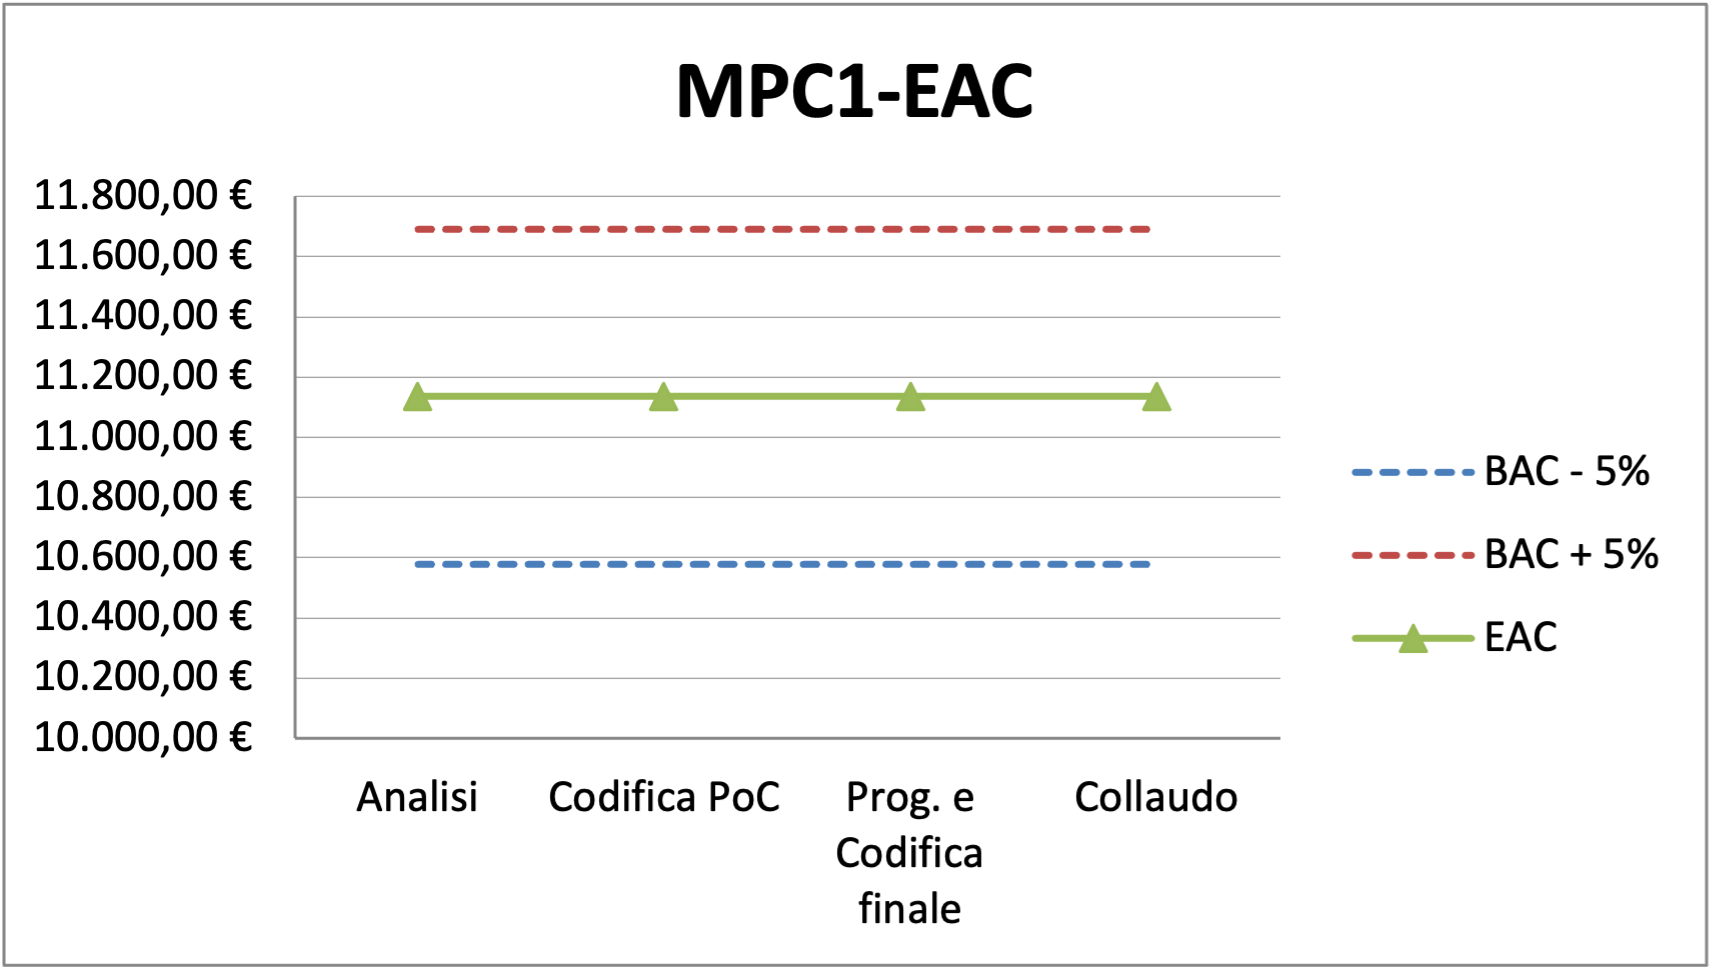
\includegraphics[width=0.8\textwidth]{images/MPC1-EAC.png}
    \caption{MPC1-EAC: Estimated At Completion}
\end{figure}
\noindent \textbf{Considerazioni RTB:} Si nota come la stima del costo totale (EAC) sia in linea con il budget inizialmente preventivato per entrambi i periodi di Analisi e Codifica del PoC. Si vuole dunque cercare di mantenere questo risultato anche per i prossimi periodi.

\vspace{0.5cm}

\noindent \textbf{Considerazioni PB:} Si è riusciti nell'obiettivo posto da questa metrica. La stima del costo totale, infatti, non ha mai subito variazioni nei periodi attraversati.

\newpage
\paragraph{MPC2-CV: Cost Variance}
\begin{figure}[h!] 
    \centering
    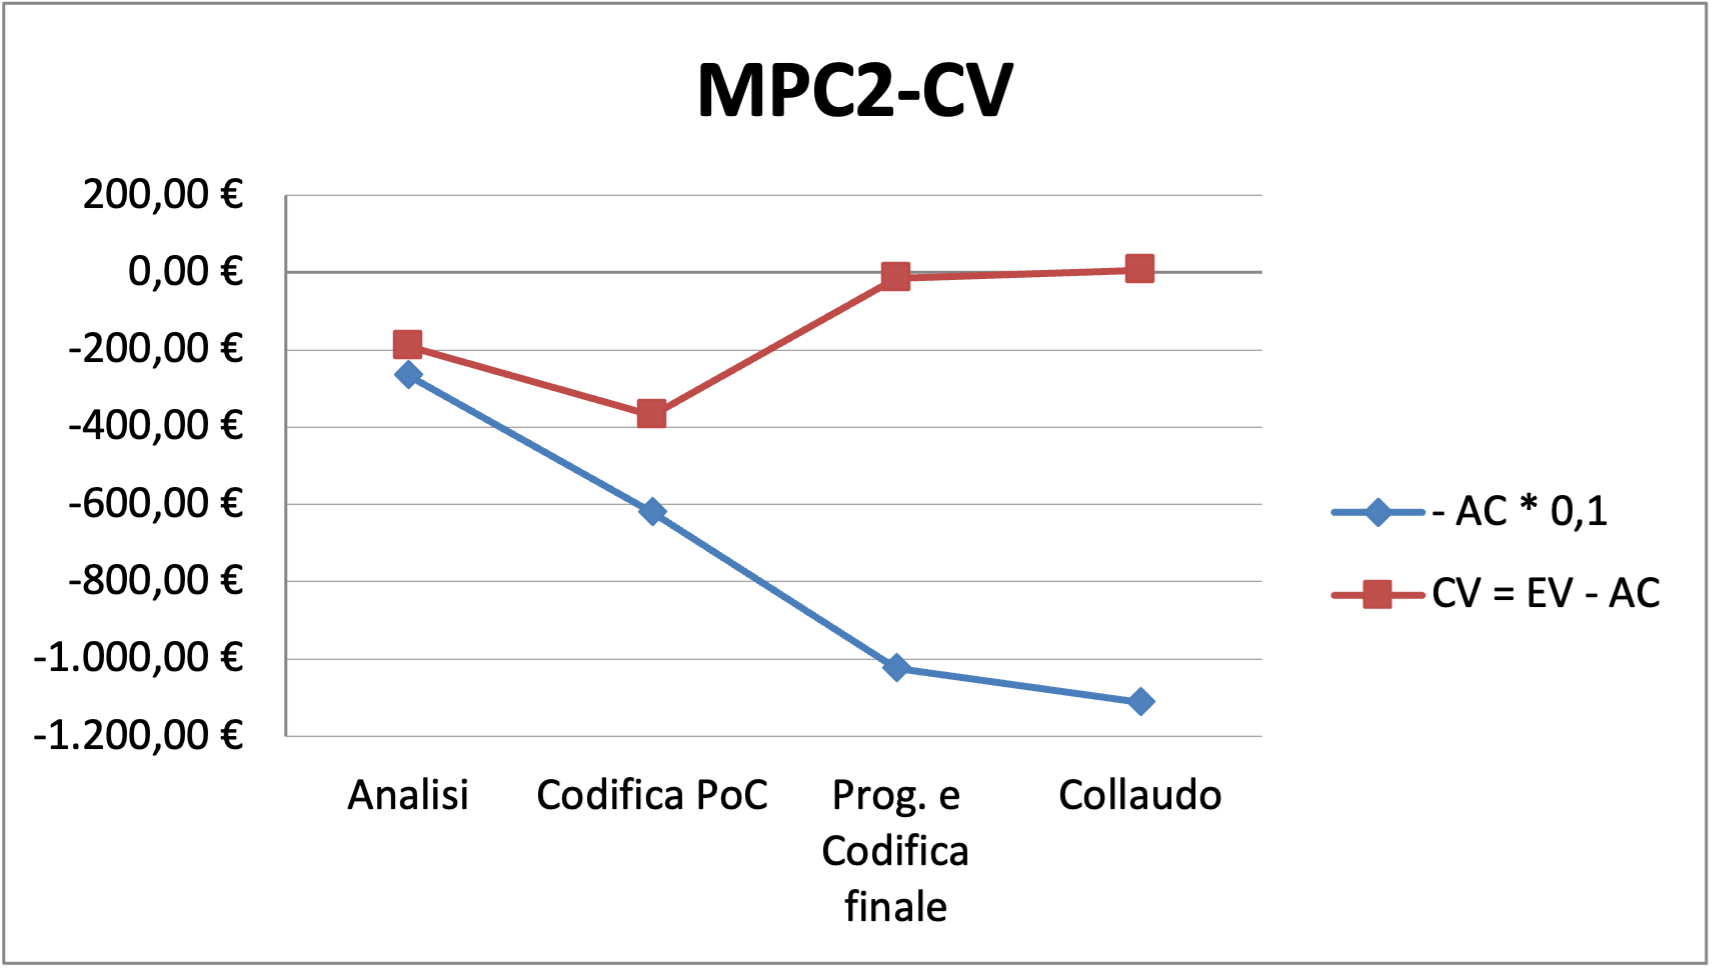
\includegraphics[width=0.8\textwidth]{images/MPC2-CV.png}
    \caption{MPC2-CV: Cost Variance}
\end{figure}
\noindent \textbf{Considerazioni RTB:} Pur rimanendo entro i limiti previsti dalle metriche, il Cost Variance (CV) non rispetta il valore ottimale, in quanto il valore delle attività realizzate è inferiore al costo sostenuto. Sarà dunque necessario attuare dei miglioramenti dal punto di vista produttivo, in modo che i costi per le attività siano ben giustificati.

\vspace{0.5cm}
\noindent \textbf{Considerazioni PB:} La fase di progettazione e codifica è risultata estremamente produttiva nonostante l'aumento sostanziale dei costi sostenuti, arrivando ad un valore ottimale per la metrica CV. Non sono state dunque necessarie azioni correttive. Il periodo di Collaudo ha visto confermare la stabilità della relazione tra costi e valore del prodotto. 


\paragraph{MPC3-SV: Schedule Variance}
\begin{figure}[h!]
    \centering
    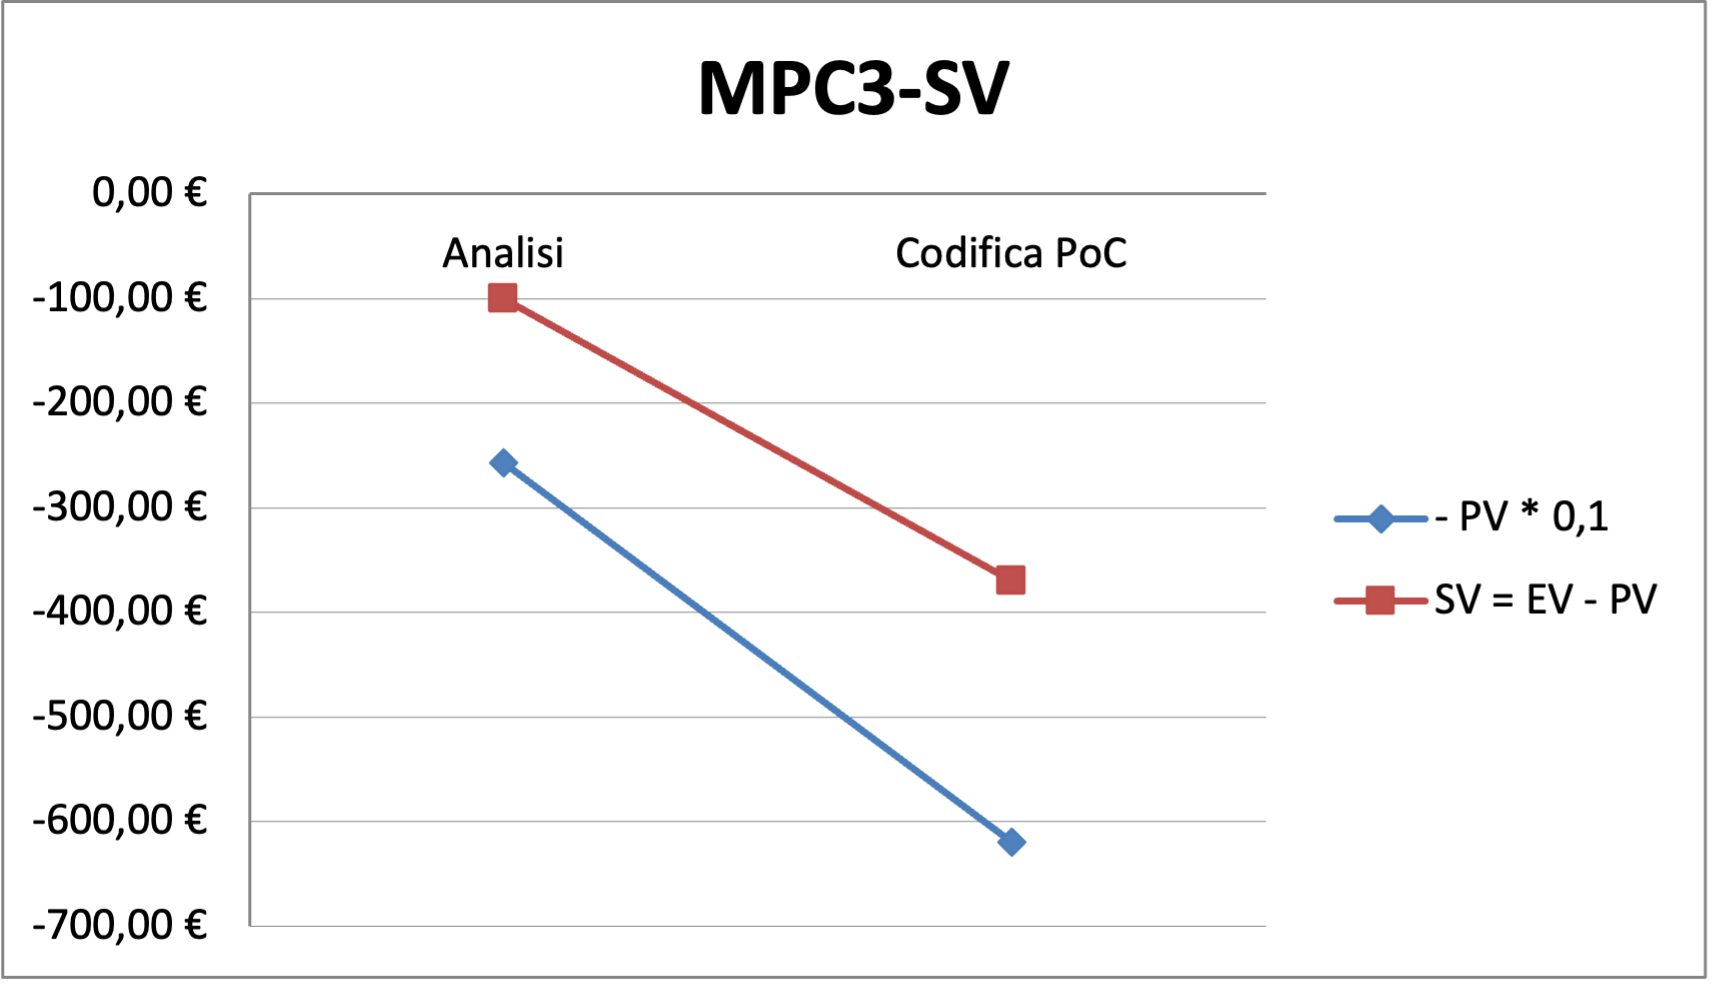
\includegraphics[width=0.8\textwidth]{images/MPC3-SV.png}
    \caption{MPC3-SV: Schedule Variance}
\end{figure}
\noindent \textbf{Considerazioni RTB:} Si nota come la Schedule Variance (SV) risulta avere un calo durante il periodo di progettazione e codifica del PoC, suggerendo quindi che ci sono stati dei ritardi rispetto alla pianificazione prevista. Il motivo di questi ritardi è dovuto allo studio delle nuove tecnologie che ha richiesto più tempo del previsto e alla sessione di esami che ha tolto del tempo allo svolgimento del progetto.

\vspace{0.5cm}
\noindent \textbf{Considerazioni PB:} L'accumulo di ritardi nella fase precedente ha provocato un aumento della produttività del gruppo, riuscendo a risollevare, nella fase di Progettazione e codifica, la metrica SV fino a valori accettabili. Si è riusciti a mantenere costante il livello di produttività anche nella fase di Collaudo che, anzi, è stata ancora più positiva della precedente, arrivando ad ottenere valori ottimali per la metrica SV.

\paragraph{MPC4-BV: Budget Variance}
\begin{figure}[h!] 
    \centering
    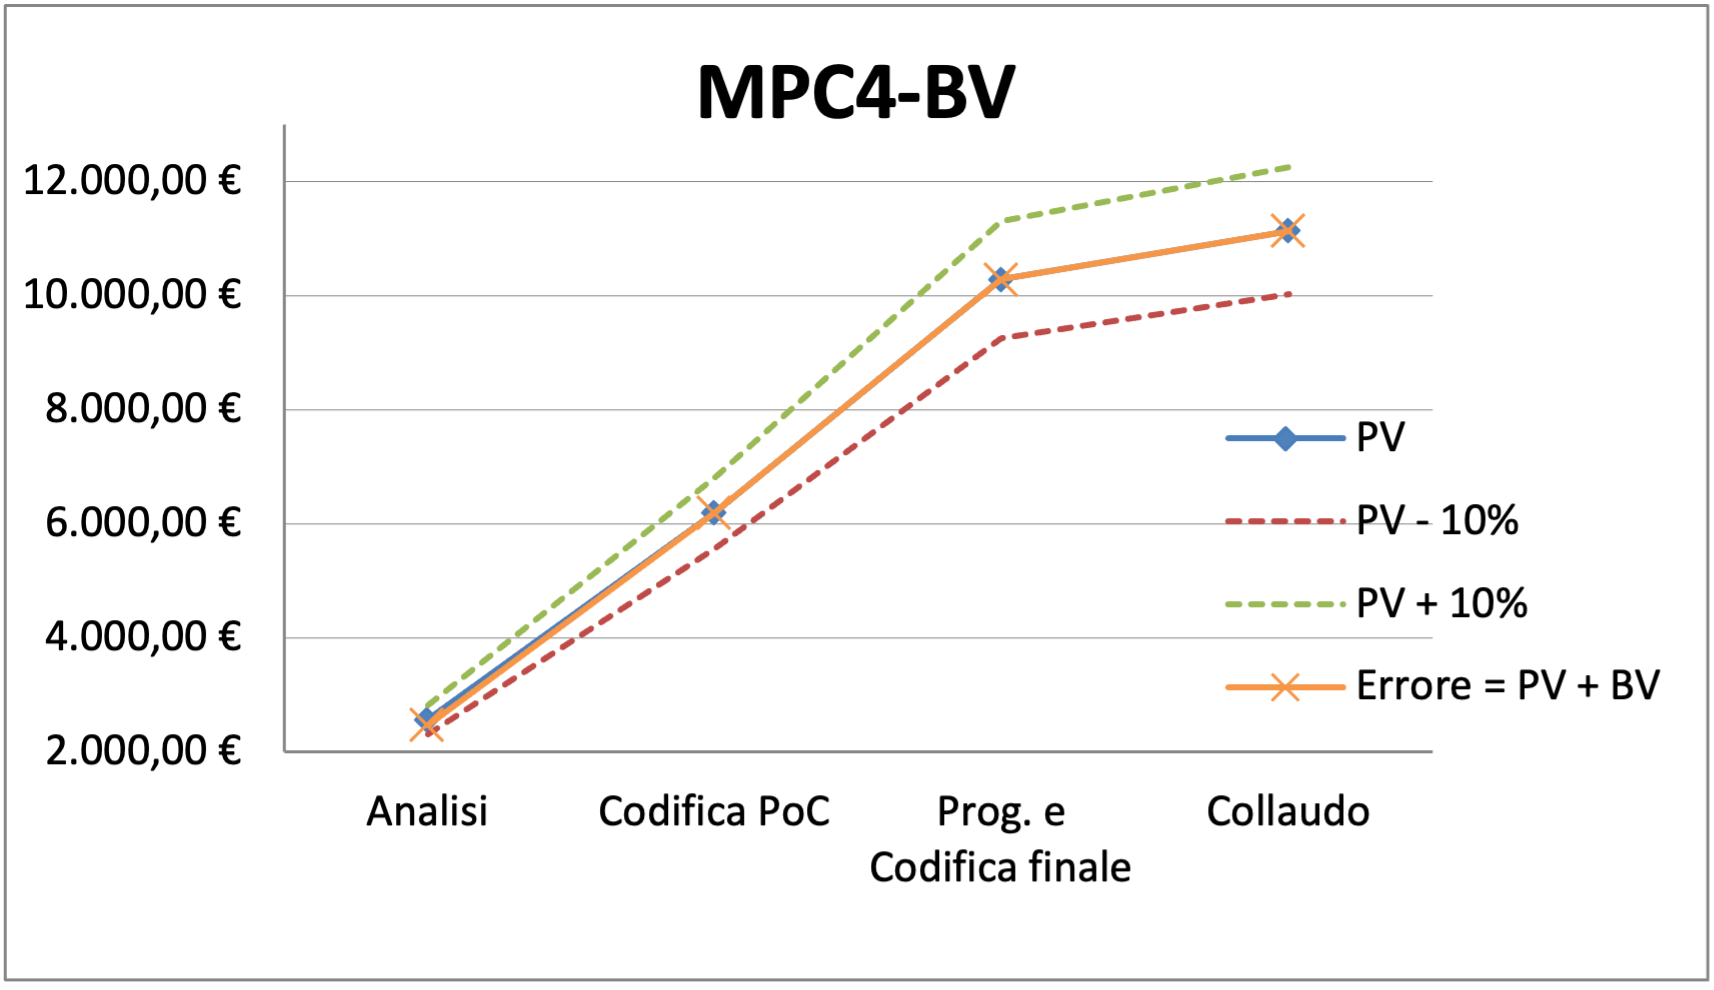
\includegraphics[width=0.8\textwidth]{images/MPC4-BV.png}
    \caption{MPC4-BV: Budget Variance}
\end{figure}
\noindent \textbf{Considerazioni RTB:} Si nota come sostanzialmente l'errore rimane pressoché nullo, a significare che i costi della pianificazione iniziale corrispondono quasi completamente a quelli effettivi. Si cerca di dunque di mantenere questa linea anche per i prossimi periodi.

\vspace{0.5cm}
\noindent \textbf{Considerazioni PB:} Anche in queste fasi l'errore di previsione di costi rimane pressochè nullo. I ritardi accumulati in fase RTB non hanno dunque influenzato i costi, che rimangono in linea con quelli pianificati.

\paragraph{MPC5-PV: Planned Value}
\begin{figure}[H]
    \centering
    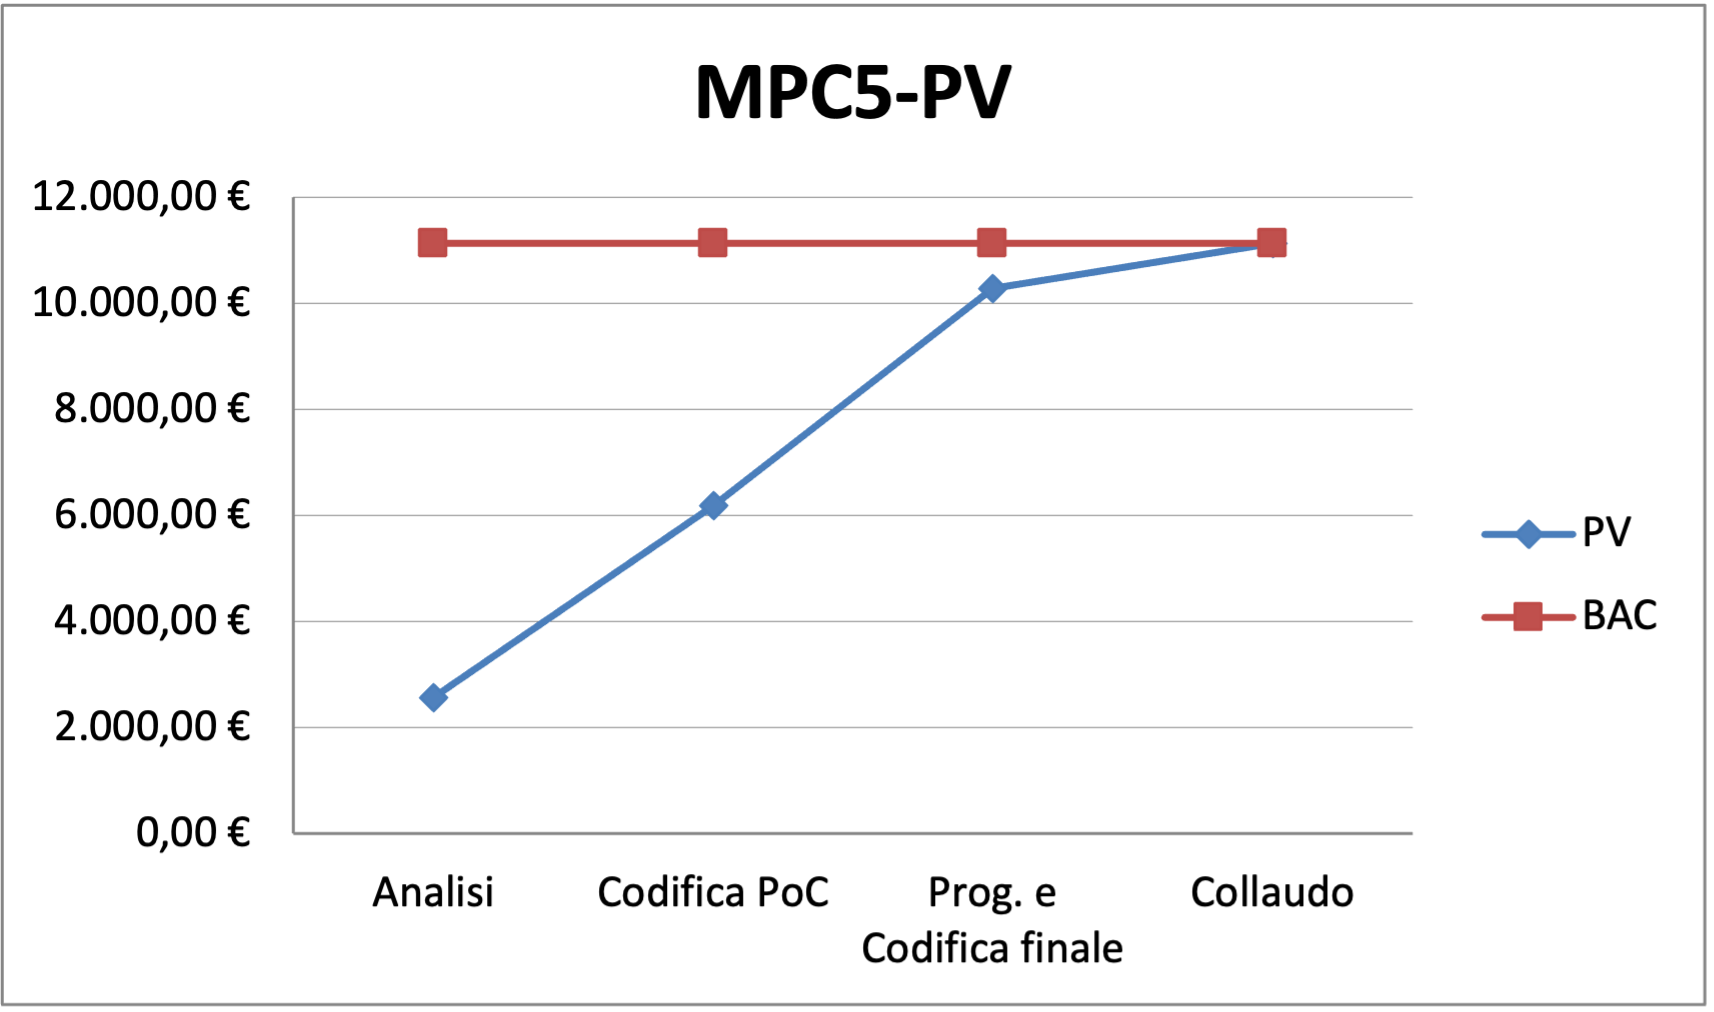
\includegraphics[width=0.8\textwidth]{images/MPC5-PV.png}
    \caption{MPC5-PV: Planned Value}
\end{figure}
\noindent \textbf{Considerazioni RTB:} Si deduce dal grafico che i costi sostenuti per i periodi di Analisi e Codifica del PoC rimangono inferiori a quelli previsti totalmente per la realizzazione del progetto. Ovviamente si ha un incremento in questi costi dovuti all'avanzare del progetto, ma rimane comunque controllato.

\vspace{0.5cm}
\noindent \textbf{Considerazioni PB:} 
Per la fase di Progettazione e codifica finale si è previsto un sostanziale consumo di risorse che però rimane sotto al limite massimo previsto (corrispondente al BAC). Pertanto, non sono state effettuate azioni correttive. Per quanto riguarda la fase di Collaudo, il budget rimanente è scarso ma la previsione finale si allinea a quella iniziale. 

\paragraph{MPC6-AC: Actual Cost}
\begin{figure}[h!] 
    \centering
    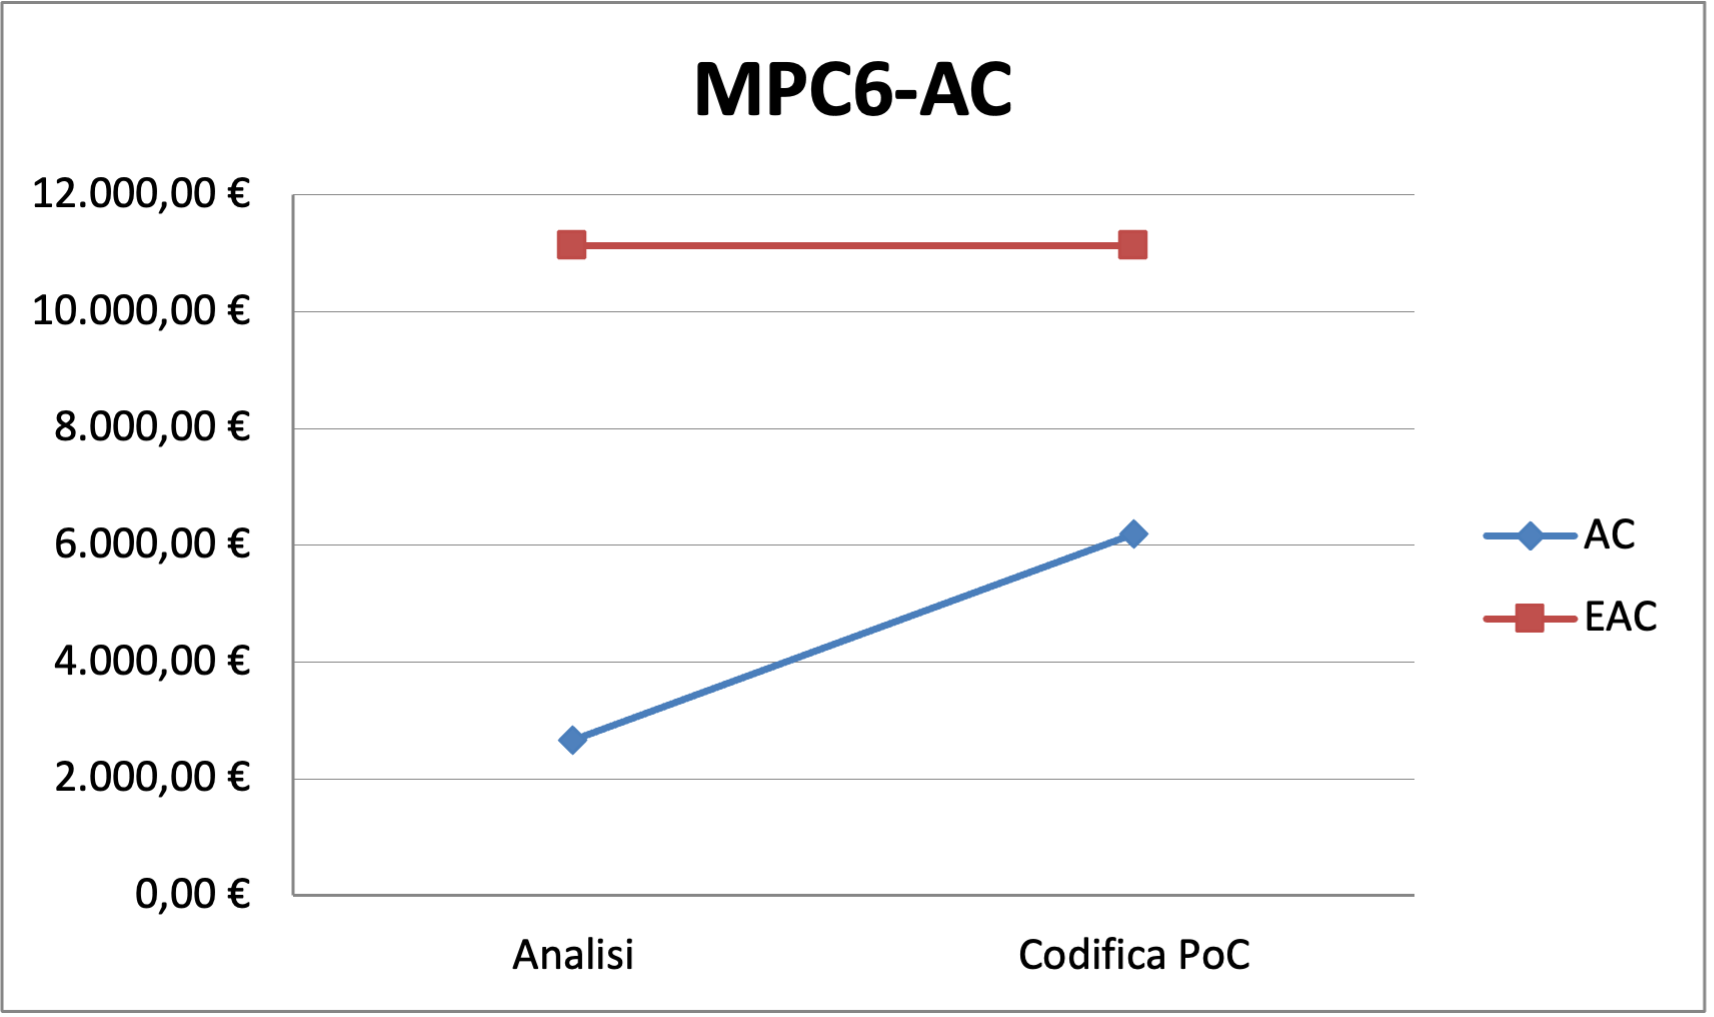
\includegraphics[width=0.8\textwidth]{images/MPC6-AC.png}
    \caption{MPC6-AC: Actual Cost}
\end{figure}
\noindent \textbf{Considerazioni RTB:} Si osserva che l’Actual Cost (AC) mostra un incremento, come naturale con il progredire del progetto, ma rimane comunque sotto la soglia dell'Estimated at Completion (EAC). 

\vspace{0.5cm}
\noindent \textbf{Considerazioni PB:} Nella fase di progettazione e codifica si è verificato un grande consumo di risorse. Tuttavia, al termine del periodo, l'Actual Cost (AC) non supera comunque la soglia dell'Estimated At Completion (EAC).


\paragraph{MPC7-EV: Earned Value}
\begin{figure}[h!] 
    \centering
    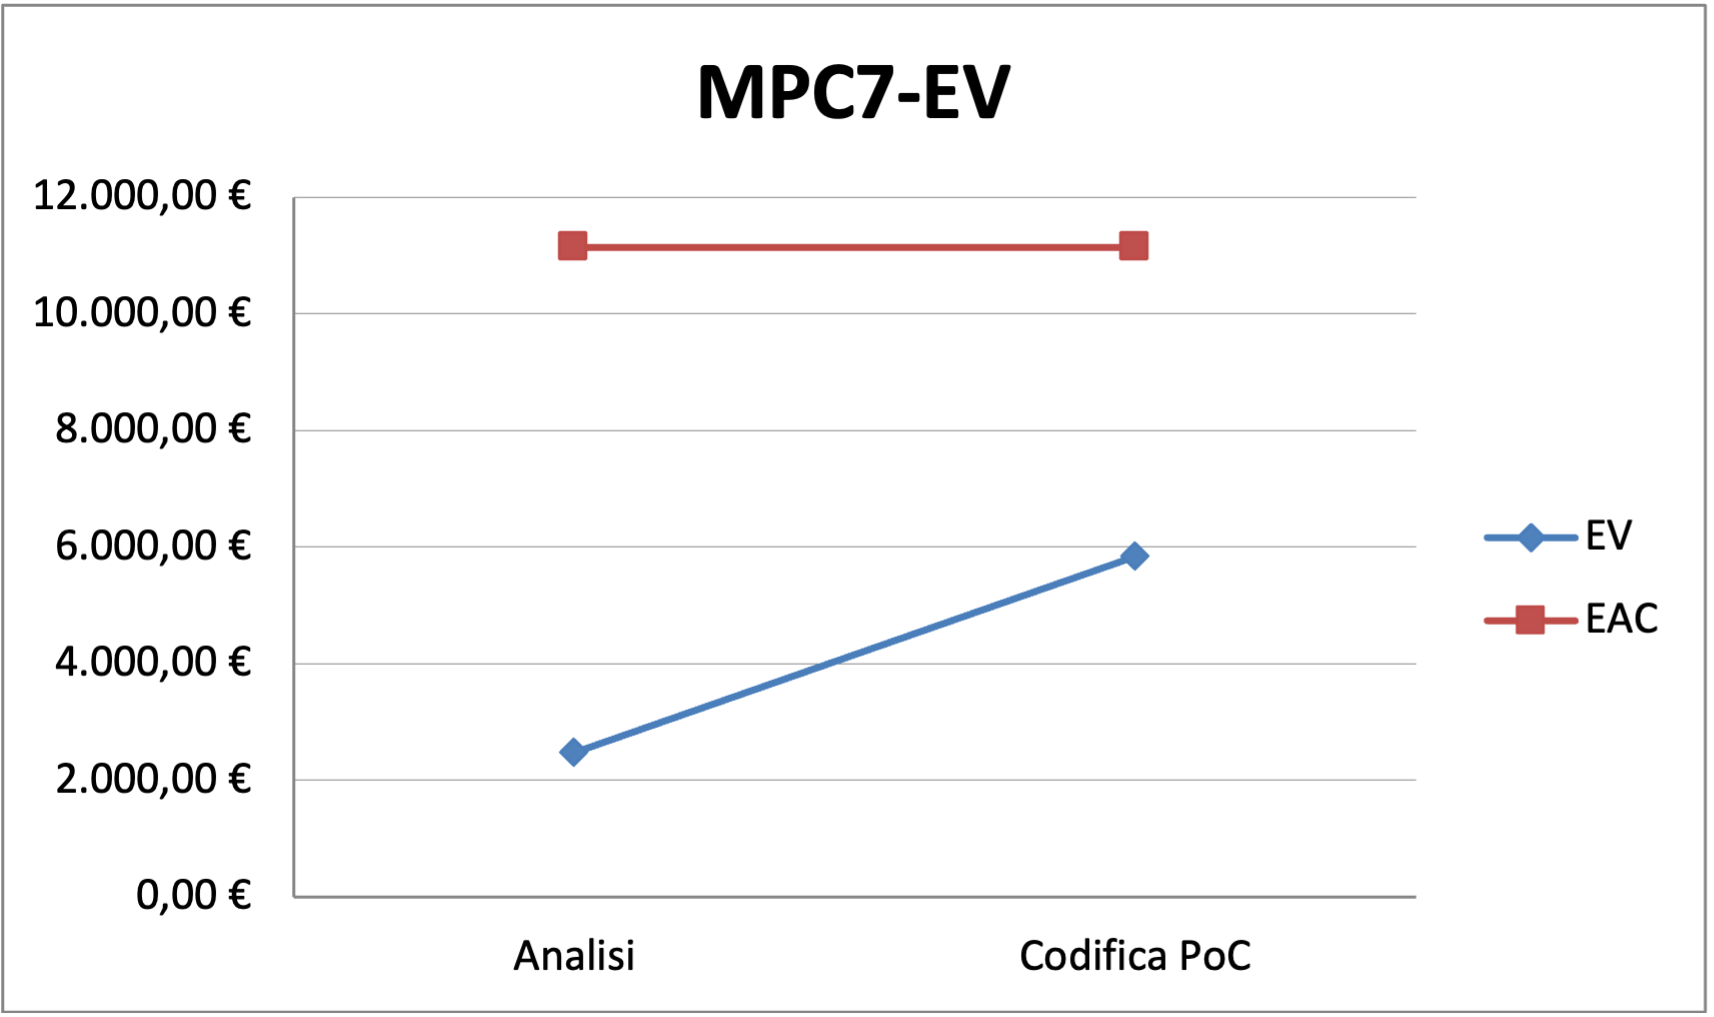
\includegraphics[width=0.8\textwidth]{images/MPC7-EV.png}
    \caption{MPC7-EV: Earned Value}
\end{figure}
\noindent \textbf{Considerazioni RTB:} Si nota che l'Earned Value (EV) rimane minore dell'Estimated at Completion (EAC), a significare che il valore effettivo delle attività di progetto svolte fino all'RTB non sfora i costi pianificati per l'intero progetto, seppur ovviamente aumenta con il susseguirsi dei vari periodi.

\vspace{0.5cm}
\noindent \textbf{Considerazioni PB:} Nella fase di progettazione e codifica ci si è avvicinati spaventosamente al limite di costi previsti. Nella fase successiva di Collaudo si è tenuto conto della scarsità di capitale rimanente e si è riusciti a rientrare entro i limiti della metrica.

\subsubsection{Qualità di processo - Sviluppo} \label{sec:sviluppo}
Si noti che le seguenti metriche saranno analizzate soltanto per il periodo di Progettazione e codifica finale in quanto lo sviluppo finale del prodotto è avvenuto in questo periodo.

\paragraph{MPC8-SFINp: Structural Fan-In}  
Il design del prodotto, meglio descritto nel documento \textit{Specifica Tecnica}, consultabile nella sezione \ref{sec:riferimenti_esterni}, prevede un alto utilizzo delle procedure definite nello store da parte dei componenti grafici. Il riutilizzo di codice è dunque molto alto e rende la metrica SFINp soddisfatta.

\paragraph{MPC9-SFOUTp: Structural Fan-Out}
I componenti grafici non hanno alcuna dipendenza tra di loro, mentre la parte di store è intrinsecamente interdipendente per via dei design pattern utilizzati. La metrica è dunque da ritenersi soddisfatta.

\newpage
\paragraph{MPC10-CCH: Code Churn}

\textbf{Nota:} Si noti che sono stati presi in considerazione solamente i componenti soggetti ad un numero sostanziale di modifiche.

\begin{figure}[h!] 
    \centering
    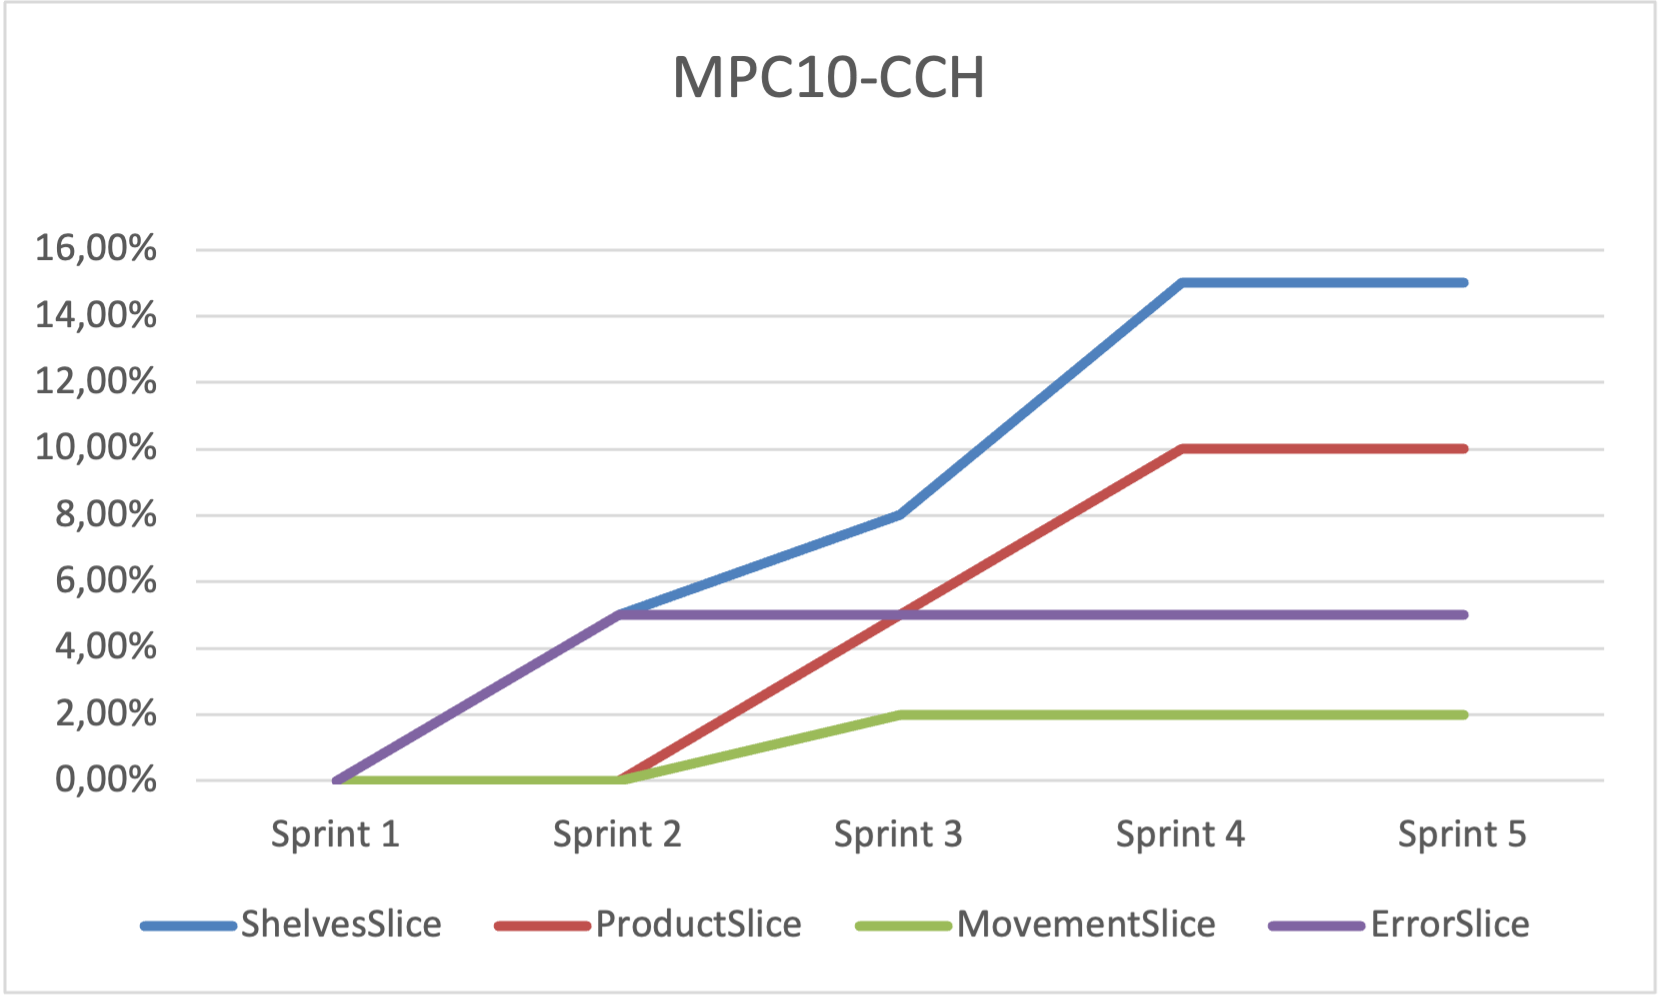
\includegraphics[width=0.8\textwidth]{images/MPC10-CCH.png}
    \caption{MPC10-CCH: Code Churn}
\end{figure}

\noindent \textbf{Considerazioni:} Gli Sprint 1, 2 e 3 sono stati soggetti ad un modesto numero di modifiche, causando cambiamenti di codice che hanno rallentato momentaneamente lo sviluppo. Questa esperienza ha causato un ritorno di attenzione sull'UML del progetto, modificandolo ed aggiornandolo in maniera dettagliata. Gli sprint successivi sono infatti più stabili.


\paragraph{MPC11-NB: Number of Bugs}
\begin{figure}[h!] 
    \centering
    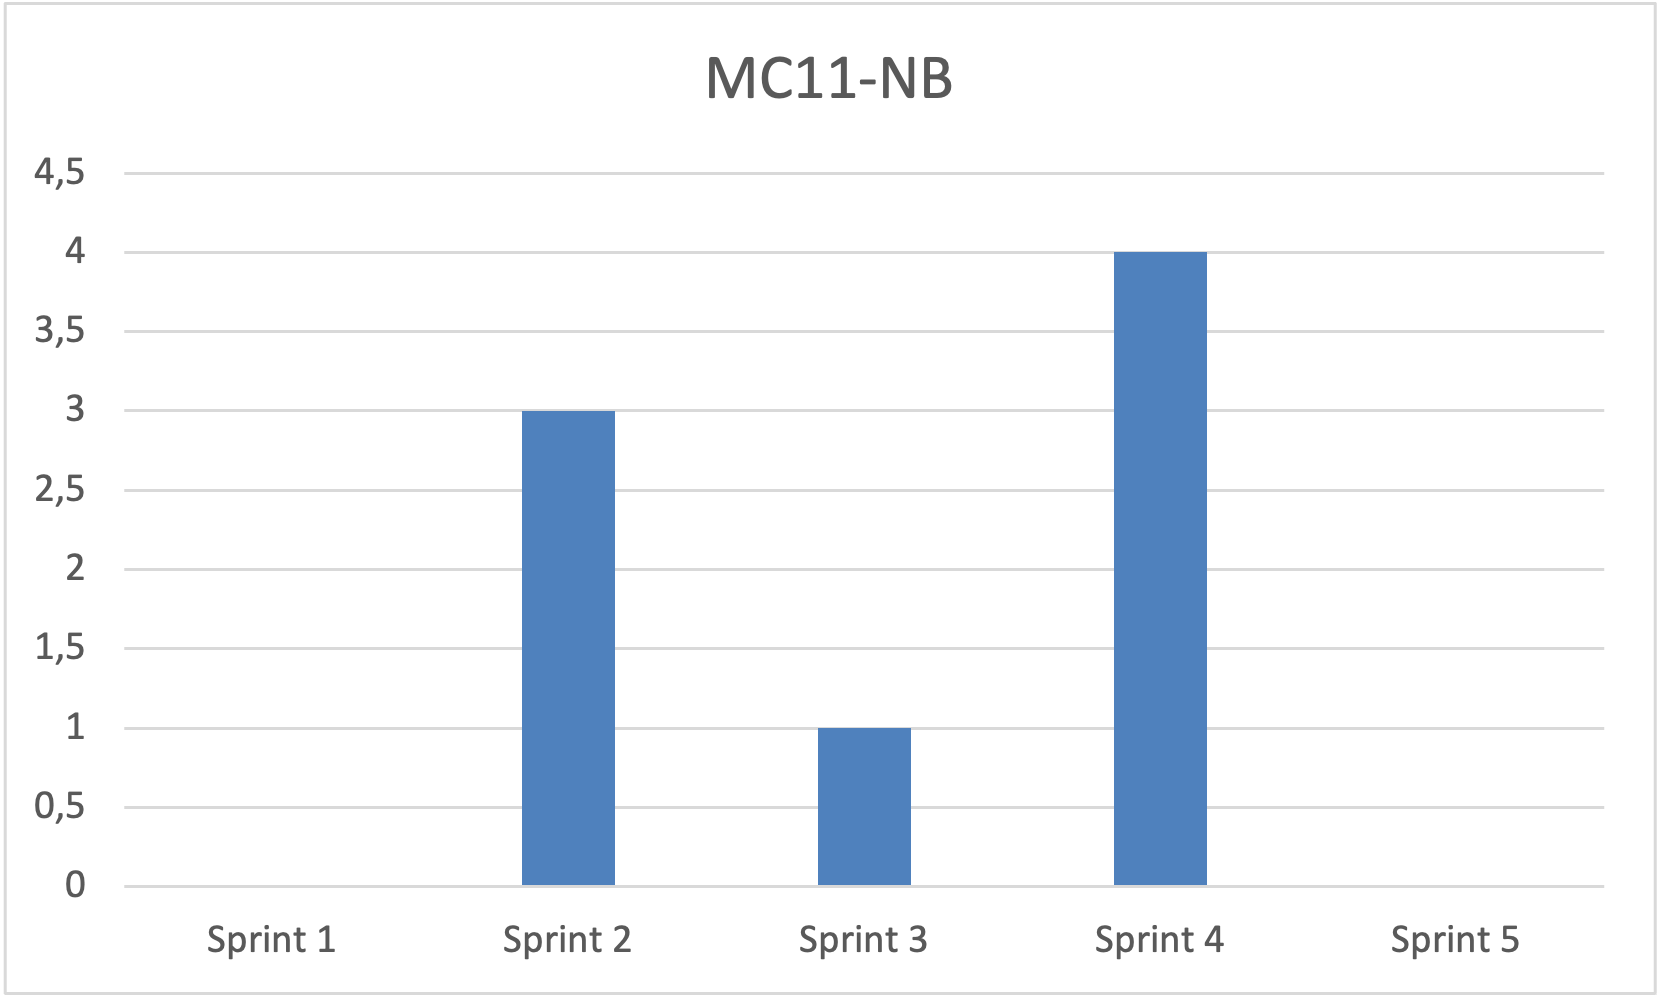
\includegraphics[width=0.8\textwidth]{images/MPC11-NB.png}
    \caption{MPC11-NB: Number of Bugs}
\end{figure}

\noindent \textbf{Considerazioni:} Durante lo sviluppo del codice sono stati rilevati e corretti alcuni bug. Il prodotto finale non contiene bug rilevati. La metrica è dunque soddisfatta in maniera ottimale.

\paragraph{MPC12-CC: Cyclomatic Complexity}

Di seguito sono analizzati in ordine decrescente i valori di Cyclomatic Complexity (CC) dei componenti del prodotto:

\begin{figure}[h!] 
    \centering
    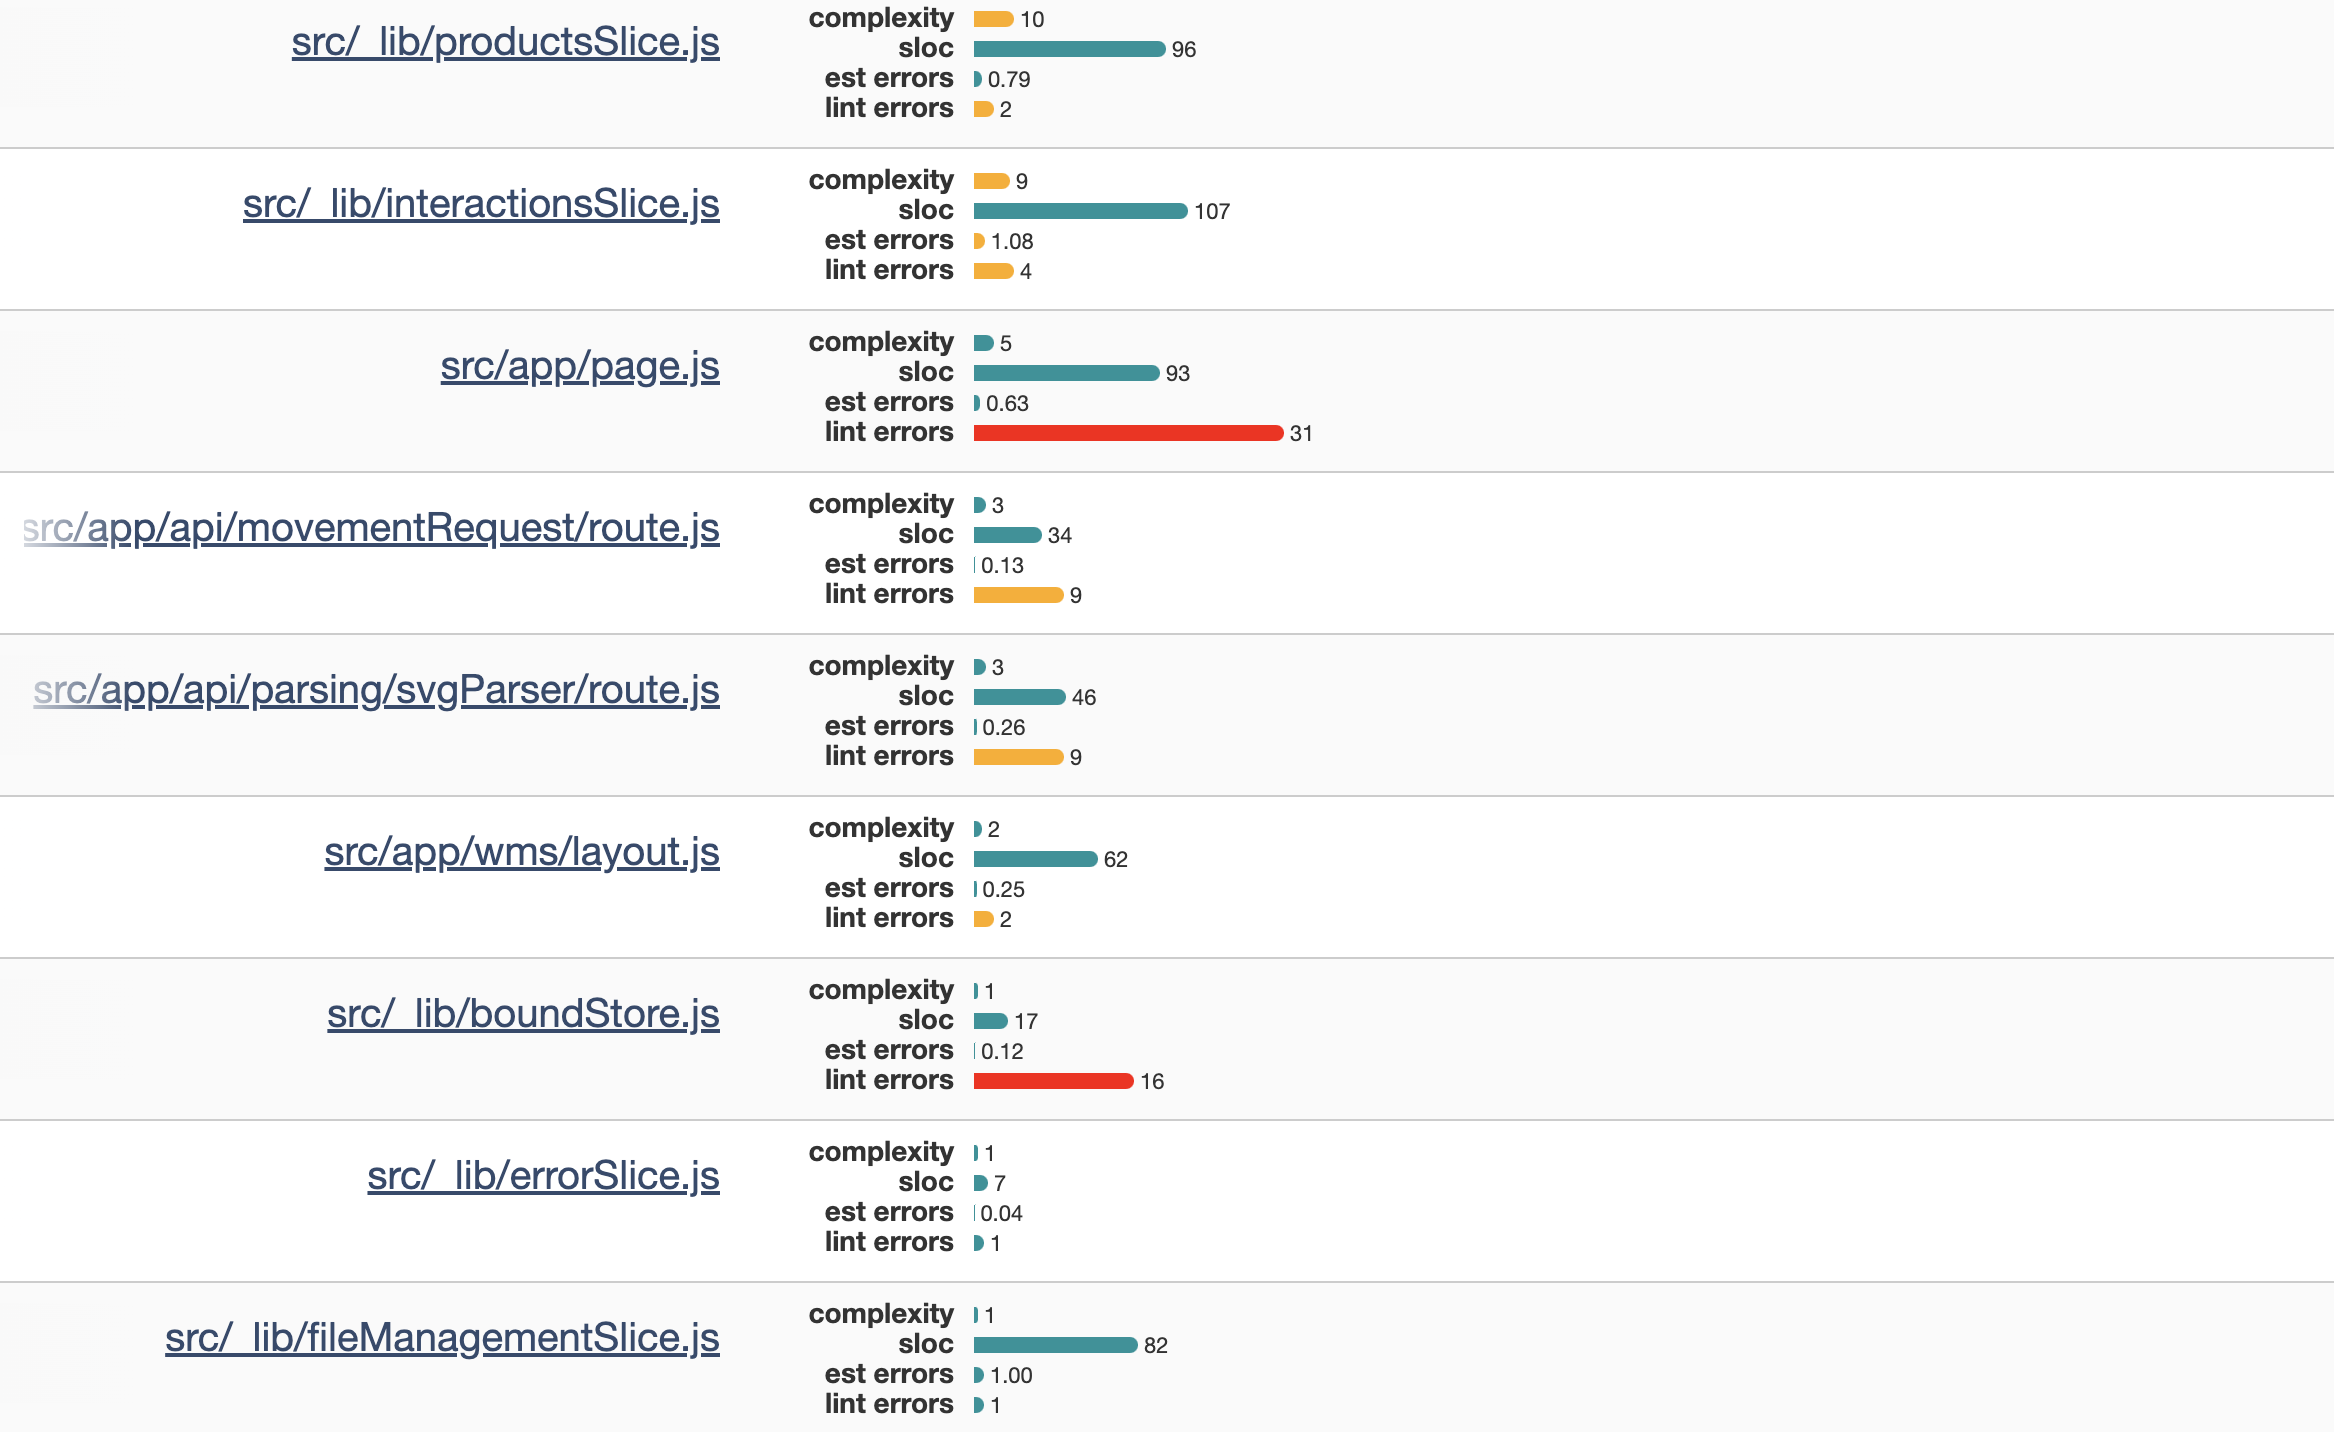
\includegraphics[width=0.9\textwidth]{images/MPC12-CC.png}
    \caption{MPC12-CC: Cyclomatic Complexity}
\end{figure}

\noindent \textbf{Considerazioni:} Come si nota, il valore di complessità massimo è raggiunto in ProductSlice ma è comunque compreso tra i valori ottimali scelti per questa metrica.

\newpage

\subsection{Processi di supporto} \label{sec:processi_di_supporto}
Di seguito sono visualizzati i grafici e i resoconti relativi alle metriche dei processi di supporto.
\subsubsection{Qualità di processo - Documentazione}
\paragraph{MPC13-EOD: Errori ortografici per documento}
\begin{figure}[h!] 
    \centering
    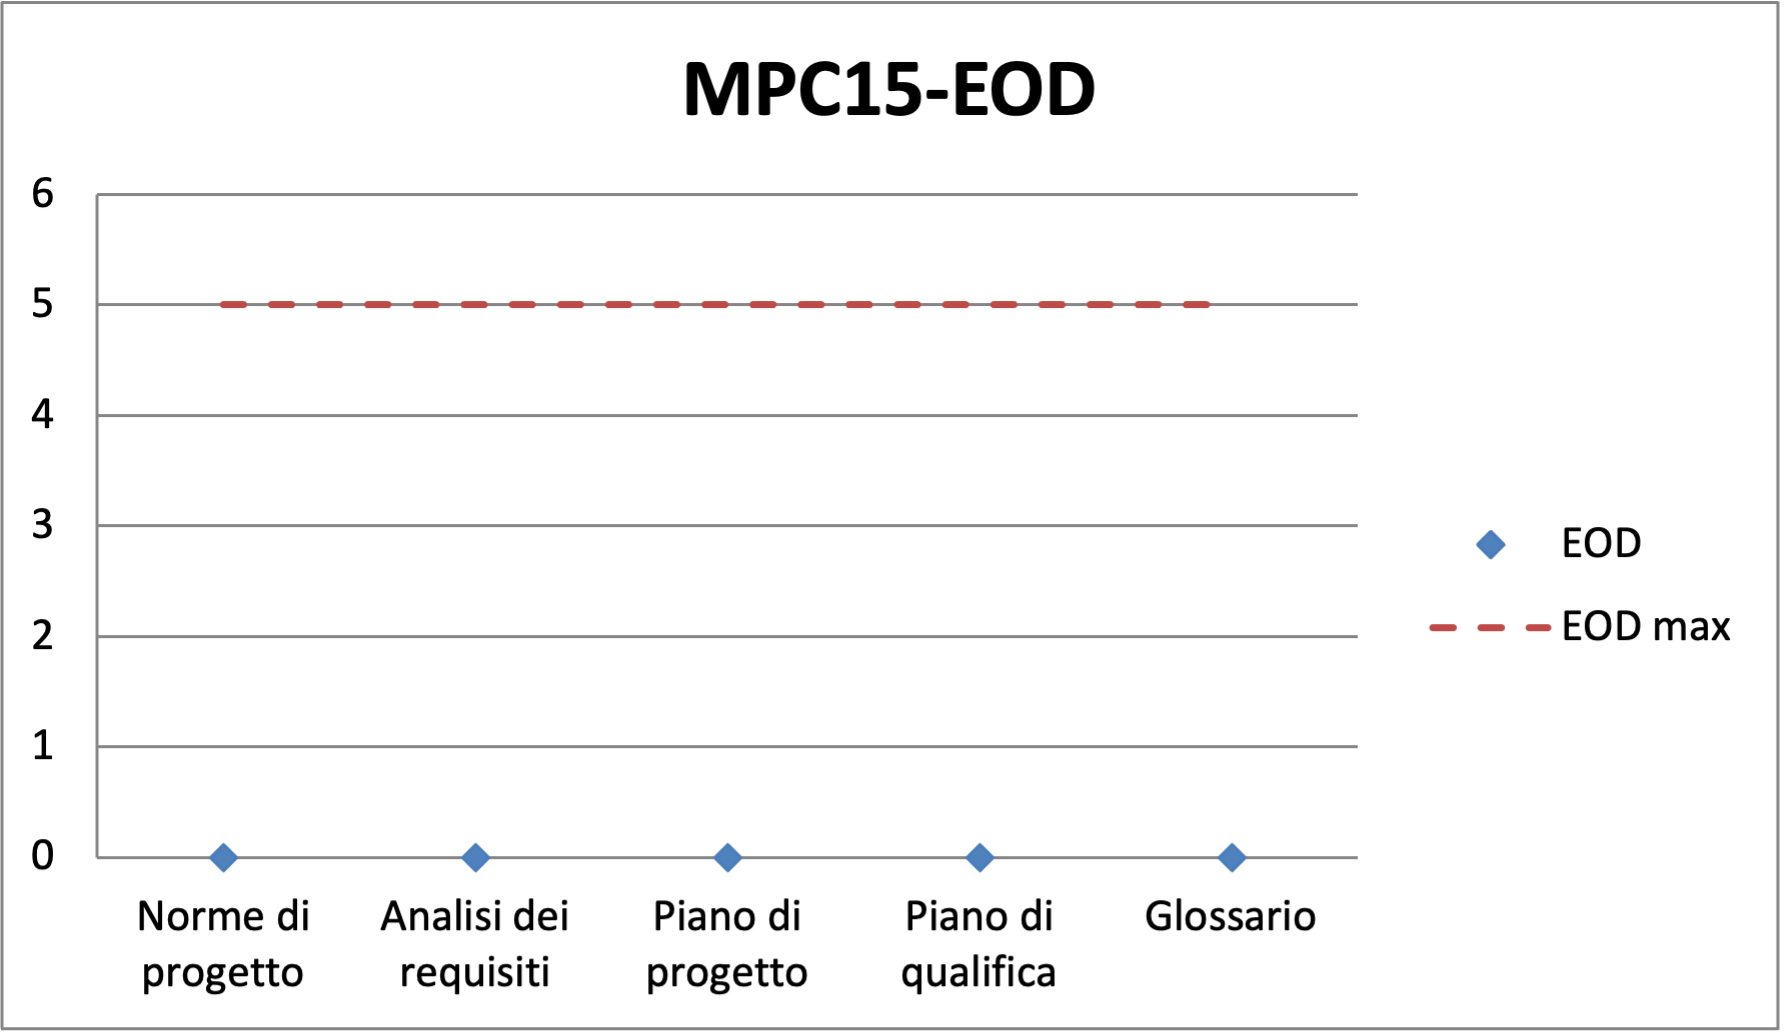
\includegraphics[width=0.8\textwidth]{images/MPC13-EOD.png}
    \caption{MPC13-EOD: Errori ortografici per documento}
\end{figure}
\noindent \textbf{Considerazioni:} Il gruppo si è impegnato a mantenere una documentazione priva di errori ortografici. La metrica è dunque soddisfatta ina maniera ottimale.


\paragraph{MPC14-IG: Indice Gulpease}
\begin{figure}[h!]
    \centering
    \begin{subfigure}[b]{0.49\textwidth}
        \centering
        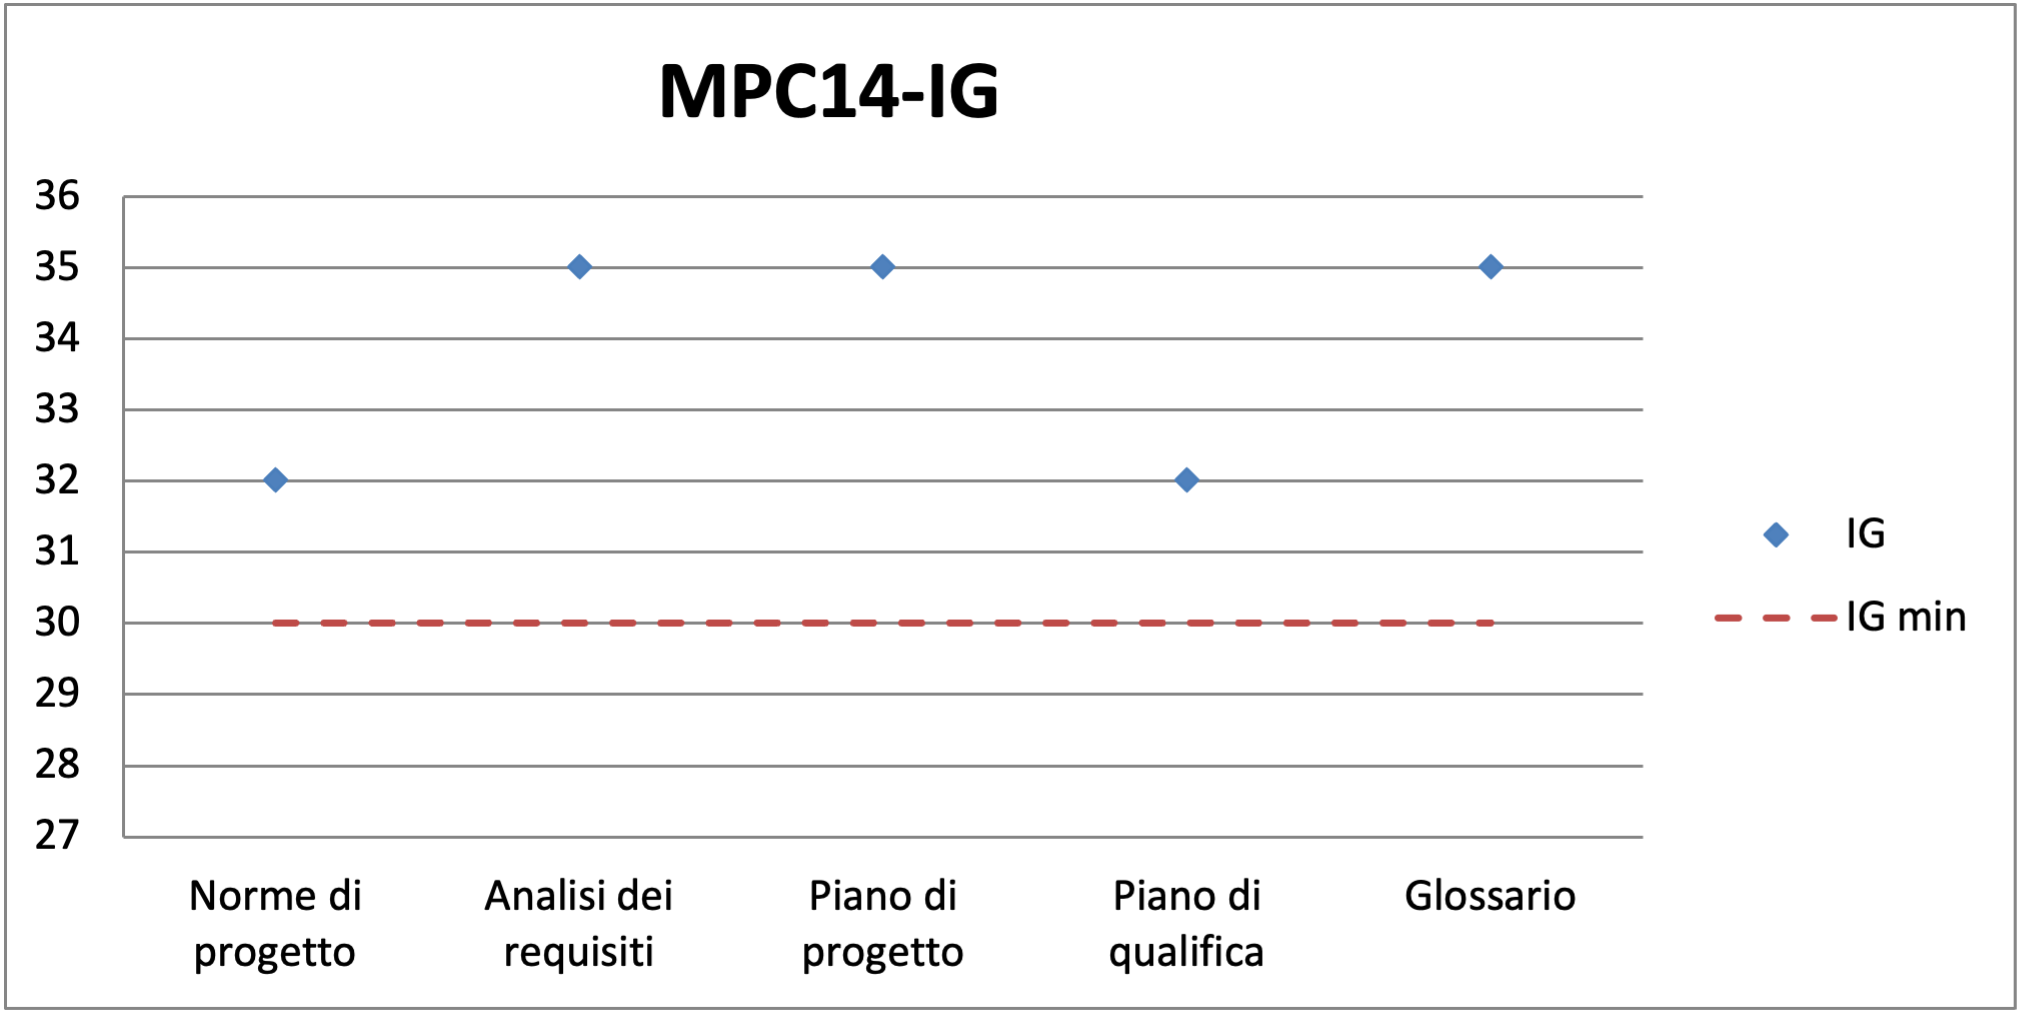
\includegraphics[width=\textwidth]{images/MPC14-EODrtb.png}
        \caption{MPC14-IG RTB}
        \label{fig:image1}
    \end{subfigure}
    \hfill
    \begin{subfigure}[b]{0.49\textwidth}
        \centering
        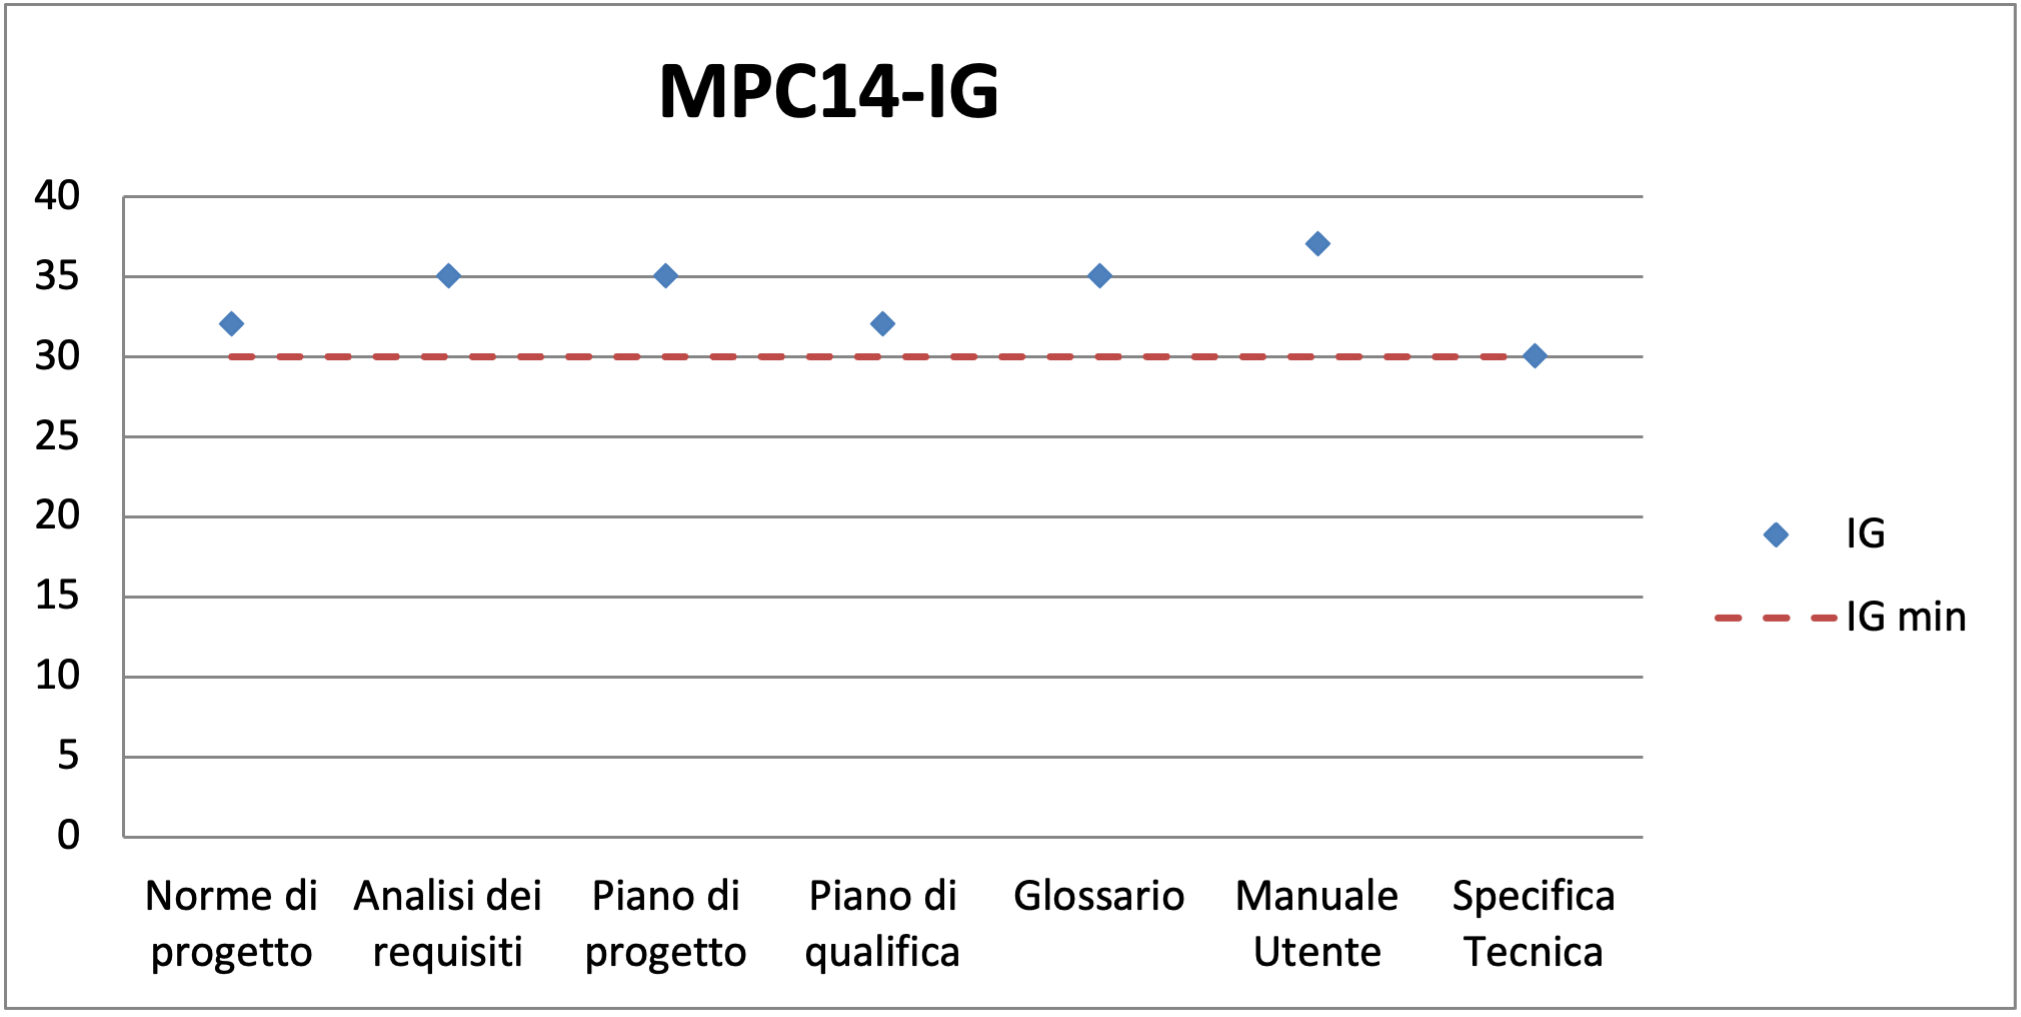
\includegraphics[width=\textwidth]{images/MPC14-IG.png}
        \caption{MPC14-IG PB}
        \label{fig:image2}
    \end{subfigure}
    \caption{MPC14-1G Indice Gulpease}
    \label{fig:whole_figure}
\end{figure}

\noindent \textbf{Considerazioni RTB:} Si osserva come l'indice di Gulpease rimane accettabile per tutti i documenti, tuttavia non raggiunge mai l'ottimalità. Il gruppo, pertanto, dovrà impegnarsi ad utilizzare termini meno tecnici (se possibile) e strutturare i periodi in maniera più semplice.

\vspace{0.5cm}
\noindent \textbf{Considerazione PB:} La natura tecnica della documentazione prodotta non ha permesso un miglioramento netto ma i documenti soddisfano i valori minimi.

\subsubsection{Qualità di processo - Accertamento della qualità}
\paragraph{MPC15-MS: Metriche soddisfatte} \label{sec:accertamento delle qualita}

\noindent \textbf{Considerazioni RTB:}
Le metriche prese in considerazione in questa fase sono:
\begin{itemize}
    \item MPC1-EAC \colorbox{green}{Soddisfatta} 
    \item MPC2-CV \colorbox{green}{Soddisfatta} 
    \item MPC3-SV \colorbox{green}{Soddisfatta}
    \item MPC4-BV \colorbox{green}{Soddisfatta} 
    \item MPC5-PV \colorbox{green}{Soddisfatta} 
    \item MPC6-AC \colorbox{green}{Soddisfatta} 
    \item MPC7-EV \colorbox{green}{Soddisfatta} 
    \item MPC13-EOD \colorbox{green}{Soddisfatta}
    \item MPC14-IG \colorbox{green}{Soddisfatta}
\end{itemize}

\noindent La percentuale di metriche soddisfatte (MPC15-MS) equivale al \textbf{100\%}. Pertanto, possiamo dire che si è raggiunto un livello di ottimalità per questa metrica.

\bigskip
\noindent \textbf{Considerazioni PB:}
Le metriche prese in considerazione in questa fase sono:
\begin{itemize}
    \item MPC1-EAC \colorbox{green}{Soddisfatta};
    \item MPC2-CV \colorbox{green}{Soddisfatta};
    \item MPC3-SV \colorbox{green}{Soddisfatta};
    \item MPC4-BV \colorbox{green}{Soddisfatta};
    \item MPC5-PV \colorbox{green}{Soddisfatta};
    \item MPC6-AC \colorbox{green}{Soddisfatta};
    \item MPC7-EV \colorbox{green}{Soddisfatta};
    \item MPC8-SFINp \colorbox{green}{Soddisfatta};
    \item MPC9-SFOUTp \colorbox{green}{Soddisfatta};
    \item MPC10-CCH \colorbox{green}{Soddisfatta};
    \item MPC11-NB \colorbox{green}{Soddisfatta};
    \item MPC12-CC \colorbox{green}{Soddisfatta};
    \item MPC13-EOD \colorbox{green}{Soddisfatta};
    \item MPC14-IG \colorbox{green}{Soddisfatta};
    \item MPC16-CCV \colorbox{green}{Soddisfatta}.
    \item MPD17-TP \colorbox{green}{Soddisfatta};
    \item MPD1-ROB\colorbox{green}{Soddisfatta};
    \item MPD2-RDE\colorbox{green}{Soddisfatta};
    \item MPD3-ART \colorbox{green}{Soddisfatta};
    \item MPD4-PC \colorbox{green}{Soddisfatta};
    \item MPD5-CFO \colorbox{green}{Soddisfatta};
    \item MPD6-PPT \colorbox{green}{Soddisfatta};
\end{itemize}
\noindent La percentuale di metriche soddisfatte (MPC15-MS) equivale al \textbf{100\%}. Pertanto, possiamo dire che si è raggiunto un livello di ottimalità per questa metrica.


\subsubsection{Qualità di processo - Verifica}
\paragraph{MPC16-CCV: Code Coverage}
\textbf{Nota:} La scrittura dei test è iniziata parallelamente alla codifica, dunque nel seguente grafico sono presi in considerazione gli sprint di Progettazione e codifica e quelli di Collaudo.
\begin{figure}[h!] 
    \centering
    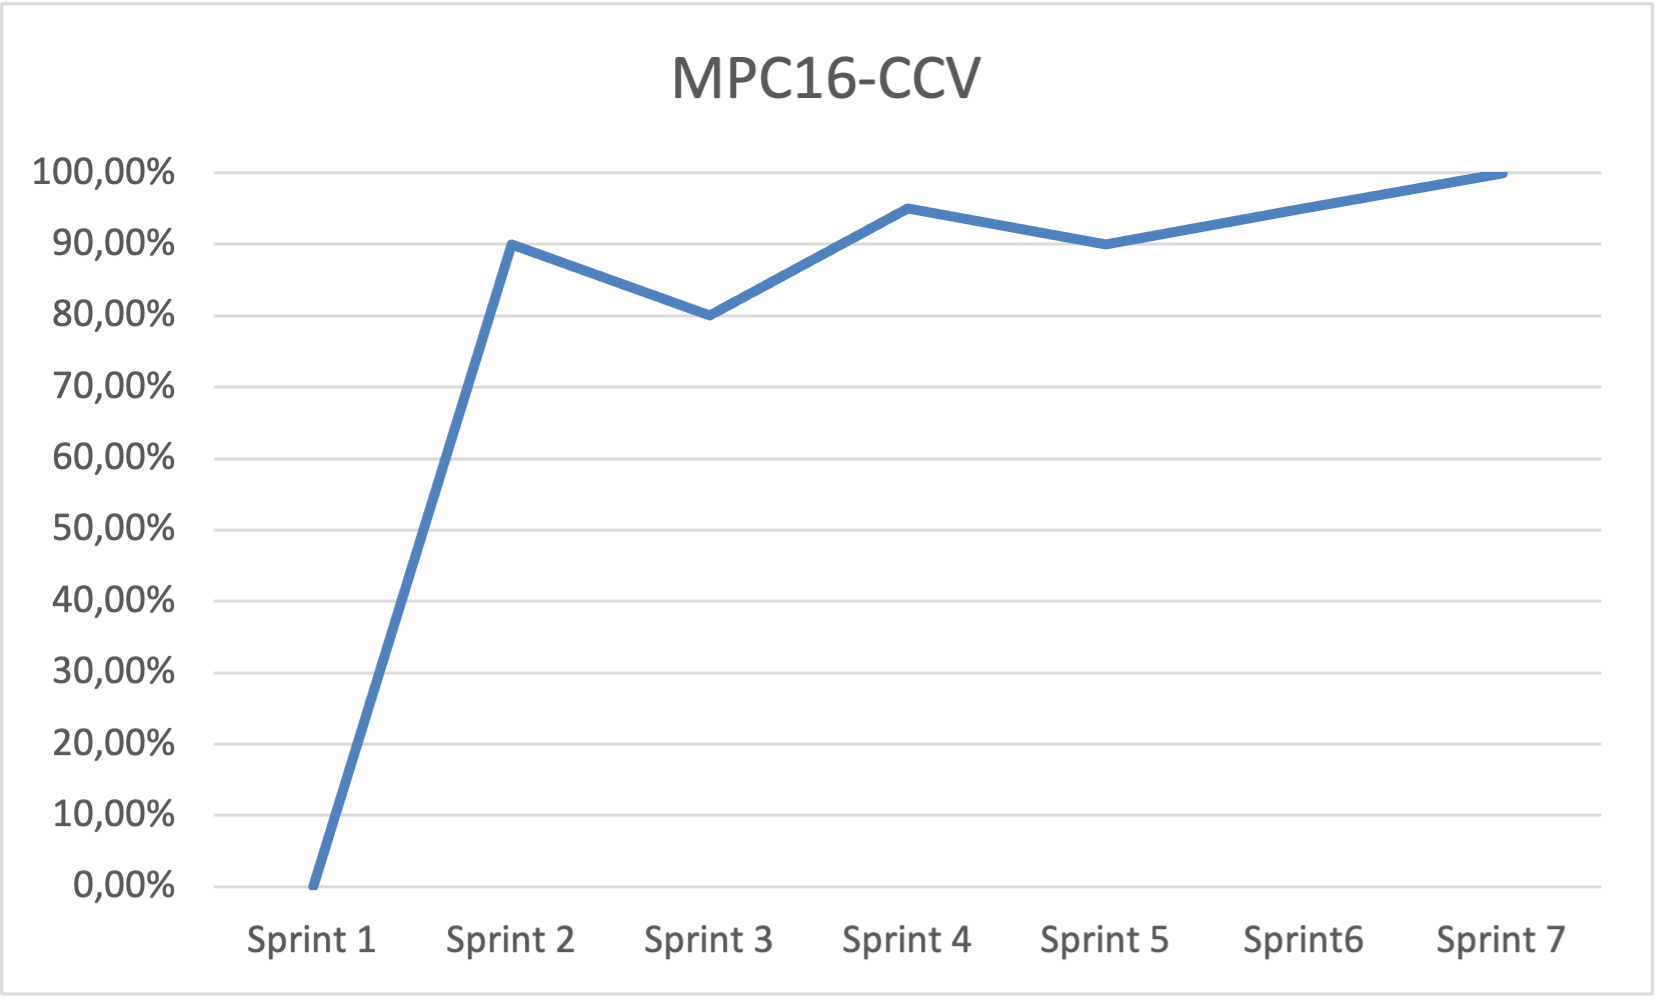
\includegraphics[width=0.8\textwidth]{images/MPC16-CCV.png}
    \caption{MPC16-CCV: Code Coverage}
\end{figure}

\noindent \textbf{Considerazioni:} La percentuale di Code Coverage è sempre stata elevata grazie ad una parallelizzazione del lavoro di Verificatori e Programmatori.

\paragraph{MPC17-TP: Test Passed}
\begin{figure}[H] 
    \centering
    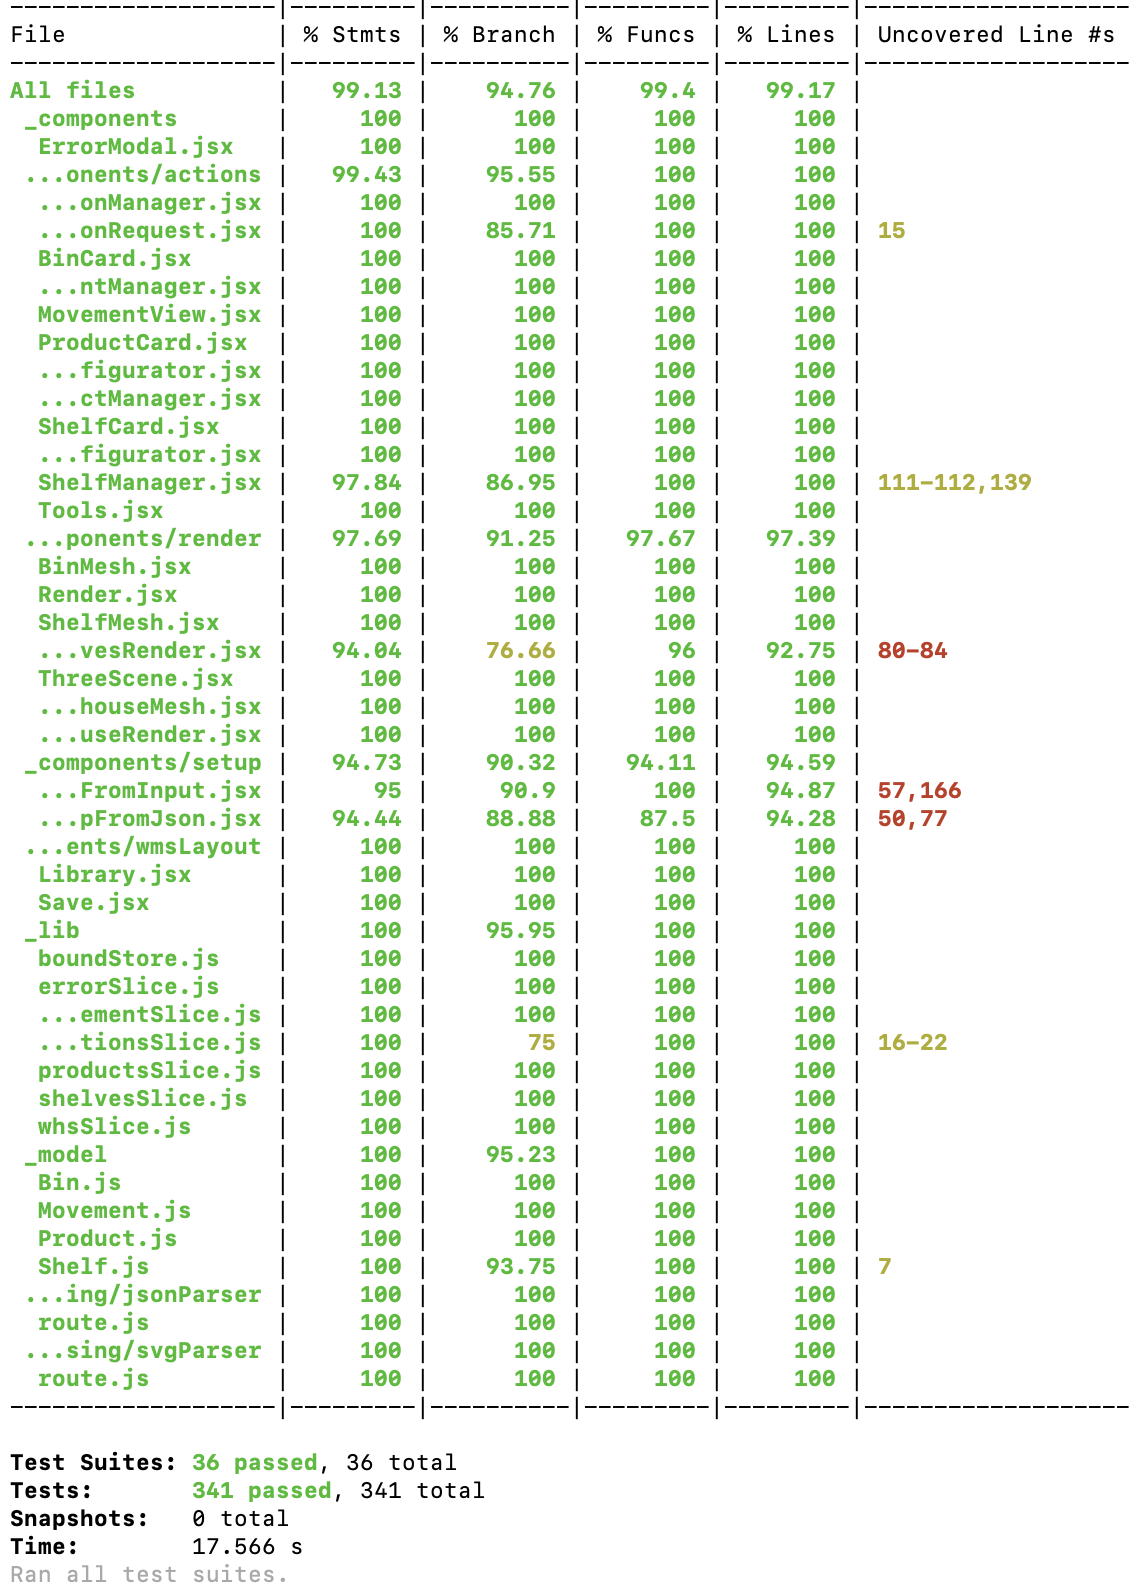
\includegraphics[width=0.8\textwidth]{images/MPC17-TP.png}
    \caption{MPC17-TP: Test Passed}
\end{figure}

\noindent \textbf{Considerazioni:} Come si evince dalla figura, tutti i test sono passati. Durante la fase di scrittura dei test quelli falliti hanno causato un aggiornamento istantaneo del codice e un successivo aggiornamento dello stato del test. 

\subsection{Qualità di prodotto}

\subsubsection{Qualità di prodotto - Customer Needs}

\paragraph{MPD1-ROB: Copertura dei requisiti obbligatori,  MPD2-RDE: Copertura dei requisiti desiderabili}
\begin{figure}[H] 
    \centering
    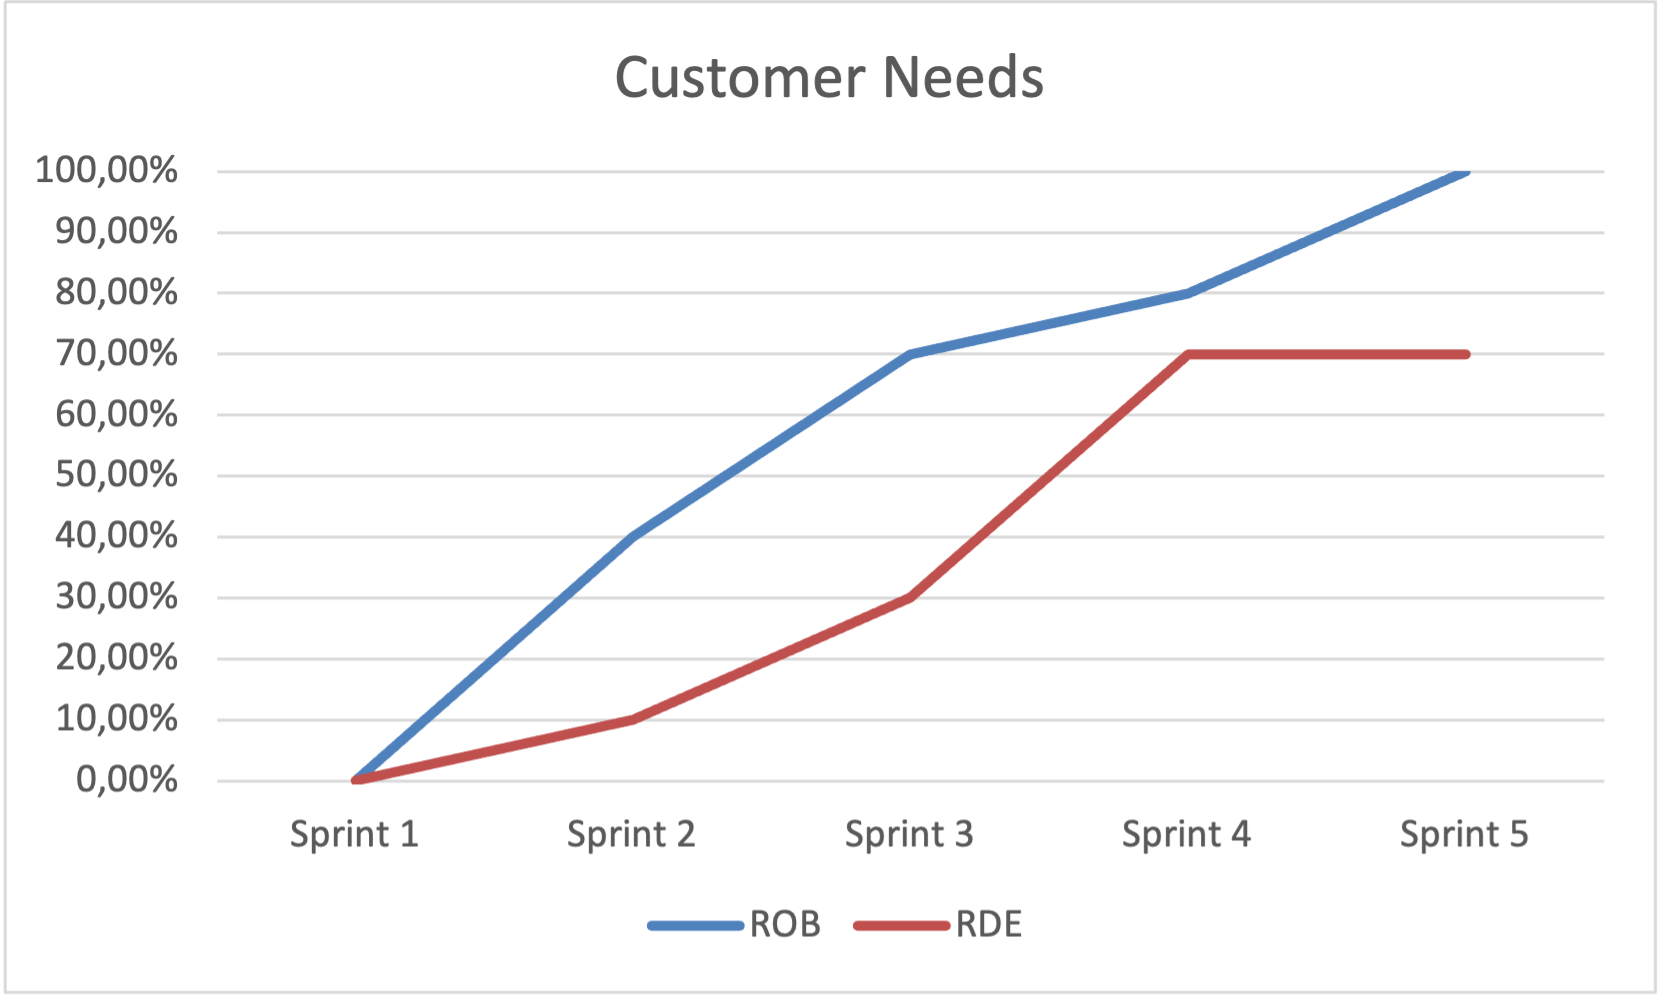
\includegraphics[width=0.8\textwidth]{images/Customer Needs.png}
    \caption{Customer Needs}
\end{figure}

\noindent \textbf{Considerazioni:} L'aumento di copertura di requisiti, sia desiderabili che obbligatori, è sempre stato costante e crescente. Non sono dunque servite azioni correttive.

Come si può notare in figura, le metriche MPD1-ROB e MPD2-RDE sono soddisfatte. Nello specifico, si raggiunge l'ottimalità per la metrica MPD1-ROB, mentre si rientra nei valori accettabili per la metrica MPD2-RDE.

\subsubsection{Qualità di prodotto - Efficienza}

\paragraph{MPD3-ART: Average Response Time}
L'unica funzione soggetta a visibile latenza è il caricamento del magazzino da file. Il tempo impiegato è tuttavia sempre inferiore a 2 secondi, pertanto la metrica MPD3-ART è soddisfatta.

\subsubsection{Qualità di prodotto - Usabilità}

\paragraph{MPD4-PC: Profondità Click}
Il numero di click che l'utente deve fare per poter raggiungere una determinata funzione non è mai superiore a 3, dunque la metrica MPD4-PC è soddisfatta.

\paragraph{MPD5-CFO: Comprensibilità funzionalità offerte}
Il prodotto finale è stato sottoposto ad un'analisi da parte dei componenti del gruppo non coinvolti direttamente nella programmazione, con risultati che sembrano dimostrare la facilità di comprensione delle funzionalità proposte. In particolare è stato assegnato un valore di 95\% alla metrica CFO.


\newpage
\subsubsection{Qualità di prodotto - Portabilità su altre piattaforme}
\paragraph{MPD6-PPT: Portabilità su piattaforme}
La metrica risulta essere soddisfatta dato il corretto funzionamento dell'applicativo nei browser richiesti. Si riporta di seguito la visualizzazione dell'applicativo nei vari browser, corredato dalla versione del browser in cui l'applicativo è stato testato.

\subparagraph{Google Chrome}
v124.0.6367.119 (Official Build) (arm64)
\begin{figure}[H] 
    \centering
    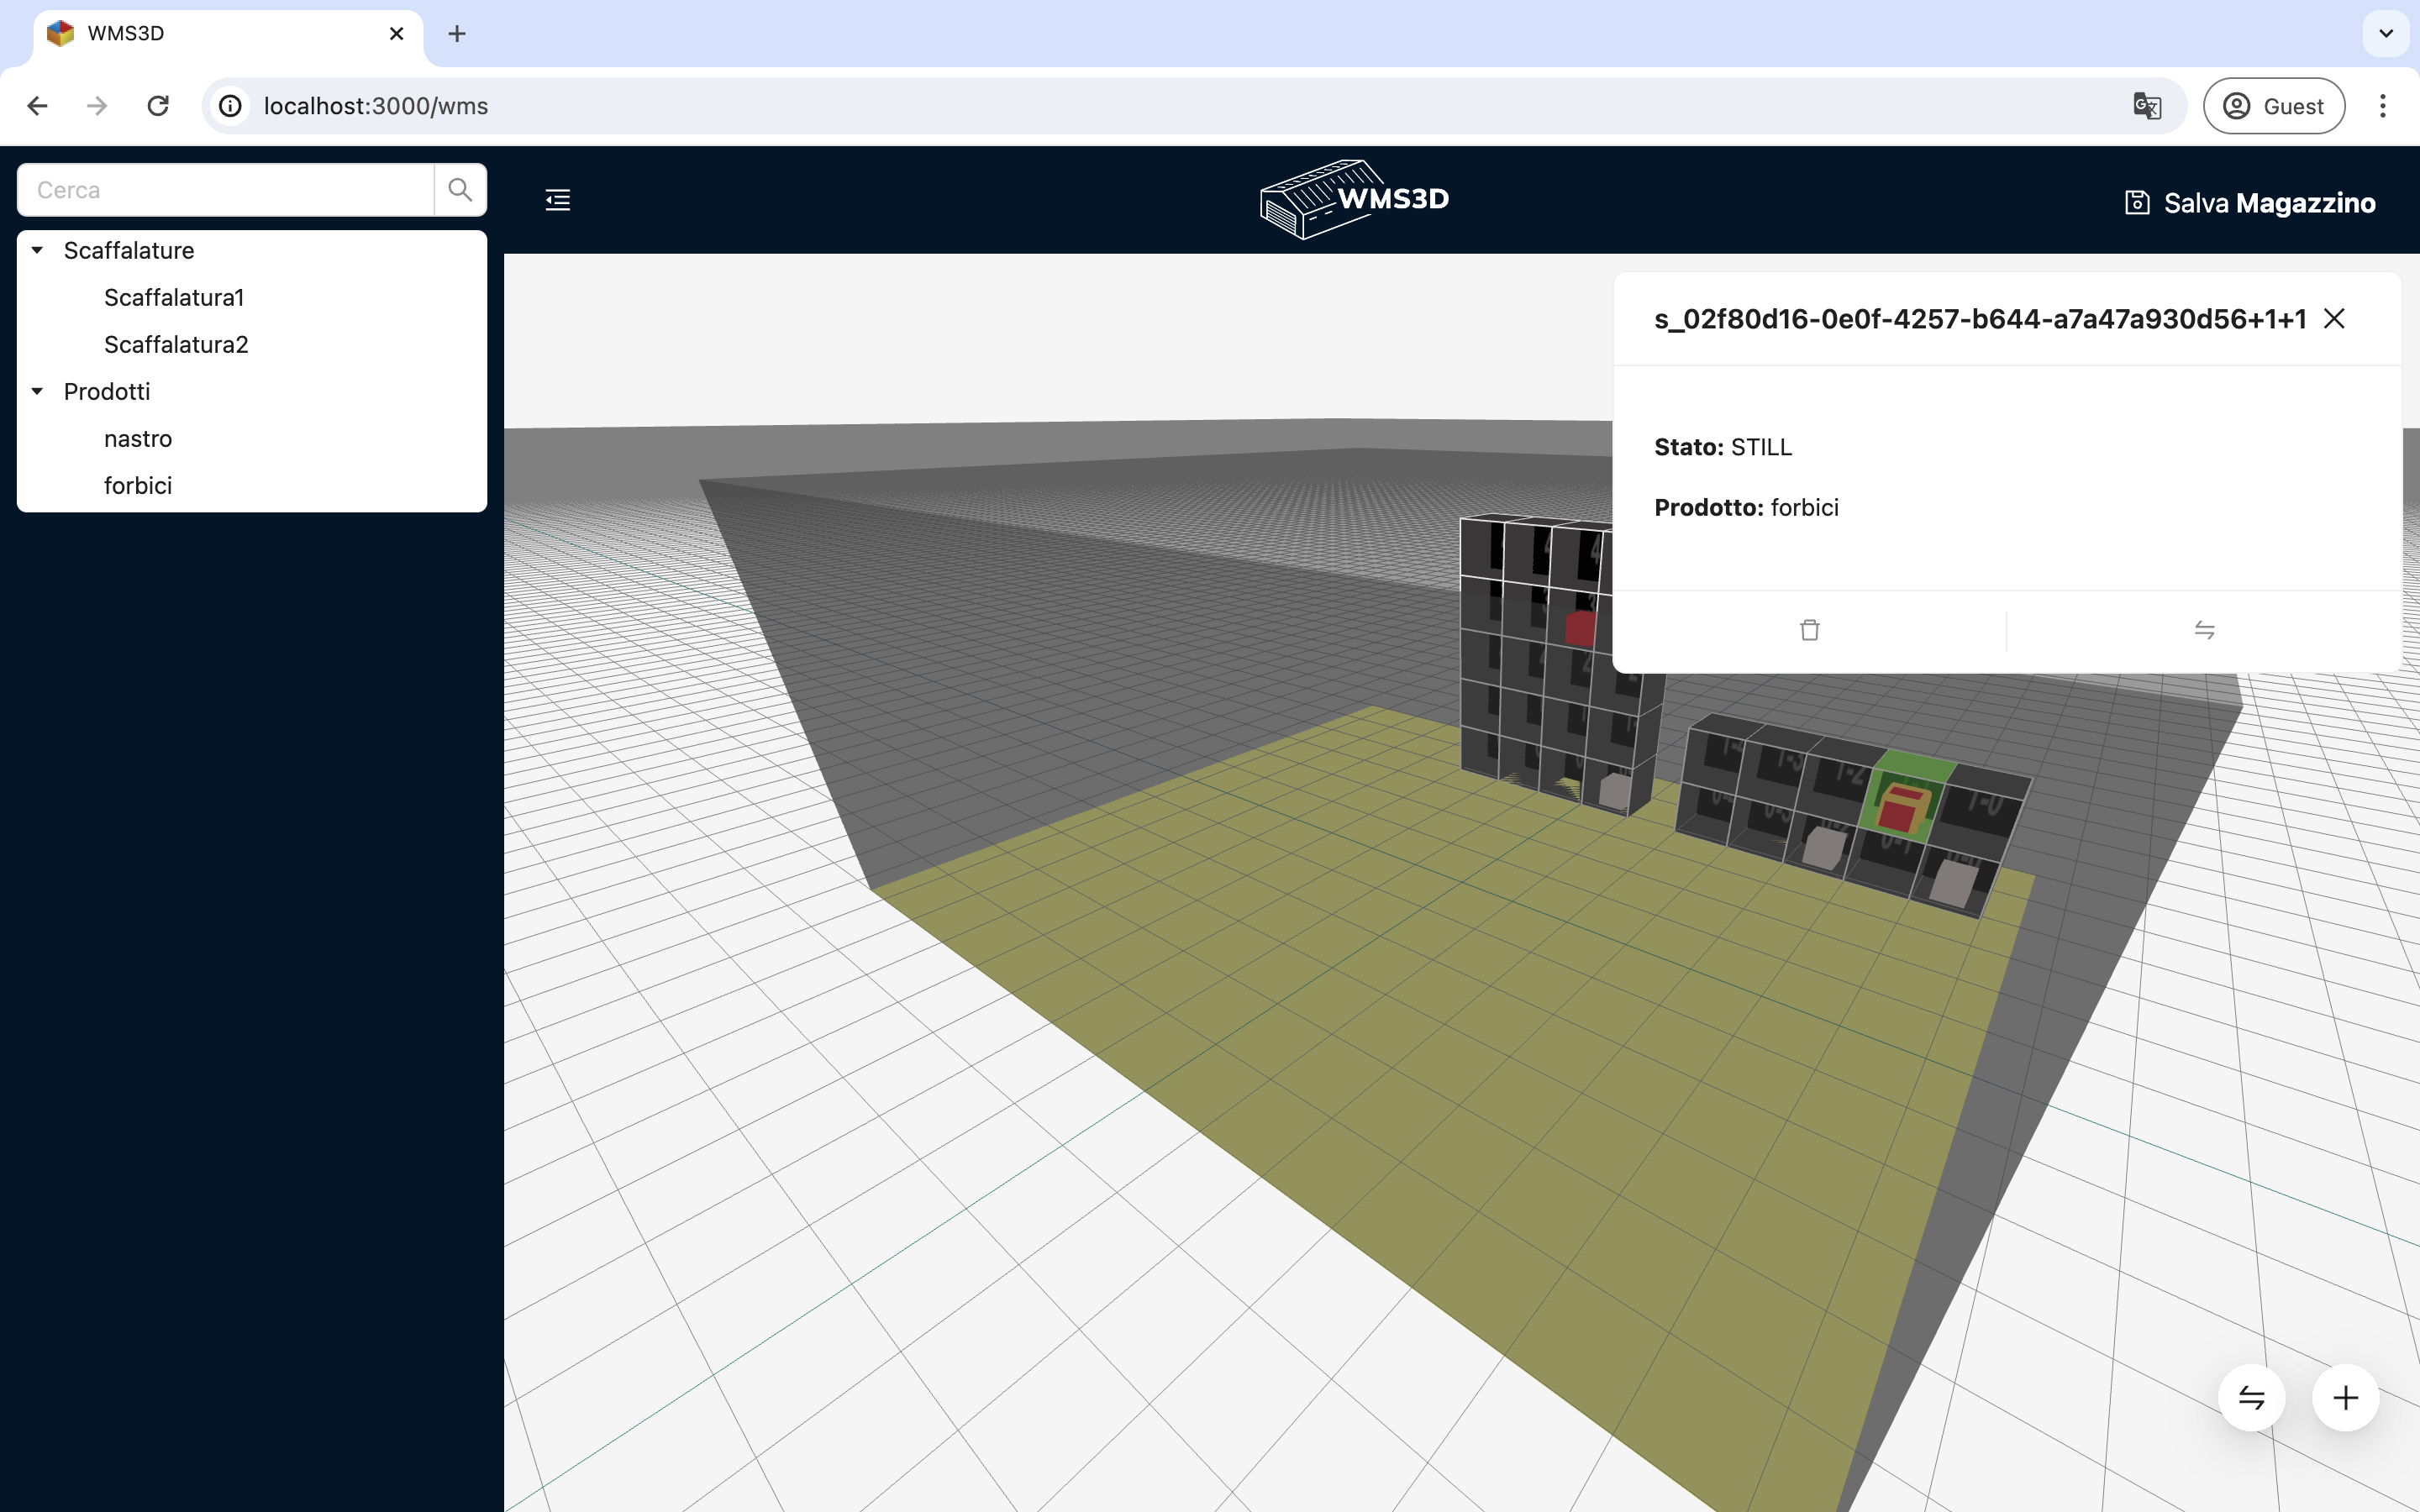
\includegraphics[width=0.8\textwidth]{images/chrome.png}
    \caption{Test su Google Chrome}
\end{figure}


\subparagraph{Safari}
v17.1.2 (19616.2.9.11.12)
\begin{figure}[H] 
    \centering
    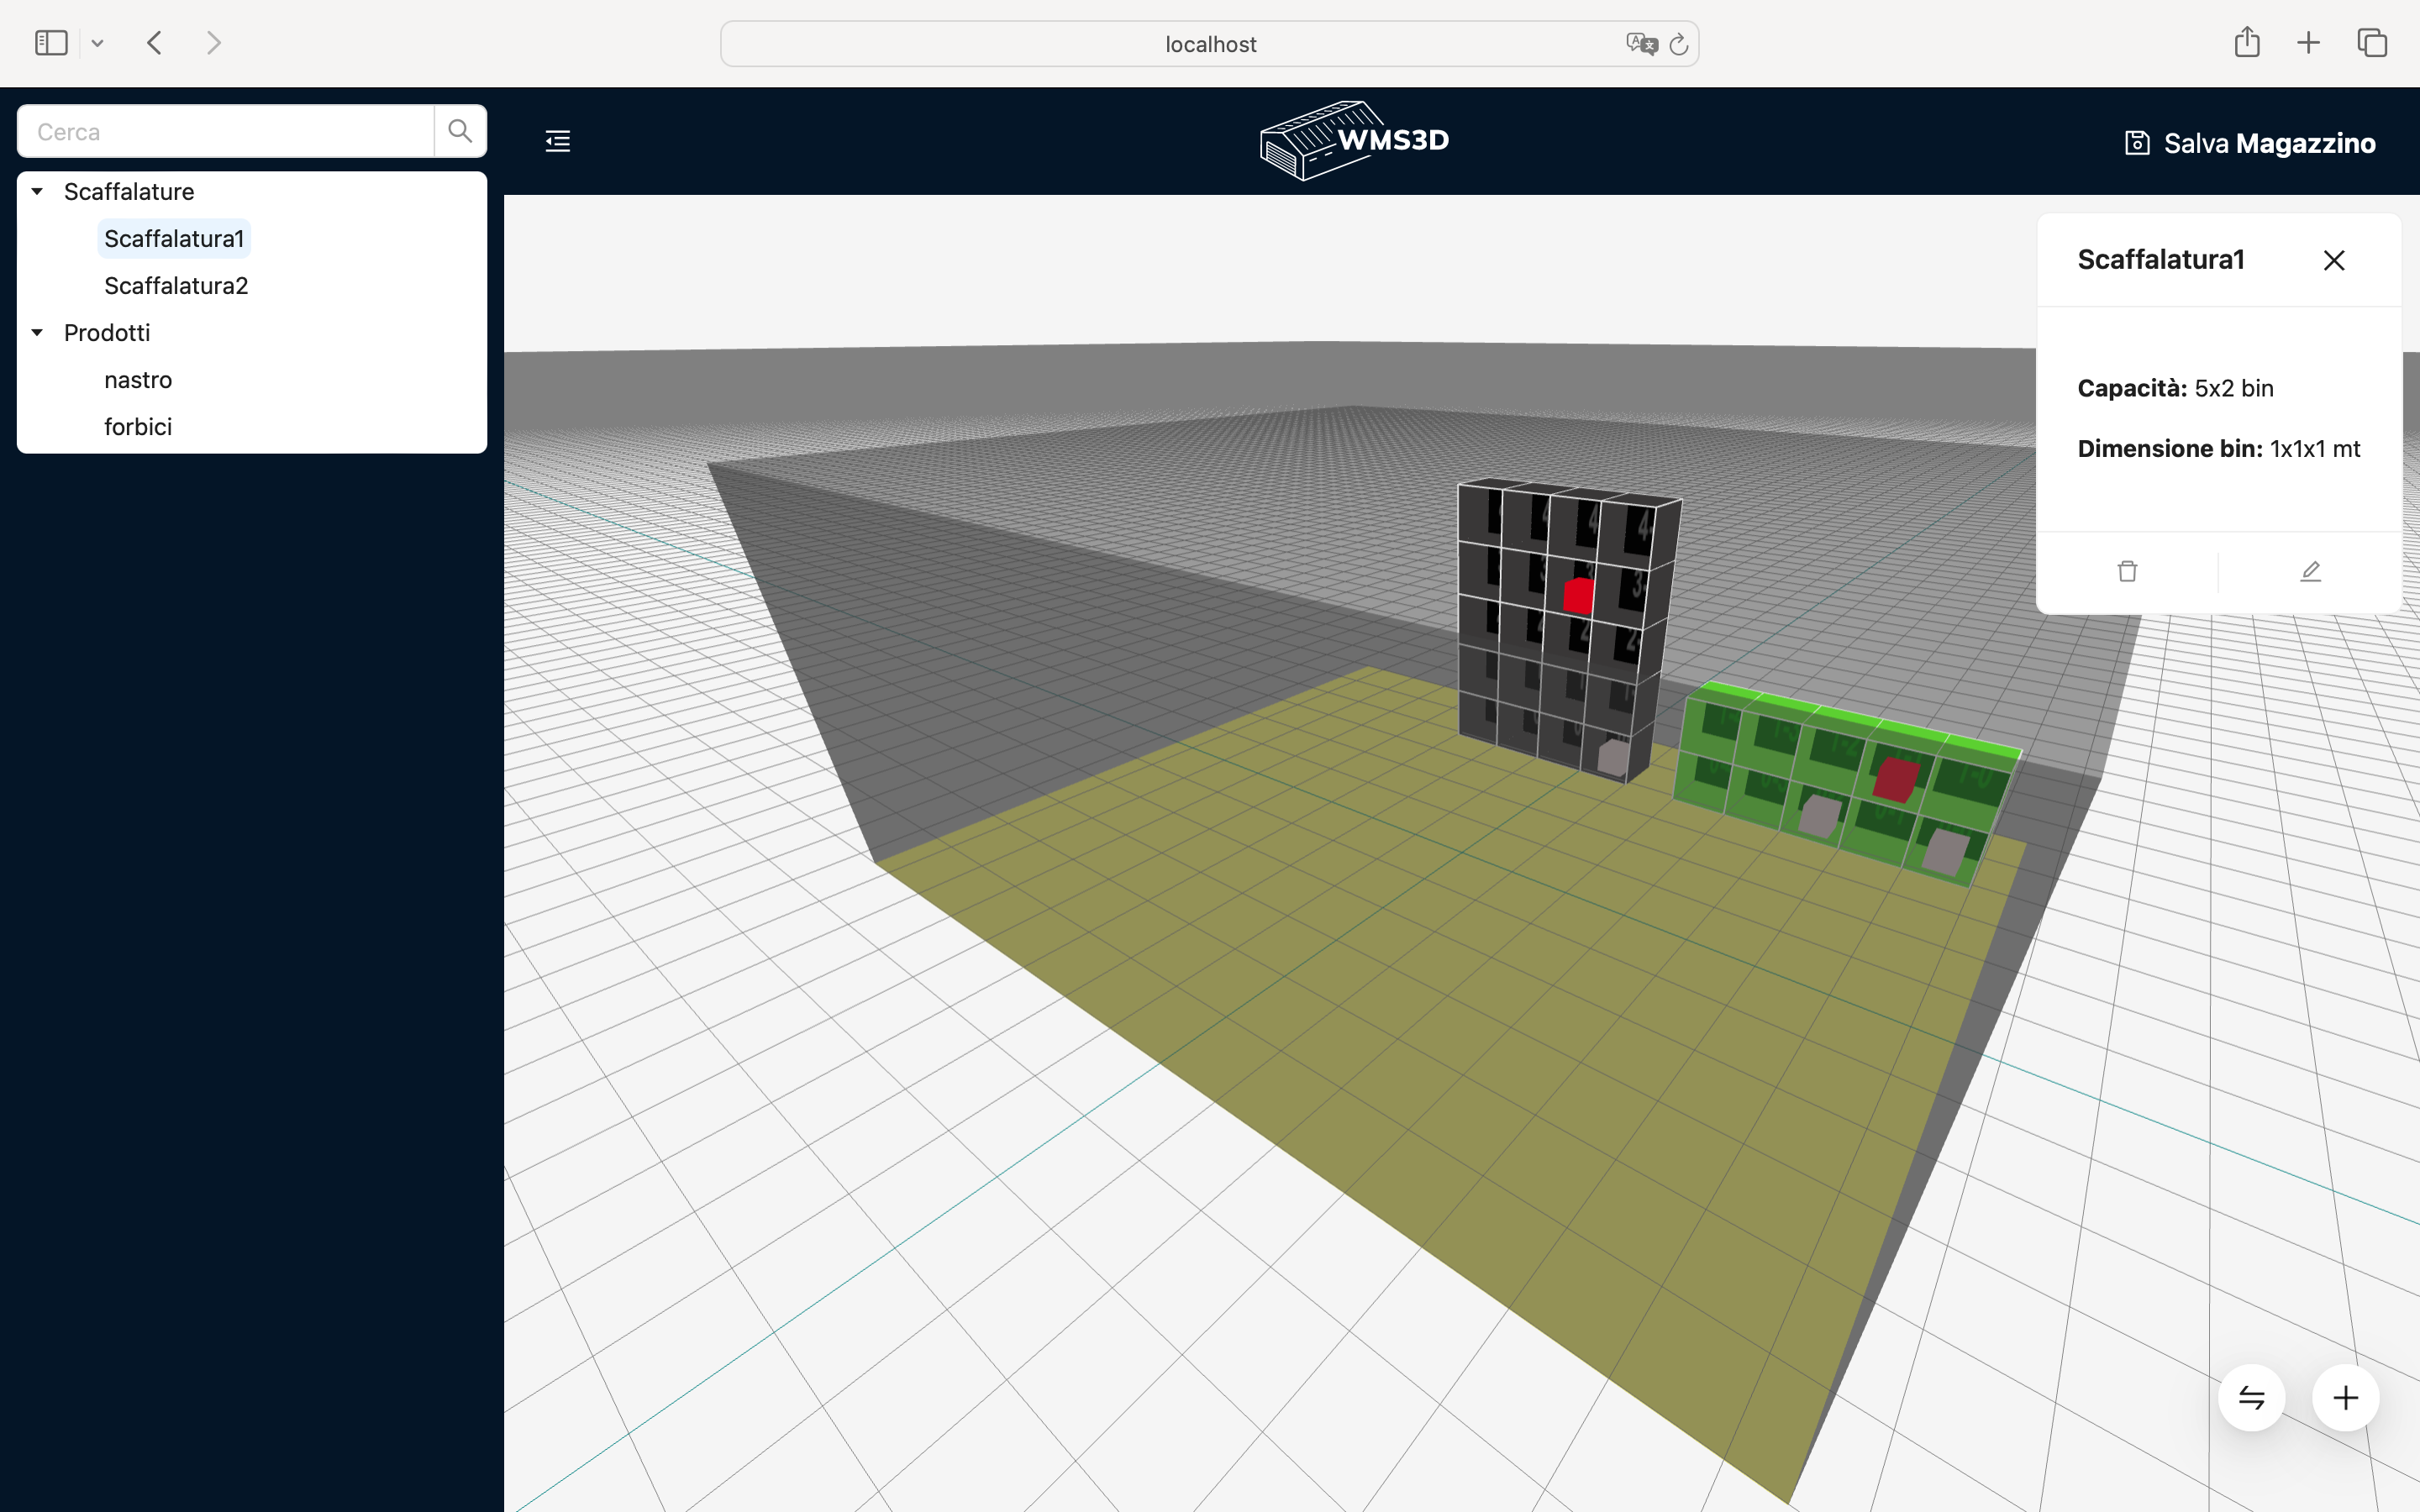
\includegraphics[width=0.8\textwidth]{images/safari.png}
    \caption{Test su Safari}
\end{figure}


\subparagraph{Firefox}
v115 (64-bit)
\begin{figure}[H] 
    \centering
    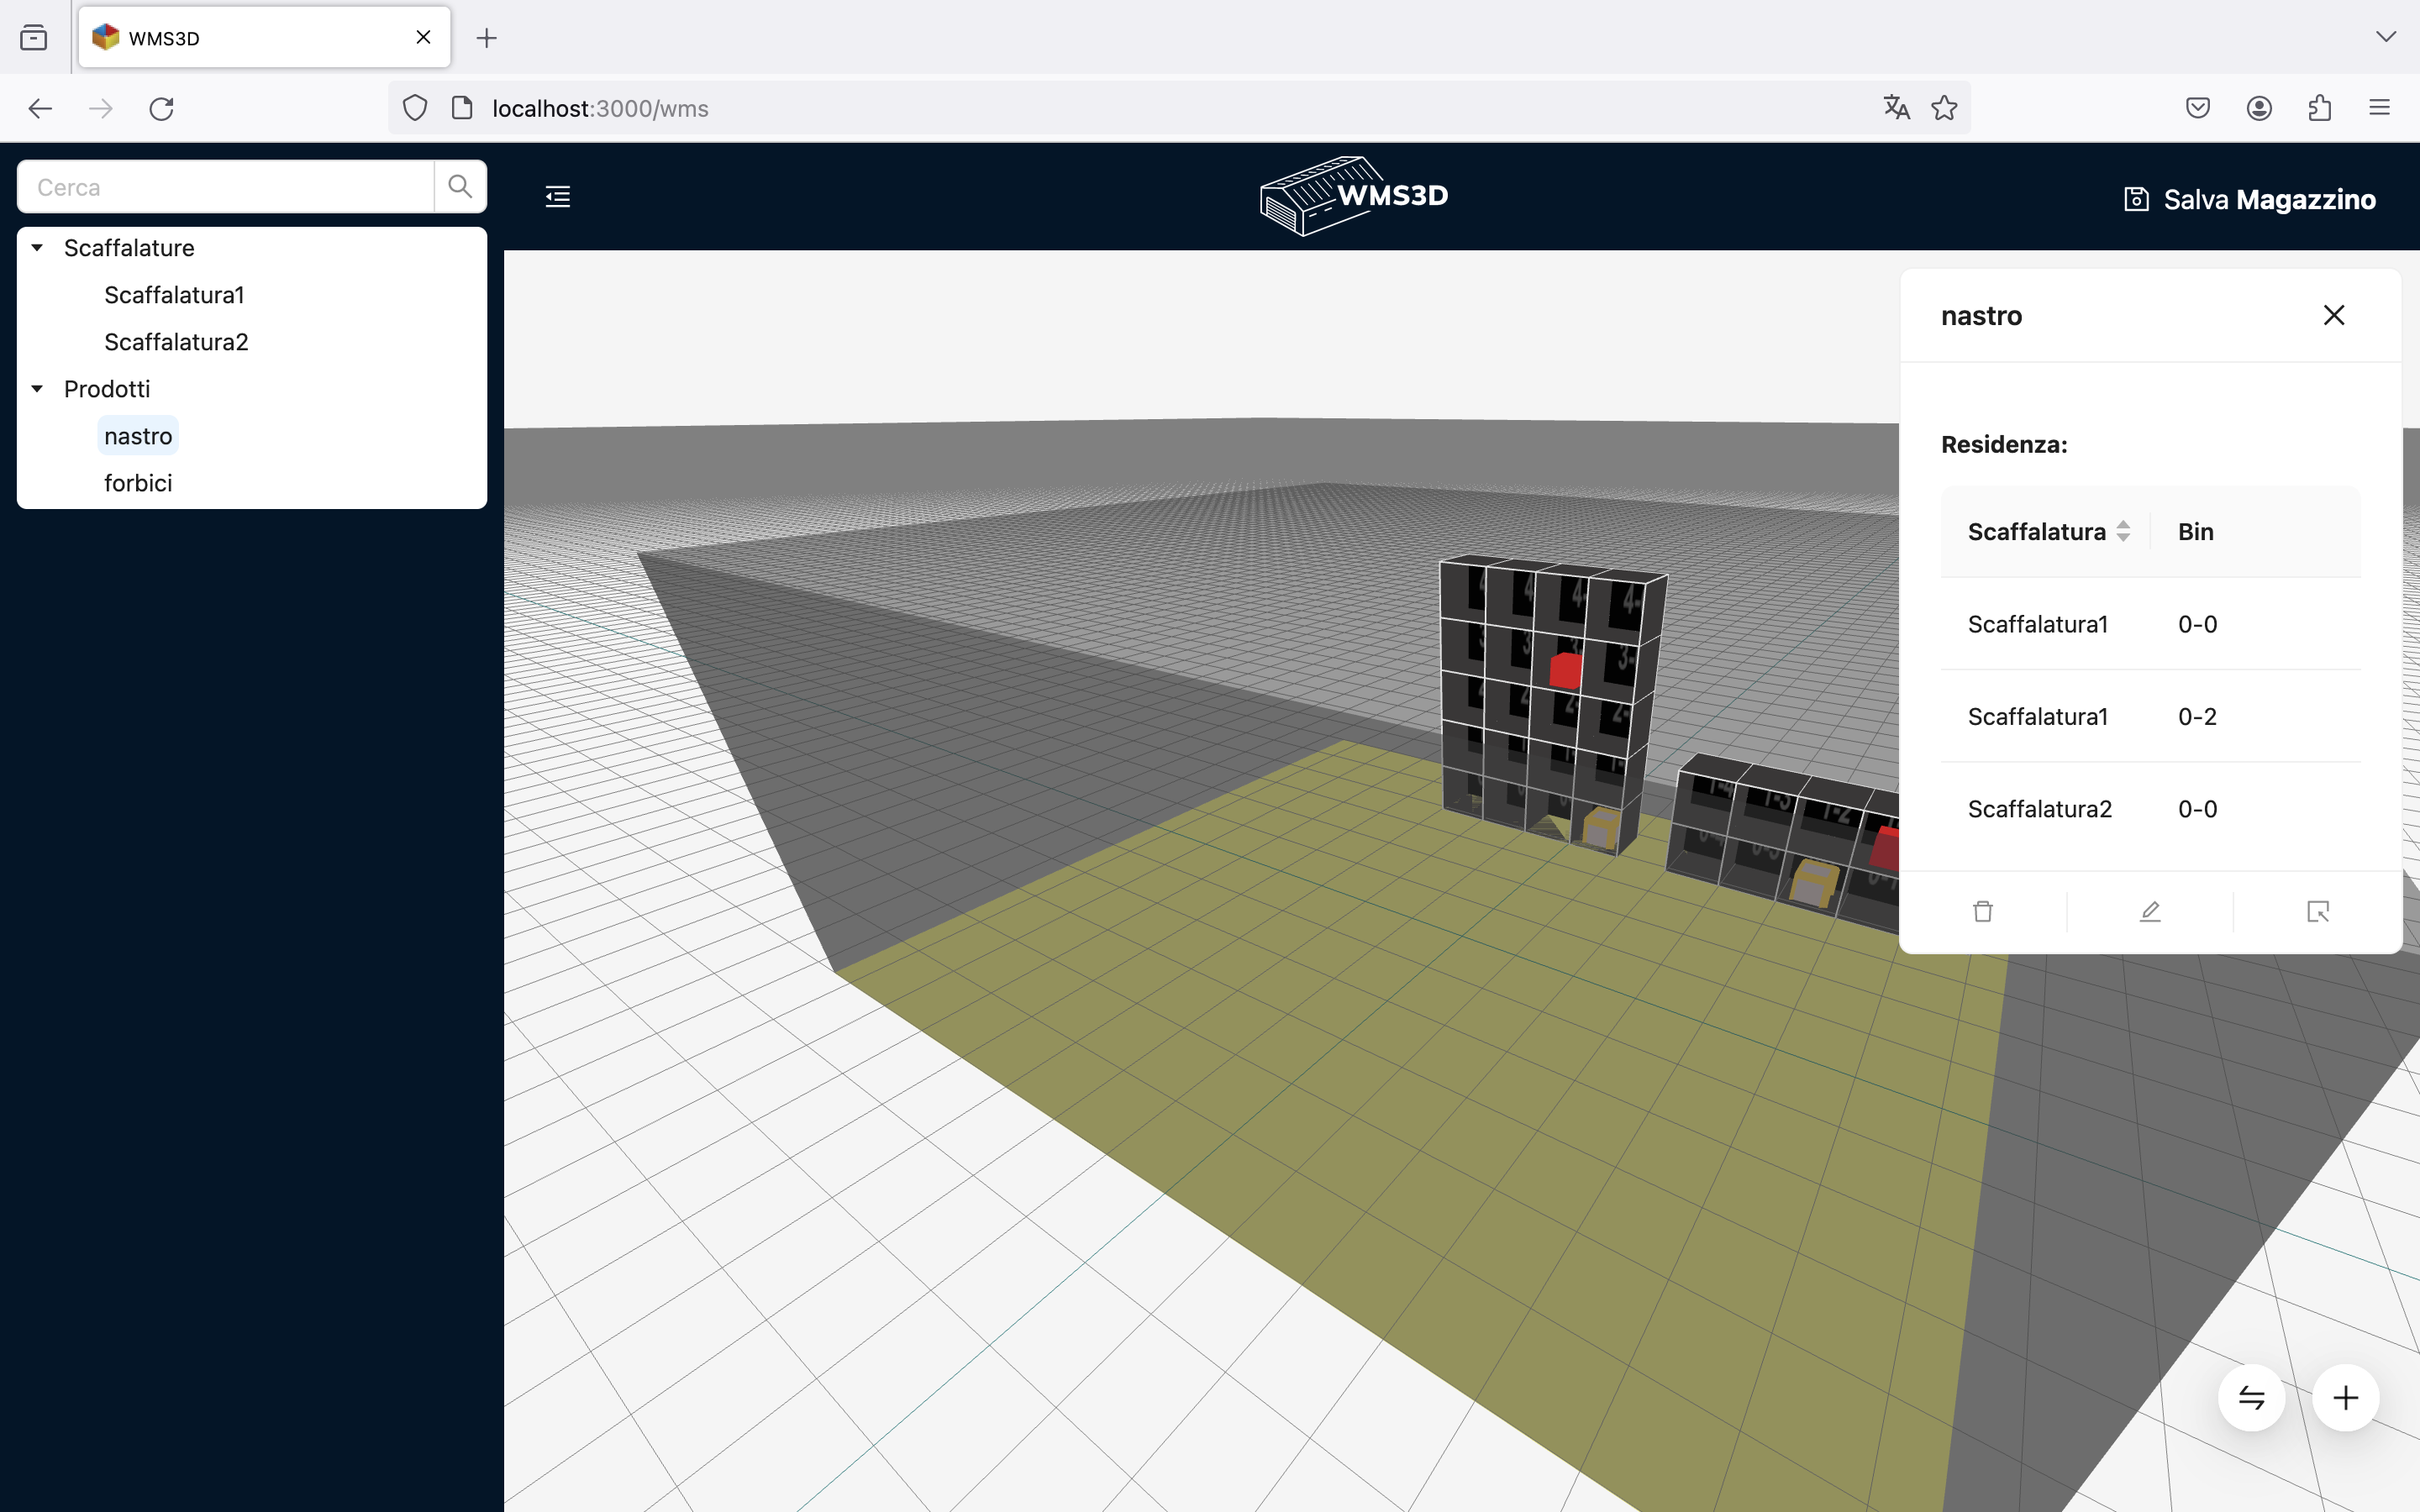
\includegraphics[width=0.8\textwidth]{images/firefox.png}
    \caption{Test su Firefox}
\end{figure}

\subparagraph{Opera}
v109.0.5097.68 (arm64)
\begin{figure}[H] 
    \centering
    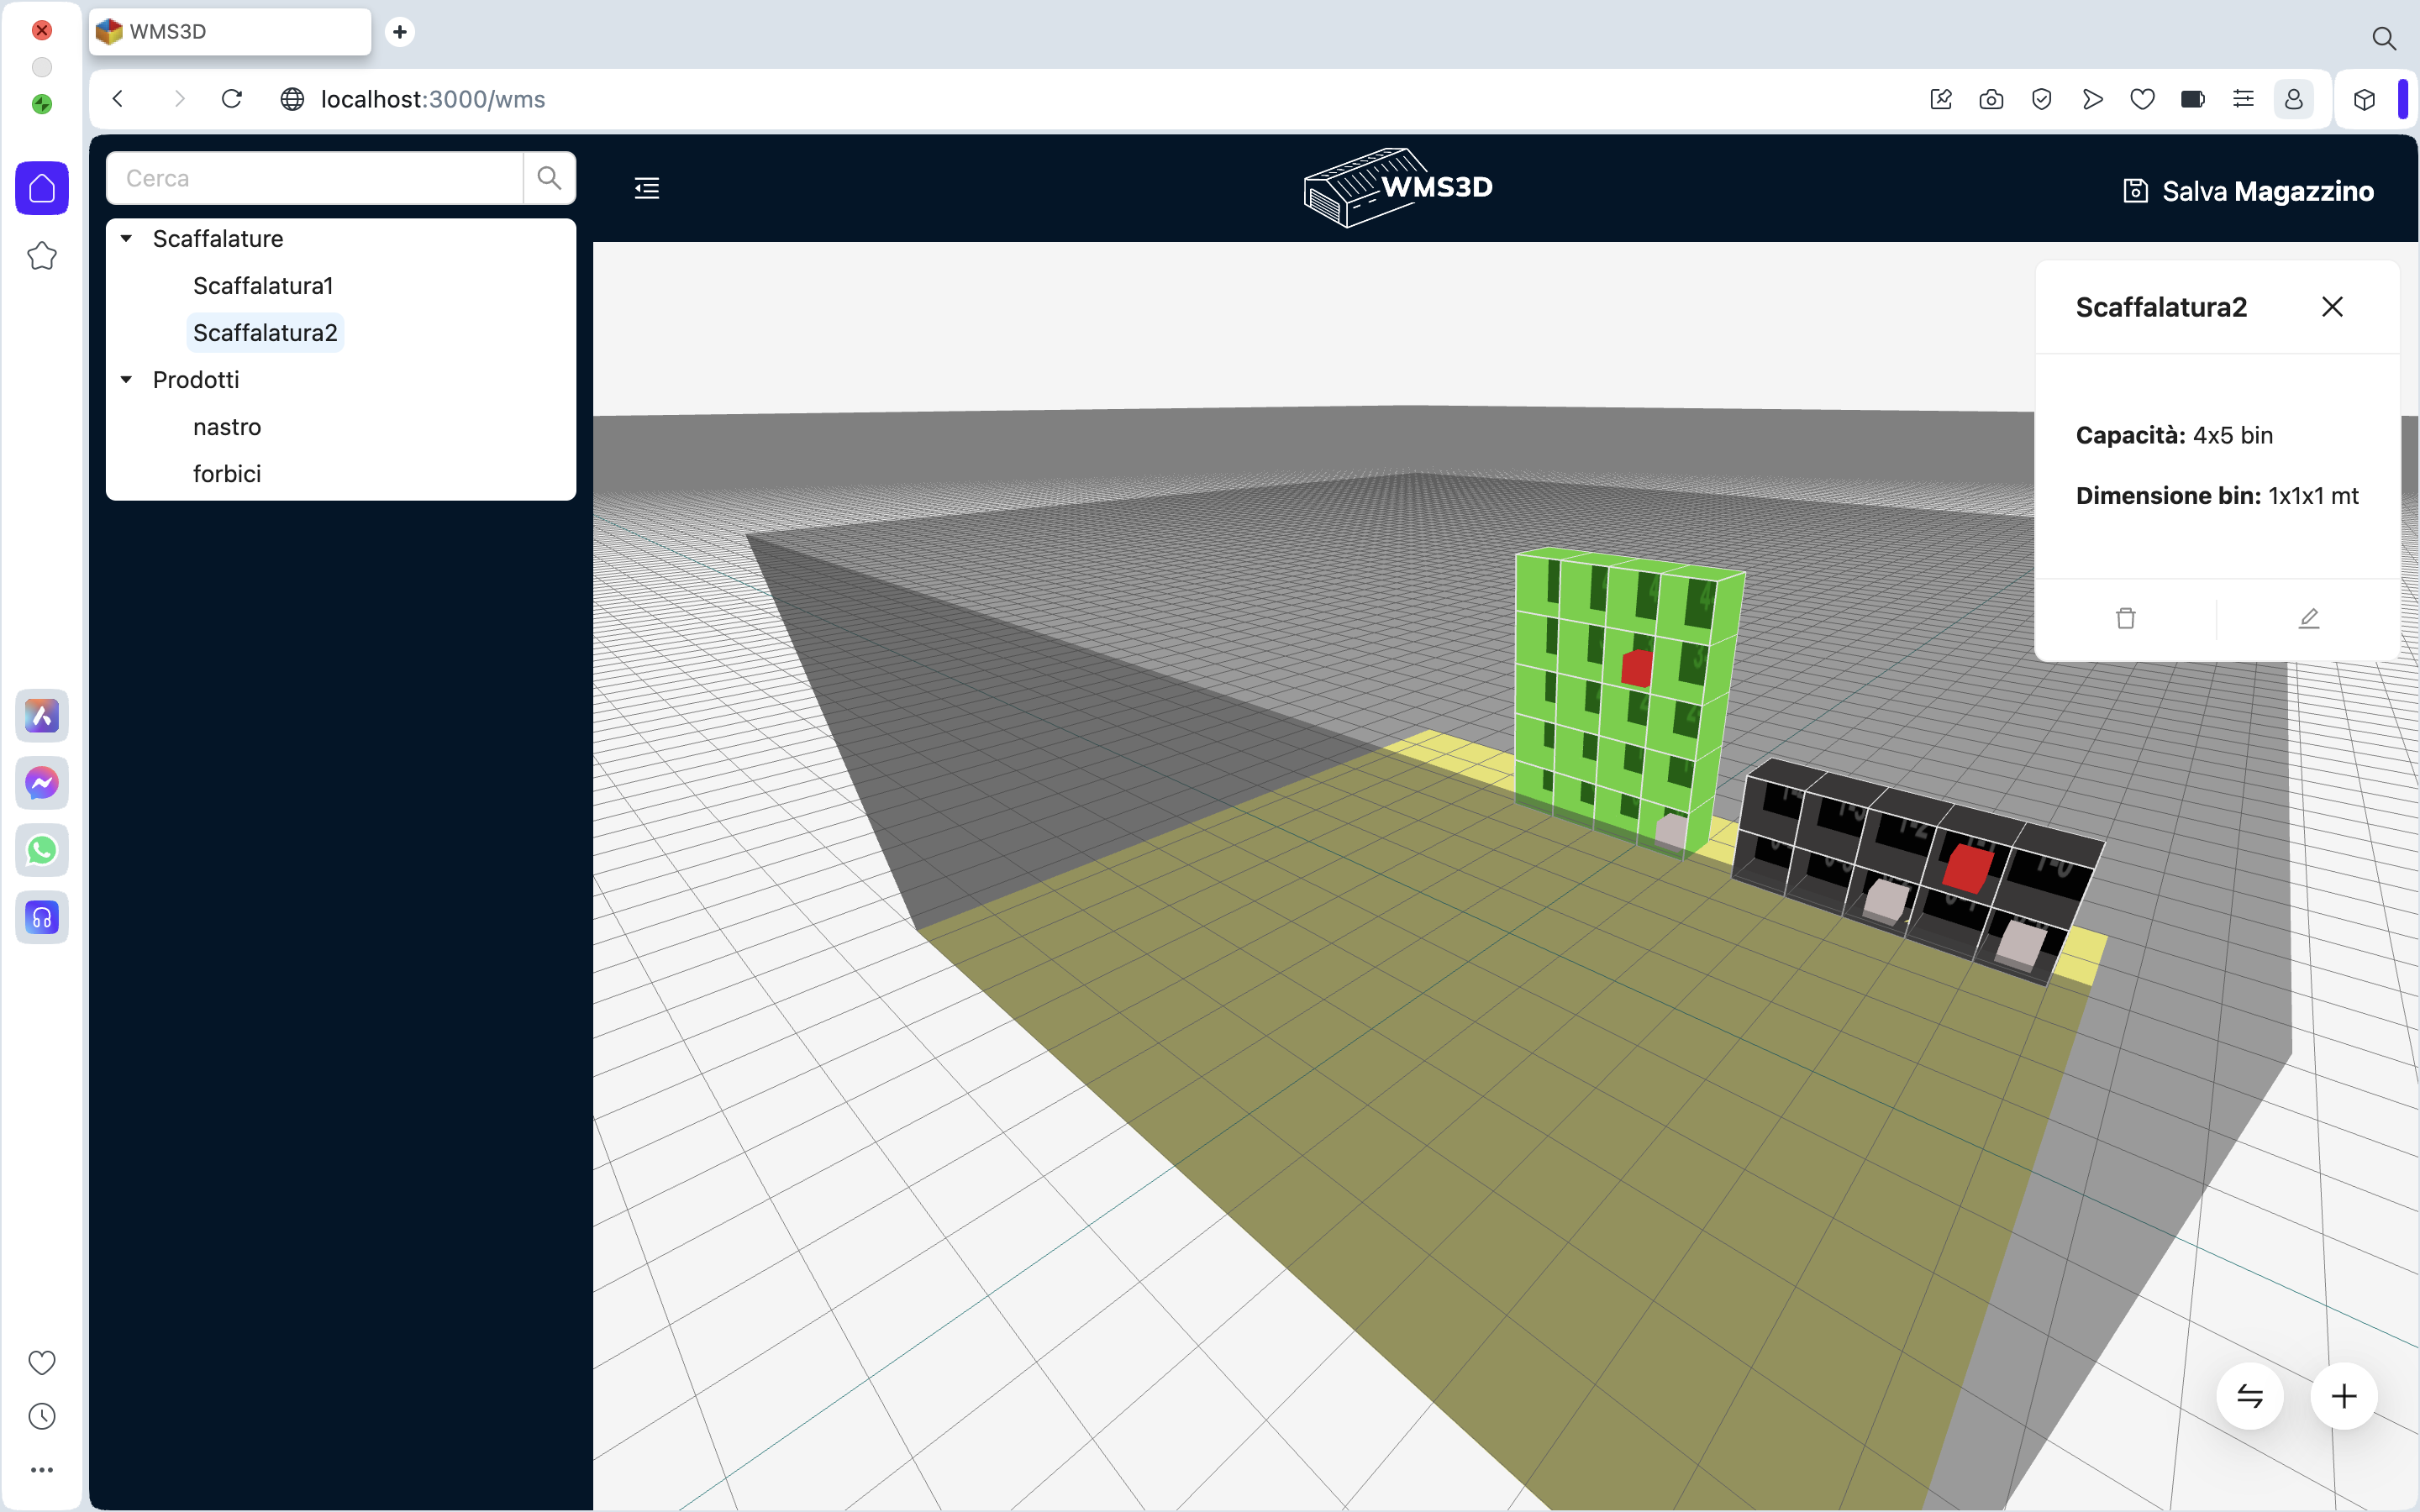
\includegraphics[width=0.8\textwidth]{images/opera.png}
    \caption{Test su Opera}
\end{figure}


\subparagraph{Microsoft Edge}
v124.0.2478.80 (Official build) (arm64)
\begin{figure}[H] 
    \centering
    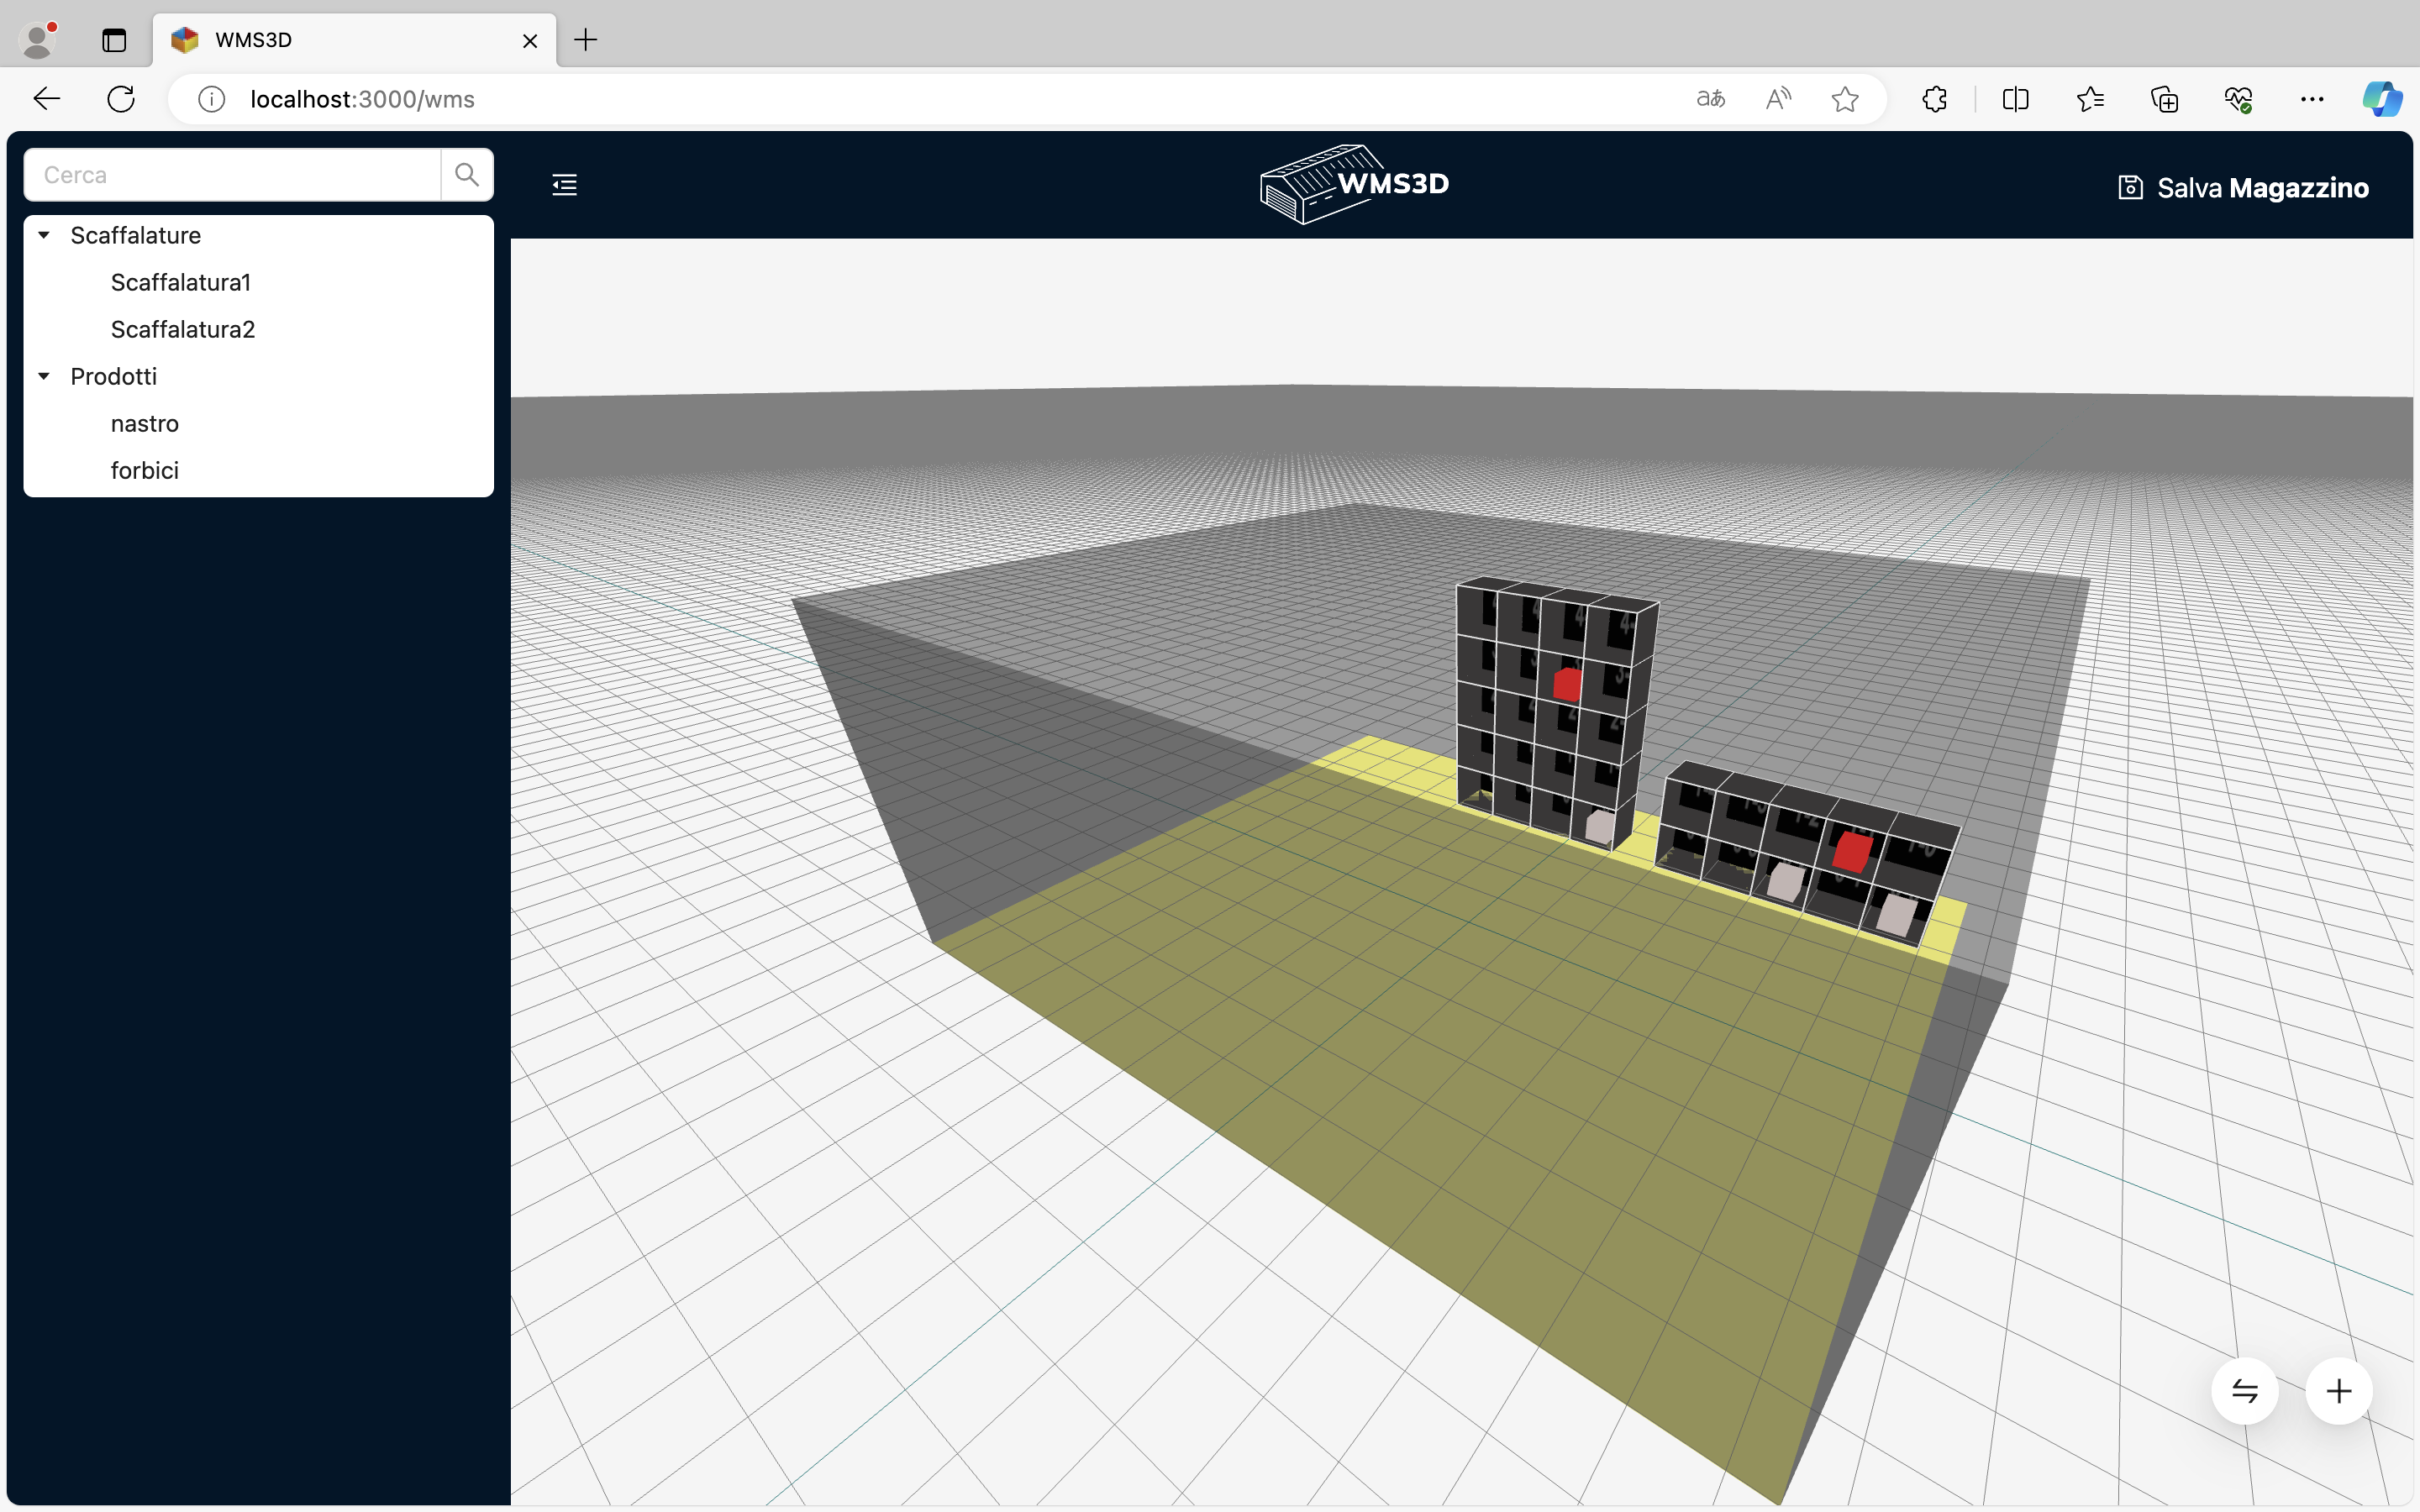
\includegraphics[width=0.8\textwidth]{images/microsoftedge.png}
    \caption{Test su Microsoft Edge}
\end{figure}


\newpage
\section{Riferimenti esterni} \label{sec:riferimenti_esterni}
Per ulteriori chiarimenti sugli argomenti discussi nel documento, si possono consultare i seguenti link esterni:
\begin{itemize}
    \item \textbf{Piano di Progetto v2.0.0}:\\
    \url{https://github.com/Avant-Garde-Software-Engineering/WMS3D/blob/main/Documentazione/PB/Esterna/piano_di_progetto_v2.0.0.pdf}
    \item \textbf{Specifica Tecnica v1.0.0}:\\
    \url{https://github.com/Avant-Garde-Software-Engineering/WMS3D/blob/main/Documentazione/PB/Esterna/specifica_tecnica_v1.0.0.pdf}
    \item \textbf{Norme di Progetto v4.0.0}:\\
    \url{https://github.com/Avant-Garde-Software-Engineering/WMS3D/blob/main/Documentazione/PB/Interna/norme_di_progetto_v4.0.0.pdf}
    \item \textbf{Analisi dei Requisiti v5.0.0}:\\
    \url{https://github.com/Avant-Garde-Software-Engineering/WMS3D/blob/main/Documentazione/PB/Esterna/analisi_dei_requisiti_v5.0.0.pdf}
    \item \textbf{Glossario v1.0.0}:\\
    \url{https://github.com/Avant-Garde-Software-Engineering/WMS3D/blob/main/Documentazione/PB/Esterna/glossario_v1.0.0.pdf}
    \item Capitolato \textbf{Warehouse Management 3D}:\\
    \url{https://www.math.unipd.it/~tullio/IS-1/2023/Progetto/C5.pdf}
    \item \textbf{Regolamento} del progetto didattico:\\
    \url{https://www.math.unipd.it/~tullio/IS-1/2023/Dispense/PD2.pdf}
    \item Link alla \textbf{documentazione del gruppo}:\\
    \url{https://avant-garde-software-engineering.github.io/documentazione.html} \textcolor{gray}{\textit{(ultimo accesso 13-05-24)}}
    \item Standard \textbf{ISO/IEC 12207}, versione 1995:\\
    \url{https://www.math.unipd.it/~tullio/IS-1/2009/Approfondimenti/ISO_12207-1995.pdf}
    \item Metriche di progetto, metodo \textbf{Earned Value}:\\
    \url{https://it.wikipedia.org/wiki/Metriche_di_progetto} \textcolor{gray}{\textit{(ultimo accesso 12-04-24)}}
\end{itemize}